%% =====================================================================
%% Journal manuscript for Biomedical Signal Processing and Control (Elsevier)
%% Review (preprint) format, elsarticle class. Compile on Overleaf with
%% pdfLaTeX + BibTeX (see README.md in this folder).
%%
%% All model-result numbers come from ../shared/results_macros.tex, which is
%% regenerated from the final model (python -m lungai.evaluation.render_docs).
%% Never type a model-result number by hand. Result-dependent interpretation
%% is marked with \pending{...}. The final model is fixed (run 2, v6.1,
%% chosen on the common validation set); as of 2026-11-04 no \pending items
%% remain: the seed-variability runs (runs 3-4, \RMS... macros) and the
%% preprocessing ablation (run 5, \RAbl... macros) are finished and written up.
%%
%% ---------------------------------------------------------------------
%% PLANNED EXTENSIONS: STATUS (updated 2026-11-03 evening)
%% ---------------------------------------------------------------------
%% DONE (results in the manuscript):
%%  - Source-identifiability probe: logistic regression on frozen 1024-d GAP
%%    features (ImageNet and trained backbone), overall and within class
%%    (lungai/evaluation/source_probe.py ->
%%    artifacts/data_quality/source_probe_v6_build_002.json; Sec. 4, 6).
%%  - Per-source analysis of the internal test split (Table tab:persource).
%%  - Run 1 vs run 2 on the common selection set with exact McNemar test
%%    (descriptive) and the shared-sources-only restriction.
%%
%% DONE 2026-11-04 (finished, in the manuscript):
%%  - Seeds 43 and 44 of the selected configuration (runs 3-4), reported with
%%    run 2 as mean +/- SD (3 runs only) -> Sec. "Seed variability".
%%  - No-filter preprocessing ablation, seed 42 (run 5), one seed -> Sec.
%%    "Preprocessing ablation". Only full chain vs no filters; no single-
%%    filter or canonical-size-first variants.
%%
%% NOT DONE (do not claim; do before submission or keep as limitations):
%%  1. A second backbone (e.g. ResNet-50, EfficientNet-B0) under the
%%     identical leakage-controlled protocol.
%%  2. Statistical comparison beyond McNemar on the common set: DeLong or
%%     paired bootstrap for ROC-AUC differences; seed-based comparison of
%%     runs (3 seeds of one configuration are not enough for this).
%%  3. A second external cohort with more than two classes (e.g. VinDr-CXR,
%%     PadChest, or a local hospital set with ethics approval).
%%  4. Quantitative evaluation of the CXR input gate on real non-radiograph
%%     images (threshold 0.703 checked with synthetic negatives only).
%%  5. Post-hoc calibration (temperature scaling fitted on validation) and a
%%     validated "inconclusive" threshold.
%%  6. Public code release (repository URL) and CLAIM / TRIPOD+AI
%%     checklists as supplementary material.
%%  Also not done: leave-one-source-out training or lung-masked inference
%%  (a causal test of the source shortcut); finer preprocessing ablation.
%% =====================================================================

\documentclass[preprint,12pt]{elsarticle}

\usepackage[T1]{fontenc}
\usepackage[utf8]{inputenc}
\usepackage{amsmath,amssymb}
\usepackage{graphicx}
\usepackage{booktabs}
\usepackage{xcolor}
\usepackage{url}
\usepackage[hidelinks]{hyperref}
\usepackage{lineno}

\newcommand{\pending}[1]{\textcolor{red}{[PENDING FINAL RESULTS: #1]}}
\newcommand{\confirm}[1]{\textcolor{blue}{[AUTHORS TO CONFIRM: #1]}}
% Use \protect\pending / \protect\confirm inside captions and other moving arguments.

% Generated by python -m lungai.evaluation.render_docs from artifacts/evaluation_reports/model_metrics.json.
% Source generated_at 2026-11-03T23:25:06+00:00. Do not edit by hand.
\providecommand{\xspace}{}
\newcommand{\RModelVersion}{v6.1}
\newcommand{\RDatasetBuild}{v6\_build\_002}
\newcommand{\RCheckpointShort}{7992b8da10ff}
\newcommand{\RSeed}{42}
\newcommand{\RNTrain}{10,957}
\newcommand{\RNVal}{2,348}
\newcommand{\RNTest}{2,350}
\newcommand{\RNExternal}{138}
\newcommand{\RSelectedEpoch}{16}
\newcommand{\REpochsTrained}{16}
\newcommand{\RValAcc}{76.9}
\newcommand{\RValMacroFOne}{78.5}
\newcommand{\RValMacroAUC}{0.953}
\newcommand{\RTestAcc}{77.4}
\newcommand{\RTestAccLo}{75.7}
\newcommand{\RTestAccHi}{79.0}
\newcommand{\RTestMacroFOne}{78.8}
\newcommand{\RTestWeightedFOne}{77.7}
\newcommand{\RTestMacroRecall}{78.1}
\newcommand{\RTestMacroPrecision}{79.9}
\newcommand{\RTestMacroAUC}{0.955}
\newcommand{\RTestMacroPRAUC}{0.849}
\newcommand{\RTestECE}{0.020}
\newcommand{\RExtSensK}{55}
\newcommand{\RExtSensN}{58}
\newcommand{\RExtSens}{94.8}
\newcommand{\RExtSensLo}{85.9}
\newcommand{\RExtSensHi}{98.2}
\newcommand{\RExtSpecK}{19}
\newcommand{\RExtSpecN}{80}
\newcommand{\RExtSpec}{23.8}
\newcommand{\RExtSpecLo}{15.8}
\newcommand{\RExtSpecHi}{34.1}
\newcommand{\RExtAUC}{0.809}
\newcommand{\RExtTBK}{0}
\newcommand{\RExtTBN}{58}
\newcommand{\RExtTB}{0.0}
\newcommand{\RExtCovidCalls}{3}
\newcommand{\RSupportCovid}{451}
\newcommand{\RPrecisionCovid}{96.6}
\newcommand{\RRecallCovid}{93.8}
\newcommand{\RSpecificityCovid}{99.2}
\newcommand{\RFOneCovid}{95.2}
\newcommand{\RAUCCovid}{0.994}
\newcommand{\RSupportNormal}{467}
\newcommand{\RPrecisionNormal}{75.5}
\newcommand{\RRecallNormal}{66.6}
\newcommand{\RSpecificityNormal}{94.6}
\newcommand{\RFOneNormal}{70.8}
\newcommand{\RAUCNormal}{0.937}
\newcommand{\RSupportEffusion}{444}
\newcommand{\RPrecisionEffusion}{70.1}
\newcommand{\RRecallEffusion}{82.0}
\newcommand{\RSpecificityEffusion}{91.9}
\newcommand{\RFOneEffusion}{75.6}
\newcommand{\RAUCEffusion}{0.954}
\newcommand{\RSupportPneumonia}{394}
\newcommand{\RPrecisionPneumonia}{91.3}
\newcommand{\RRecallPneumonia}{80.2}
\newcommand{\RSpecificityPneumonia}{98.5}
\newcommand{\RFOnePneumonia}{85.4}
\newcommand{\RAUCPneumonia}{0.949}
\newcommand{\RSupportNodule}{449}
\newcommand{\RPrecisionNodule}{57.0}
\newcommand{\RRecallNodule}{63.5}
\newcommand{\RSpecificityNodule}{88.7}
\newcommand{\RFOneNodule}{60.1}
\newcommand{\RAUCNodule}{0.904}
\newcommand{\RSupportTB}{145}
\newcommand{\RPrecisionTB}{88.9}
\newcommand{\RRecallTB}{82.8}
\newcommand{\RSpecificityTB}{99.3}
\newcommand{\RFOneTB}{85.7}
\newcommand{\RAUCTB}{0.994}
\newcommand{\RSrcNCohen}{111}
\newcommand{\RSrcAccCohen}{50.5}
\newcommand{\RSrcNCovidRad}{374}
\newcommand{\RSrcAccCovidRad}{99.5}
\newcommand{\RSrcNKermany}{398}
\newcommand{\RSrcAccKermany}{94.7}
\newcommand{\RSrcNNIH}{1124}
\newcommand{\RSrcAccNIH}{62.5}
\newcommand{\RSrcNShenzhen}{99}
\newcommand{\RSrcAccShenzhen}{80.8}
\newcommand{\RSrcNTBXk}{244}
\newcommand{\RSrcAccTBXk}{94.7}
\newcommand{\RCmpN}{2,018}
\newcommand{\RCmpSelected}{v6r2\_densenet121\_seed42}
\newcommand{\RCmpMcNemarB}{132}
\newcommand{\RCmpMcNemarC}{404}
\newcommand{\RCmpMcNemarP}{4.57e-33}
\newcommand{\RCmpRunOneN}{2,018}
\newcommand{\RCmpRunOneAcc}{63.5}
\newcommand{\RCmpRunOneMacroFOne}{59.4}
\newcommand{\RCmpRunOneMacroAUC}{0.880}
\newcommand{\RCmpRunOneSharedN}{1,392}
\newcommand{\RCmpRunOneSharedAcc}{67.6}
\newcommand{\RCmpRunOneSharedMacroFOne}{62.2}
\newcommand{\RCmpRunOneSharedMacroAUC}{0.929}
\newcommand{\RCmpRunTwoN}{2,018}
\newcommand{\RCmpRunTwoAcc}{77.0}
\newcommand{\RCmpRunTwoMacroFOne}{79.6}
\newcommand{\RCmpRunTwoMacroAUC}{0.957}
\newcommand{\RCmpRunTwoSharedN}{1,392}
\newcommand{\RCmpRunTwoSharedAcc}{67.8}
\newcommand{\RCmpRunTwoSharedMacroFOne}{68.5}
\newcommand{\RCmpRunTwoSharedMacroAUC}{0.929}
\newcommand{\RTestAccBootLo}{75.8}
\newcommand{\RTestAccBootHi}{79.1}
\newcommand{\RCxrGateNewThr}{0.703}
\newcommand{\RCxrGateValN}{2,348}
\newcommand{\RCxrGateValPassNew}{91.0}
\newcommand{\RCxrGateValPassOld}{38.7}
\newcommand{\RCxrGateBOneOldTestRej}{1,096}
\newcommand{\RCxrGateBOneOldTestN}{1,724}
\newcommand{\RCxrGateBOneOldTestRejPct}{63.6}
\newcommand{\RCxrGateBOneOldExtRej}{83}
\newcommand{\RCxrGateBOneOldExtN}{138}
\newcommand{\RCxrGateBOneOldExtRejPct}{60.1}
\newcommand{\RCxrGateBTwoNewTestRej}{218}
\newcommand{\RCxrGateBTwoNewTestN}{2,350}
\newcommand{\RCxrGateBTwoNewTestRejPct}{9.3}
\newcommand{\RCxrGateBTwoNewExtRej}{18}
\newcommand{\RCxrGateBTwoNewExtN}{138}
\newcommand{\RCxrGateBTwoNewExtRejPct}{13.0}
\newcommand{\RCxrGateBTwoOldTestRej}{1,494}
\newcommand{\RCxrGateBTwoOldTestN}{2,350}
\newcommand{\RCxrGateBTwoOldTestRejPct}{63.6}
\newcommand{\RCxrGateBTwoOldExtRej}{83}
\newcommand{\RCxrGateBTwoOldExtN}{138}
\newcommand{\RCxrGateBTwoOldExtRejPct}{60.1}
\newcommand{\RRunOneTestN}{1,724}
\newcommand{\RRunOneTestAcc}{65.7}
\newcommand{\RRunOneTestMacroFOne}{67.7}
\newcommand{\RRunOneTestMacroAUC}{0.921}
\newcommand{\RRunOneExtSensK}{45}
\newcommand{\RRunOneExtSpecK}{43}
\newcommand{\RRunOneExtAUC}{0.730}
\newcommand{\RRunOneExtTBK}{1}
\newcommand{\RRunOneExtCovidCalls}{71}
\newcommand{\RProbeNTrain}{1,952}
\newcommand{\RProbeNTest}{1,033}
\newcommand{\RProbeImgBalAcc}{93.8}
\newcommand{\RProbeImgChance}{16.7}
\newcommand{\RProbeImgNSources}{6}
\newcommand{\RProbeImgWithinCovid}{89.0}
\newcommand{\RProbeImgWithinCovidChance}{50.0}
\newcommand{\RProbeImgWithinCovidNSources}{2}
\newcommand{\RProbeImgWithinNormal}{97.2}
\newcommand{\RProbeImgWithinNormalChance}{20.0}
\newcommand{\RProbeImgWithinNormalNSources}{5}
\newcommand{\RProbeImgWithinPneumonia}{89.1}
\newcommand{\RProbeImgWithinPneumoniaChance}{33.3}
\newcommand{\RProbeImgWithinPneumoniaNSources}{3}
\newcommand{\RProbeImgWithinTB}{98.9}
\newcommand{\RProbeImgWithinTBChance}{33.3}
\newcommand{\RProbeImgWithinTBNSources}{3}
\newcommand{\RProbeMdlBalAcc}{93.8}
\newcommand{\RProbeMdlChance}{16.7}
\newcommand{\RProbeMdlNSources}{6}
\newcommand{\RProbeMdlWithinCovid}{89.2}
\newcommand{\RProbeMdlWithinCovidChance}{50.0}
\newcommand{\RProbeMdlWithinCovidNSources}{2}
\newcommand{\RProbeMdlWithinNormal}{97.4}
\newcommand{\RProbeMdlWithinNormalChance}{20.0}
\newcommand{\RProbeMdlWithinNormalNSources}{5}
\newcommand{\RProbeMdlWithinPneumonia}{88.4}
\newcommand{\RProbeMdlWithinPneumoniaChance}{33.3}
\newcommand{\RProbeMdlWithinPneumoniaNSources}{3}
\newcommand{\RProbeMdlWithinTB}{98.9}
\newcommand{\RProbeMdlWithinTBChance}{33.3}
\newcommand{\RProbeMdlWithinTBNSources}{3}
\newcommand{\RMSNRuns}{3}
\newcommand{\RMSSeeds}{42, 43, 44}
\newcommand{\RMSTestAccMean}{77.1}
\newcommand{\RMSTestAccMin}{76.9}
\newcommand{\RMSTestAccMax}{77.4}
\newcommand{\RMSTestAccSD}{0.3}
\newcommand{\RMSTestMacroFOneMean}{78.4}
\newcommand{\RMSTestMacroFOneMin}{77.9}
\newcommand{\RMSTestMacroFOneMax}{78.8}
\newcommand{\RMSTestMacroFOneSD}{0.4}
\newcommand{\RMSTestMacroAUCMean}{0.954}
\newcommand{\RMSTestMacroAUCMin}{0.953}
\newcommand{\RMSTestMacroAUCMax}{0.955}
\newcommand{\RMSTestMacroAUCSD}{0.001}
\newcommand{\RMSExtSensMean}{94.3}
\newcommand{\RMSExtSensMin}{93.1}
\newcommand{\RMSExtSensMax}{94.8}
\newcommand{\RMSExtSensSD}{1.0}
\newcommand{\RMSExtSpecMean}{27.1}
\newcommand{\RMSExtSpecMin}{23.8}
\newcommand{\RMSExtSpecMax}{31.2}
\newcommand{\RMSExtSpecSD}{3.8}
\newcommand{\RMSExtAUCMean}{0.788}
\newcommand{\RMSExtAUCMin}{0.762}
\newcommand{\RMSExtAUCMax}{0.809}
\newcommand{\RMSExtAUCSD}{0.024}
\newcommand{\RMSExtTBMean}{0.0}
\newcommand{\RMSExtTBMin}{0.0}
\newcommand{\RMSExtTBMax}{0.0}
\newcommand{\RMSExtTBSD}{0.0}
\newcommand{\RMSRunOneSeed}{42}
\newcommand{\RMSRunOneTestAcc}{77.4}
\newcommand{\RMSRunOneTestMacroFOne}{78.8}
\newcommand{\RMSRunOneTestMacroAUC}{0.955}
\newcommand{\RMSRunOneExtSens}{94.8}
\newcommand{\RMSRunOneExtSpec}{23.8}
\newcommand{\RMSRunOneExtTB}{0.0}
\newcommand{\RMSRunTwoSeed}{43}
\newcommand{\RMSRunTwoTestAcc}{77.1}
\newcommand{\RMSRunTwoTestMacroFOne}{78.5}
\newcommand{\RMSRunTwoTestMacroAUC}{0.954}
\newcommand{\RMSRunTwoExtSens}{93.1}
\newcommand{\RMSRunTwoExtSpec}{31.2}
\newcommand{\RMSRunTwoExtTB}{0.0}
\newcommand{\RMSRunThreeSeed}{44}
\newcommand{\RMSRunThreeTestAcc}{76.9}
\newcommand{\RMSRunThreeTestMacroFOne}{77.9}
\newcommand{\RMSRunThreeTestMacroAUC}{0.953}
\newcommand{\RMSRunThreeExtSens}{94.8}
\newcommand{\RMSRunThreeExtSpec}{26.2}
\newcommand{\RMSRunThreeExtTB}{0.0}
\newcommand{\RAblTestAcc}{74.1}
\newcommand{\RAblTestMacroFOne}{75.8}
\newcommand{\RAblTestMacroAUC}{0.949}
\newcommand{\RAblExtSpec}{23.8}
\newcommand{\RAblExtSens}{93.1}
\newcommand{\RAblExtTB}{8.6}
\newcommand{\RVFiveAcc}{82.9}
\newcommand{\RVFiveN}{1,570}
\newcommand{\RVFiveExtSpecK}{0}
\newcommand{\RVFiveExtSpecN}{80}
\newcommand{\RSpecSecPerImage}{0.113}
\newcommand{\RSpecTimingImages}{200}
\newcommand{\RSpecProjHoursMain}{1.6}
\newcommand{\RSpecProjHoursServed}{0.7}
\newcommand{\RSpecProjHoursNofilter}{0.7}
\newcommand{\RSpecProjHoursFeat}{1.0}
\newcommand{\RSpecMainValN}{1,019}
\newcommand{\RSpecMainValNTrain}{1,952}
\newcommand{\RSpecMainValChanceD}{0.45}
\newcommand{\RSpecMainValNWithinSources}{5}
\newcommand{\RSpecMainValFullSrcBA}{93.3}
\newcommand{\RSpecMainValFullSrcBALo}{91.5}
\newcommand{\RSpecMainValFullSrcBAHi}{95.0}
\newcommand{\RSpecMainValFullFWs}{71.3}
\newcommand{\RSpecMainValFullFWsLo}{68.2}
\newcommand{\RSpecMainValFullFWsHi}{74.4}
\newcommand{\RSpecMainValFullFAll}{64.6}
\newcommand{\RSpecMainValFullFAllLo}{61.6}
\newcommand{\RSpecMainValFullFAllHi}{67.7}
\newcommand{\RSpecMainValFullNormBA}{97.4}
\newcommand{\RSpecMainValFullNormBALo}{95.4}
\newcommand{\RSpecMainValFullNormBAHi}{99.0}
\newcommand{\RSpecMainValFullSStar}{0.920}
\newcommand{\RSpecMainValFullSStarLo}{0.898}
\newcommand{\RSpecMainValFullSStarHi}{0.940}
\newcommand{\RSpecMainValFullDStar}{0.479}
\newcommand{\RSpecMainValFullDStarLo}{0.421}
\newcommand{\RSpecMainValFullDStarHi}{0.535}
\newcommand{\RSpecMainValFullSDS}{0.441}
\newcommand{\RSpecMainValFullSDSLo}{0.379}
\newcommand{\RSpecMainValFullSDSHi}{0.505}
\newcommand{\RSpecMainValPassASrcBA}{68.6}
\newcommand{\RSpecMainValPassASrcBALo}{65.6}
\newcommand{\RSpecMainValPassASrcBAHi}{71.4}
\newcommand{\RSpecMainValPassAFWs}{59.5}
\newcommand{\RSpecMainValPassAFWsLo}{55.9}
\newcommand{\RSpecMainValPassAFWsHi}{62.6}
\newcommand{\RSpecMainValPassAFAll}{44.8}
\newcommand{\RSpecMainValPassAFAllLo}{41.6}
\newcommand{\RSpecMainValPassAFAllHi}{48.0}
\newcommand{\RSpecMainValPassANormBA}{82.5}
\newcommand{\RSpecMainValPassANormBALo}{78.6}
\newcommand{\RSpecMainValPassANormBAHi}{86.2}
\newcommand{\RSpecMainValPassASStar}{0.623}
\newcommand{\RSpecMainValPassASStarLo}{0.588}
\newcommand{\RSpecMainValPassASStarHi}{0.657}
\newcommand{\RSpecMainValPassADStar}{0.264}
\newcommand{\RSpecMainValPassADStarLo}{0.197}
\newcommand{\RSpecMainValPassADStarHi}{0.319}
\newcommand{\RSpecMainValPassASDS}{0.359}
\newcommand{\RSpecMainValPassASDSLo}{0.297}
\newcommand{\RSpecMainValPassASDSHi}{0.432}
\newcommand{\RSpecMainValPassBSrcBA}{63.1}
\newcommand{\RSpecMainValPassBSrcBALo}{60.2}
\newcommand{\RSpecMainValPassBSrcBAHi}{66.3}
\newcommand{\RSpecMainValPassBFWs}{56.6}
\newcommand{\RSpecMainValPassBFWsLo}{52.8}
\newcommand{\RSpecMainValPassBFWsHi}{59.8}
\newcommand{\RSpecMainValPassBFAll}{42.7}
\newcommand{\RSpecMainValPassBFAllLo}{39.4}
\newcommand{\RSpecMainValPassBFAllHi}{45.7}
\newcommand{\RSpecMainValPassBNormBA}{75.1}
\newcommand{\RSpecMainValPassBNormBALo}{70.3}
\newcommand{\RSpecMainValPassBNormBAHi}{79.8}
\newcommand{\RSpecMainValPassBSStar}{0.557}
\newcommand{\RSpecMainValPassBSStarLo}{0.522}
\newcommand{\RSpecMainValPassBSStarHi}{0.596}
\newcommand{\RSpecMainValPassBDStar}{0.211}
\newcommand{\RSpecMainValPassBDStarLo}{0.142}
\newcommand{\RSpecMainValPassBDStarHi}{0.269}
\newcommand{\RSpecMainValPassBSDS}{0.347}
\newcommand{\RSpecMainValPassBSDSLo}{0.282}
\newcommand{\RSpecMainValPassBSDSHi}{0.428}
\newcommand{\RSpecMainValPassCSrcBA}{70.5}
\newcommand{\RSpecMainValPassCSrcBALo}{67.7}
\newcommand{\RSpecMainValPassCSrcBAHi}{73.3}
\newcommand{\RSpecMainValPassCFWs}{56.9}
\newcommand{\RSpecMainValPassCFWsLo}{53.3}
\newcommand{\RSpecMainValPassCFWsHi}{59.9}
\newcommand{\RSpecMainValPassCFAll}{44.6}
\newcommand{\RSpecMainValPassCFAllLo}{41.3}
\newcommand{\RSpecMainValPassCFAllHi}{47.6}
\newcommand{\RSpecMainValPassCNormBA}{84.3}
\newcommand{\RSpecMainValPassCNormBALo}{80.5}
\newcommand{\RSpecMainValPassCNormBAHi}{87.8}
\newcommand{\RSpecMainValPassCSStar}{0.646}
\newcommand{\RSpecMainValPassCSStarLo}{0.612}
\newcommand{\RSpecMainValPassCSStarHi}{0.680}
\newcommand{\RSpecMainValPassCDStar}{0.216}
\newcommand{\RSpecMainValPassCDStarLo}{0.150}
\newcommand{\RSpecMainValPassCDStarHi}{0.270}
\newcommand{\RSpecMainValPassCSDS}{0.430}
\newcommand{\RSpecMainValPassCSDSLo}{0.367}
\newcommand{\RSpecMainValPassCSDSHi}{0.503}
\newcommand{\RSpecMainValPassDSrcBA}{79.1}
\newcommand{\RSpecMainValPassDSrcBALo}{76.5}
\newcommand{\RSpecMainValPassDSrcBAHi}{81.7}
\newcommand{\RSpecMainValPassDFWs}{64.8}
\newcommand{\RSpecMainValPassDFWsLo}{61.4}
\newcommand{\RSpecMainValPassDFWsHi}{68.0}
\newcommand{\RSpecMainValPassDFAll}{51.5}
\newcommand{\RSpecMainValPassDFAllLo}{48.5}
\newcommand{\RSpecMainValPassDFAllHi}{54.7}
\newcommand{\RSpecMainValPassDNormBA}{91.0}
\newcommand{\RSpecMainValPassDNormBALo}{87.8}
\newcommand{\RSpecMainValPassDNormBAHi}{94.2}
\newcommand{\RSpecMainValPassDSStar}{0.750}
\newcommand{\RSpecMainValPassDSStarLo}{0.718}
\newcommand{\RSpecMainValPassDSStarHi}{0.780}
\newcommand{\RSpecMainValPassDDStar}{0.360}
\newcommand{\RSpecMainValPassDDStarLo}{0.298}
\newcommand{\RSpecMainValPassDDStarHi}{0.418}
\newcommand{\RSpecMainValPassDSDS}{0.390}
\newcommand{\RSpecMainValPassDSDSLo}{0.330}
\newcommand{\RSpecMainValPassDSDSHi}{0.455}
\newcommand{\RSpecMainValPassESrcBA}{90.8}
\newcommand{\RSpecMainValPassESrcBALo}{88.6}
\newcommand{\RSpecMainValPassESrcBAHi}{93.0}
\newcommand{\RSpecMainValPassEFWs}{67.6}
\newcommand{\RSpecMainValPassEFWsLo}{64.1}
\newcommand{\RSpecMainValPassEFWsHi}{70.7}
\newcommand{\RSpecMainValPassEFAll}{57.4}
\newcommand{\RSpecMainValPassEFAllLo}{54.3}
\newcommand{\RSpecMainValPassEFAllHi}{60.5}
\newcommand{\RSpecMainValPassENormBA}{95.3}
\newcommand{\RSpecMainValPassENormBALo}{92.5}
\newcommand{\RSpecMainValPassENormBAHi}{97.5}
\newcommand{\RSpecMainValPassESStar}{0.890}
\newcommand{\RSpecMainValPassESStarLo}{0.864}
\newcommand{\RSpecMainValPassESStarHi}{0.916}
\newcommand{\RSpecMainValPassEDStar}{0.411}
\newcommand{\RSpecMainValPassEDStarLo}{0.347}
\newcommand{\RSpecMainValPassEDStarHi}{0.467}
\newcommand{\RSpecMainValPassESDS}{0.479}
\newcommand{\RSpecMainValPassESDSLo}{0.416}
\newcommand{\RSpecMainValPassESDSHi}{0.549}
\newcommand{\RSpecMainValPassFSrcBA}{95.2}
\newcommand{\RSpecMainValPassFSrcBALo}{93.7}
\newcommand{\RSpecMainValPassFSrcBAHi}{96.6}
\newcommand{\RSpecMainValPassFFWs}{66.3}
\newcommand{\RSpecMainValPassFFWsLo}{62.7}
\newcommand{\RSpecMainValPassFFWsHi}{69.5}
\newcommand{\RSpecMainValPassFFAll}{60.1}
\newcommand{\RSpecMainValPassFFAllLo}{57.1}
\newcommand{\RSpecMainValPassFFAllHi}{63.1}
\newcommand{\RSpecMainValPassFNormBA}{97.6}
\newcommand{\RSpecMainValPassFNormBALo}{96.0}
\newcommand{\RSpecMainValPassFNormBAHi}{99.0}
\newcommand{\RSpecMainValPassFSStar}{0.942}
\newcommand{\RSpecMainValPassFSStarLo}{0.925}
\newcommand{\RSpecMainValPassFSStarHi}{0.960}
\newcommand{\RSpecMainValPassFDStar}{0.387}
\newcommand{\RSpecMainValPassFDStarLo}{0.322}
\newcommand{\RSpecMainValPassFDStarHi}{0.445}
\newcommand{\RSpecMainValPassFSDS}{0.555}
\newcommand{\RSpecMainValPassFSDSLo}{0.496}
\newcommand{\RSpecMainValPassFSDSHi}{0.622}
\newcommand{\RSpecMainValStopASrcBA}{93.6}
\newcommand{\RSpecMainValStopASrcBALo}{91.9}
\newcommand{\RSpecMainValStopASrcBAHi}{95.3}
\newcommand{\RSpecMainValStopAFWs}{68.9}
\newcommand{\RSpecMainValStopAFWsLo}{65.7}
\newcommand{\RSpecMainValStopAFWsHi}{71.8}
\newcommand{\RSpecMainValStopAFAll}{62.0}
\newcommand{\RSpecMainValStopAFAllLo}{59.1}
\newcommand{\RSpecMainValStopAFAllHi}{65.1}
\newcommand{\RSpecMainValStopANormBA}{97.2}
\newcommand{\RSpecMainValStopANormBALo}{95.2}
\newcommand{\RSpecMainValStopANormBAHi}{98.8}
\newcommand{\RSpecMainValStopASStar}{0.923}
\newcommand{\RSpecMainValStopASStarLo}{0.903}
\newcommand{\RSpecMainValStopASStarHi}{0.944}
\newcommand{\RSpecMainValStopADStar}{0.435}
\newcommand{\RSpecMainValStopADStarLo}{0.376}
\newcommand{\RSpecMainValStopADStarHi}{0.488}
\newcommand{\RSpecMainValStopASDS}{0.489}
\newcommand{\RSpecMainValStopASDSLo}{0.433}
\newcommand{\RSpecMainValStopASDSHi}{0.553}
\newcommand{\RSpecMainValStopBSrcBA}{94.3}
\newcommand{\RSpecMainValStopBSrcBALo}{92.5}
\newcommand{\RSpecMainValStopBSrcBAHi}{96.0}
\newcommand{\RSpecMainValStopBFWs}{68.8}
\newcommand{\RSpecMainValStopBFWsLo}{65.5}
\newcommand{\RSpecMainValStopBFWsHi}{71.7}
\newcommand{\RSpecMainValStopBFAll}{63.7}
\newcommand{\RSpecMainValStopBFAllLo}{60.7}
\newcommand{\RSpecMainValStopBFAllHi}{66.6}
\newcommand{\RSpecMainValStopBNormBA}{97.4}
\newcommand{\RSpecMainValStopBNormBALo}{95.5}
\newcommand{\RSpecMainValStopBNormBAHi}{98.9}
\newcommand{\RSpecMainValStopBSStar}{0.932}
\newcommand{\RSpecMainValStopBSStarLo}{0.910}
\newcommand{\RSpecMainValStopBSStarHi}{0.952}
\newcommand{\RSpecMainValStopBDStar}{0.432}
\newcommand{\RSpecMainValStopBDStarLo}{0.373}
\newcommand{\RSpecMainValStopBDStarHi}{0.486}
\newcommand{\RSpecMainValStopBSDS}{0.500}
\newcommand{\RSpecMainValStopBSDSLo}{0.442}
\newcommand{\RSpecMainValStopBSDSHi}{0.565}
\newcommand{\RSpecMainValStopCSrcBA}{93.2}
\newcommand{\RSpecMainValStopCSrcBALo}{91.3}
\newcommand{\RSpecMainValStopCSrcBAHi}{95.1}
\newcommand{\RSpecMainValStopCFWs}{72.9}
\newcommand{\RSpecMainValStopCFWsLo}{69.9}
\newcommand{\RSpecMainValStopCFWsHi}{75.9}
\newcommand{\RSpecMainValStopCFAll}{65.1}
\newcommand{\RSpecMainValStopCFAllLo}{62.2}
\newcommand{\RSpecMainValStopCFAllHi}{67.9}
\newcommand{\RSpecMainValStopCNormBA}{98.1}
\newcommand{\RSpecMainValStopCNormBALo}{96.4}
\newcommand{\RSpecMainValStopCNormBAHi}{99.4}
\newcommand{\RSpecMainValStopCSStar}{0.918}
\newcommand{\RSpecMainValStopCSStarLo}{0.896}
\newcommand{\RSpecMainValStopCSStarHi}{0.941}
\newcommand{\RSpecMainValStopCDStar}{0.507}
\newcommand{\RSpecMainValStopCDStarLo}{0.453}
\newcommand{\RSpecMainValStopCDStarHi}{0.562}
\newcommand{\RSpecMainValStopCSDS}{0.411}
\newcommand{\RSpecMainValStopCSDSLo}{0.349}
\newcommand{\RSpecMainValStopCSDSHi}{0.471}
\newcommand{\RSpecMainValStopDSrcBA}{93.8}
\newcommand{\RSpecMainValStopDSrcBALo}{92.0}
\newcommand{\RSpecMainValStopDSrcBAHi}{95.4}
\newcommand{\RSpecMainValStopDFWs}{69.2}
\newcommand{\RSpecMainValStopDFWsLo}{65.9}
\newcommand{\RSpecMainValStopDFWsHi}{72.4}
\newcommand{\RSpecMainValStopDFAll}{60.2}
\newcommand{\RSpecMainValStopDFAllLo}{57.3}
\newcommand{\RSpecMainValStopDFAllHi}{63.1}
\newcommand{\RSpecMainValStopDNormBA}{97.1}
\newcommand{\RSpecMainValStopDNormBALo}{95.0}
\newcommand{\RSpecMainValStopDNormBAHi}{98.7}
\newcommand{\RSpecMainValStopDSStar}{0.926}
\newcommand{\RSpecMainValStopDSStarLo}{0.903}
\newcommand{\RSpecMainValStopDSStarHi}{0.945}
\newcommand{\RSpecMainValStopDDStar}{0.439}
\newcommand{\RSpecMainValStopDDStarLo}{0.381}
\newcommand{\RSpecMainValStopDDStarHi}{0.498}
\newcommand{\RSpecMainValStopDSDS}{0.486}
\newcommand{\RSpecMainValStopDSDSLo}{0.424}
\newcommand{\RSpecMainValStopDSDSHi}{0.546}
\newcommand{\RSpecMainValStopESrcBA}{93.9}
\newcommand{\RSpecMainValStopESrcBALo}{92.1}
\newcommand{\RSpecMainValStopESrcBAHi}{95.5}
\newcommand{\RSpecMainValStopEFWs}{69.8}
\newcommand{\RSpecMainValStopEFWsLo}{66.4}
\newcommand{\RSpecMainValStopEFWsHi}{73.0}
\newcommand{\RSpecMainValStopEFAll}{62.3}
\newcommand{\RSpecMainValStopEFAllLo}{59.3}
\newcommand{\RSpecMainValStopEFAllHi}{65.3}
\newcommand{\RSpecMainValStopENormBA}{97.9}
\newcommand{\RSpecMainValStopENormBALo}{96.1}
\newcommand{\RSpecMainValStopENormBAHi}{99.3}
\newcommand{\RSpecMainValStopESStar}{0.926}
\newcommand{\RSpecMainValStopESStarLo}{0.905}
\newcommand{\RSpecMainValStopESStarHi}{0.946}
\newcommand{\RSpecMainValStopEDStar}{0.452}
\newcommand{\RSpecMainValStopEDStarLo}{0.390}
\newcommand{\RSpecMainValStopEDStarHi}{0.509}
\newcommand{\RSpecMainValStopESDS}{0.475}
\newcommand{\RSpecMainValStopESDSLo}{0.416}
\newcommand{\RSpecMainValStopESDSHi}{0.538}
\newcommand{\RSpecMainValStopFSrcBA}{90.5}
\newcommand{\RSpecMainValStopFSrcBALo}{88.3}
\newcommand{\RSpecMainValStopFSrcBAHi}{92.6}
\newcommand{\RSpecMainValStopFFWs}{70.5}
\newcommand{\RSpecMainValStopFFWsLo}{67.3}
\newcommand{\RSpecMainValStopFFWsHi}{73.6}
\newcommand{\RSpecMainValStopFFAll}{63.0}
\newcommand{\RSpecMainValStopFFAllLo}{59.8}
\newcommand{\RSpecMainValStopFFAllHi}{65.8}
\newcommand{\RSpecMainValStopFNormBA}{96.6}
\newcommand{\RSpecMainValStopFNormBALo}{94.0}
\newcommand{\RSpecMainValStopFNormBAHi}{98.6}
\newcommand{\RSpecMainValStopFSStar}{0.886}
\newcommand{\RSpecMainValStopFSStarLo}{0.860}
\newcommand{\RSpecMainValStopFSStarHi}{0.911}
\newcommand{\RSpecMainValStopFDStar}{0.464}
\newcommand{\RSpecMainValStopFDStarLo}{0.406}
\newcommand{\RSpecMainValStopFDStarHi}{0.520}
\newcommand{\RSpecMainValStopFSDS}{0.421}
\newcommand{\RSpecMainValStopFSDSLo}{0.358}
\newcommand{\RSpecMainValStopFSDSHi}{0.489}
\newcommand{\RSpecMainValStopADeltaS}{-0.3}
\newcommand{\RSpecMainValStopADeltaSLo}{-2.1}
\newcommand{\RSpecMainValStopADeltaSHi}{1.5}
\newcommand{\RSpecMainValStopADeltaD}{2.4}
\newcommand{\RSpecMainValStopADeltaDLo}{-0.5}
\newcommand{\RSpecMainValStopADeltaDHi}{5.3}
\newcommand{\RSpecMainValStopBDeltaS}{-1.0}
\newcommand{\RSpecMainValStopBDeltaSLo}{-2.6}
\newcommand{\RSpecMainValStopBDeltaSHi}{0.5}
\newcommand{\RSpecMainValStopBDeltaD}{2.6}
\newcommand{\RSpecMainValStopBDeltaDLo}{-0.9}
\newcommand{\RSpecMainValStopBDeltaDHi}{5.8}
\newcommand{\RSpecMainValStopCDeltaS}{0.1}
\newcommand{\RSpecMainValStopCDeltaSLo}{-1.7}
\newcommand{\RSpecMainValStopCDeltaSHi}{2.0}
\newcommand{\RSpecMainValStopCDeltaD}{-1.6}
\newcommand{\RSpecMainValStopCDeltaDLo}{-5.0}
\newcommand{\RSpecMainValStopCDeltaDHi}{1.8}
\newcommand{\RSpecMainValStopDDeltaS}{-0.5}
\newcommand{\RSpecMainValStopDDeltaSLo}{-2.2}
\newcommand{\RSpecMainValStopDDeltaSHi}{1.0}
\newcommand{\RSpecMainValStopDDeltaD}{2.2}
\newcommand{\RSpecMainValStopDDeltaDLo}{-1.4}
\newcommand{\RSpecMainValStopDDeltaDHi}{5.5}
\newcommand{\RSpecMainValStopEDeltaS}{-0.6}
\newcommand{\RSpecMainValStopEDeltaSLo}{-2.1}
\newcommand{\RSpecMainValStopEDeltaSHi}{1.1}
\newcommand{\RSpecMainValStopEDeltaD}{1.5}
\newcommand{\RSpecMainValStopEDeltaDLo}{-2.1}
\newcommand{\RSpecMainValStopEDeltaDHi}{5.2}
\newcommand{\RSpecMainValStopFDeltaS}{2.8}
\newcommand{\RSpecMainValStopFDeltaSLo}{1.1}
\newcommand{\RSpecMainValStopFDeltaSHi}{4.6}
\newcommand{\RSpecMainValStopFDeltaD}{0.8}
\newcommand{\RSpecMainValStopFDeltaDLo}{-2.6}
\newcommand{\RSpecMainValStopFDeltaDHi}{4.1}
\newcommand{\RSpecMainValPassARetS}{0.68}
\newcommand{\RSpecMainValPassARetD}{0.55}
\newcommand{\RSpecMainValPassBRetS}{0.61}
\newcommand{\RSpecMainValPassBRetD}{0.44}
\newcommand{\RSpecMainValPassCRetS}{0.70}
\newcommand{\RSpecMainValPassCRetD}{0.45}
\newcommand{\RSpecMainValPassDRetS}{0.82}
\newcommand{\RSpecMainValPassDRetD}{0.75}
\newcommand{\RSpecMainValPassERetS}{0.97}
\newcommand{\RSpecMainValPassERetD}{0.86}
\newcommand{\RSpecMainValPassFRetS}{1.02}
\newcommand{\RSpecMainValPassFRetD}{0.81}
\newcommand{\RSpecMainTestN}{1,033}
\newcommand{\RSpecMainTestNTrain}{1,952}
\newcommand{\RSpecMainTestChanceD}{0.45}
\newcommand{\RSpecMainTestNWithinSources}{5}
\newcommand{\RSpecMainTestFullSrcBA}{93.8}
\newcommand{\RSpecMainTestFullSrcBALo}{92.1}
\newcommand{\RSpecMainTestFullSrcBAHi}{95.4}
\newcommand{\RSpecMainTestFullFWs}{68.6}
\newcommand{\RSpecMainTestFullFWsLo}{65.6}
\newcommand{\RSpecMainTestFullFWsHi}{71.3}
\newcommand{\RSpecMainTestFullFAll}{62.1}
\newcommand{\RSpecMainTestFullFAllLo}{59.1}
\newcommand{\RSpecMainTestFullFAllHi}{65.1}
\newcommand{\RSpecMainTestFullNormBA}{96.5}
\newcommand{\RSpecMainTestFullNormBALo}{94.4}
\newcommand{\RSpecMainTestFullNormBAHi}{98.3}
\newcommand{\RSpecMainTestFullSStar}{0.925}
\newcommand{\RSpecMainTestFullSStarLo}{0.905}
\newcommand{\RSpecMainTestFullSStarHi}{0.945}
\newcommand{\RSpecMainTestFullDStar}{0.430}
\newcommand{\RSpecMainTestFullDStarLo}{0.374}
\newcommand{\RSpecMainTestFullDStarHi}{0.479}
\newcommand{\RSpecMainTestFullSDS}{0.496}
\newcommand{\RSpecMainTestFullSDSLo}{0.444}
\newcommand{\RSpecMainTestFullSDSHi}{0.554}
\newcommand{\RSpecMainTestPassASrcBA}{64.4}
\newcommand{\RSpecMainTestPassASrcBALo}{61.7}
\newcommand{\RSpecMainTestPassASrcBAHi}{67.3}
\newcommand{\RSpecMainTestPassAFWs}{57.8}
\newcommand{\RSpecMainTestPassAFWsLo}{54.2}
\newcommand{\RSpecMainTestPassAFWsHi}{61.1}
\newcommand{\RSpecMainTestPassAFAll}{45.4}
\newcommand{\RSpecMainTestPassAFAllLo}{42.2}
\newcommand{\RSpecMainTestPassAFAllHi}{48.3}
\newcommand{\RSpecMainTestPassANormBA}{80.9}
\newcommand{\RSpecMainTestPassANormBALo}{76.6}
\newcommand{\RSpecMainTestPassANormBAHi}{85.3}
\newcommand{\RSpecMainTestPassASStar}{0.573}
\newcommand{\RSpecMainTestPassASStarLo}{0.540}
\newcommand{\RSpecMainTestPassASStarHi}{0.608}
\newcommand{\RSpecMainTestPassADStar}{0.234}
\newcommand{\RSpecMainTestPassADStarLo}{0.167}
\newcommand{\RSpecMainTestPassADStarHi}{0.293}
\newcommand{\RSpecMainTestPassASDS}{0.339}
\newcommand{\RSpecMainTestPassASDSLo}{0.282}
\newcommand{\RSpecMainTestPassASDSHi}{0.413}
\newcommand{\RSpecMainTestPassBSrcBA}{60.4}
\newcommand{\RSpecMainTestPassBSrcBALo}{57.4}
\newcommand{\RSpecMainTestPassBSrcBAHi}{63.4}
\newcommand{\RSpecMainTestPassBFWs}{52.9}
\newcommand{\RSpecMainTestPassBFWsLo}{49.2}
\newcommand{\RSpecMainTestPassBFWsHi}{55.8}
\newcommand{\RSpecMainTestPassBFAll}{41.2}
\newcommand{\RSpecMainTestPassBFAllLo}{38.0}
\newcommand{\RSpecMainTestPassBFAllHi}{44.2}
\newcommand{\RSpecMainTestPassBNormBA}{77.3}
\newcommand{\RSpecMainTestPassBNormBALo}{72.9}
\newcommand{\RSpecMainTestPassBNormBAHi}{81.5}
\newcommand{\RSpecMainTestPassBSStar}{0.525}
\newcommand{\RSpecMainTestPassBSStarLo}{0.489}
\newcommand{\RSpecMainTestPassBSStarHi}{0.561}
\newcommand{\RSpecMainTestPassBDStar}{0.144}
\newcommand{\RSpecMainTestPassBDStarLo}{0.076}
\newcommand{\RSpecMainTestPassBDStarHi}{0.197}
\newcommand{\RSpecMainTestPassBSDS}{0.381}
\newcommand{\RSpecMainTestPassBSDSLo}{0.318}
\newcommand{\RSpecMainTestPassBSDSHi}{0.458}
\newcommand{\RSpecMainTestPassCSrcBA}{68.9}
\newcommand{\RSpecMainTestPassCSrcBALo}{66.2}
\newcommand{\RSpecMainTestPassCSrcBAHi}{71.9}
\newcommand{\RSpecMainTestPassCFWs}{56.4}
\newcommand{\RSpecMainTestPassCFWsLo}{52.8}
\newcommand{\RSpecMainTestPassCFWsHi}{59.5}
\newcommand{\RSpecMainTestPassCFAll}{44.3}
\newcommand{\RSpecMainTestPassCFAllLo}{41.1}
\newcommand{\RSpecMainTestPassCFAllHi}{47.3}
\newcommand{\RSpecMainTestPassCNormBA}{83.8}
\newcommand{\RSpecMainTestPassCNormBALo}{80.1}
\newcommand{\RSpecMainTestPassCNormBAHi}{87.6}
\newcommand{\RSpecMainTestPassCSStar}{0.627}
\newcommand{\RSpecMainTestPassCSStarLo}{0.594}
\newcommand{\RSpecMainTestPassCSStarHi}{0.663}
\newcommand{\RSpecMainTestPassCDStar}{0.207}
\newcommand{\RSpecMainTestPassCDStarLo}{0.142}
\newcommand{\RSpecMainTestPassCDStarHi}{0.264}
\newcommand{\RSpecMainTestPassCSDS}{0.420}
\newcommand{\RSpecMainTestPassCSDSLo}{0.360}
\newcommand{\RSpecMainTestPassCSDSHi}{0.490}
\newcommand{\RSpecMainTestPassDSrcBA}{74.6}
\newcommand{\RSpecMainTestPassDSrcBALo}{71.8}
\newcommand{\RSpecMainTestPassDSrcBAHi}{77.1}
\newcommand{\RSpecMainTestPassDFWs}{60.3}
\newcommand{\RSpecMainTestPassDFWsLo}{57.1}
\newcommand{\RSpecMainTestPassDFWsHi}{63.4}
\newcommand{\RSpecMainTestPassDFAll}{49.4}
\newcommand{\RSpecMainTestPassDFAllLo}{46.2}
\newcommand{\RSpecMainTestPassDFAllHi}{52.4}
\newcommand{\RSpecMainTestPassDNormBA}{89.4}
\newcommand{\RSpecMainTestPassDNormBALo}{86.2}
\newcommand{\RSpecMainTestPassDNormBAHi}{92.4}
\newcommand{\RSpecMainTestPassDSStar}{0.695}
\newcommand{\RSpecMainTestPassDSStarLo}{0.661}
\newcommand{\RSpecMainTestPassDSStarHi}{0.726}
\newcommand{\RSpecMainTestPassDDStar}{0.279}
\newcommand{\RSpecMainTestPassDDStarLo}{0.220}
\newcommand{\RSpecMainTestPassDDStarHi}{0.334}
\newcommand{\RSpecMainTestPassDSDS}{0.416}
\newcommand{\RSpecMainTestPassDSDSLo}{0.354}
\newcommand{\RSpecMainTestPassDSDSHi}{0.481}
\newcommand{\RSpecMainTestPassESrcBA}{90.0}
\newcommand{\RSpecMainTestPassESrcBALo}{87.9}
\newcommand{\RSpecMainTestPassESrcBAHi}{91.9}
\newcommand{\RSpecMainTestPassEFWs}{66.1}
\newcommand{\RSpecMainTestPassEFWsLo}{62.7}
\newcommand{\RSpecMainTestPassEFWsHi}{69.0}
\newcommand{\RSpecMainTestPassEFAll}{57.9}
\newcommand{\RSpecMainTestPassEFAllLo}{54.8}
\newcommand{\RSpecMainTestPassEFAllHi}{60.9}
\newcommand{\RSpecMainTestPassENormBA}{96.0}
\newcommand{\RSpecMainTestPassENormBALo}{93.7}
\newcommand{\RSpecMainTestPassENormBAHi}{97.9}
\newcommand{\RSpecMainTestPassESStar}{0.880}
\newcommand{\RSpecMainTestPassESStarLo}{0.855}
\newcommand{\RSpecMainTestPassESStarHi}{0.902}
\newcommand{\RSpecMainTestPassEDStar}{0.384}
\newcommand{\RSpecMainTestPassEDStarLo}{0.321}
\newcommand{\RSpecMainTestPassEDStarHi}{0.436}
\newcommand{\RSpecMainTestPassESDS}{0.496}
\newcommand{\RSpecMainTestPassESDSLo}{0.438}
\newcommand{\RSpecMainTestPassESDSHi}{0.560}
\newcommand{\RSpecMainTestPassFSrcBA}{93.4}
\newcommand{\RSpecMainTestPassFSrcBALo}{91.9}
\newcommand{\RSpecMainTestPassFSrcBAHi}{95.0}
\newcommand{\RSpecMainTestPassFFWs}{67.5}
\newcommand{\RSpecMainTestPassFFWsLo}{64.3}
\newcommand{\RSpecMainTestPassFFWsHi}{70.2}
\newcommand{\RSpecMainTestPassFFAll}{60.9}
\newcommand{\RSpecMainTestPassFFAllLo}{58.0}
\newcommand{\RSpecMainTestPassFFAllHi}{63.7}
\newcommand{\RSpecMainTestPassFNormBA}{95.5}
\newcommand{\RSpecMainTestPassFNormBALo}{93.0}
\newcommand{\RSpecMainTestPassFNormBAHi}{97.7}
\newcommand{\RSpecMainTestPassFSStar}{0.921}
\newcommand{\RSpecMainTestPassFSStarLo}{0.903}
\newcommand{\RSpecMainTestPassFSStarHi}{0.940}
\newcommand{\RSpecMainTestPassFDStar}{0.410}
\newcommand{\RSpecMainTestPassFDStarLo}{0.352}
\newcommand{\RSpecMainTestPassFDStarHi}{0.458}
\newcommand{\RSpecMainTestPassFSDS}{0.512}
\newcommand{\RSpecMainTestPassFSDSLo}{0.462}
\newcommand{\RSpecMainTestPassFSDSHi}{0.571}
\newcommand{\RSpecMainTestStopASrcBA}{93.5}
\newcommand{\RSpecMainTestStopASrcBALo}{91.8}
\newcommand{\RSpecMainTestStopASrcBAHi}{95.1}
\newcommand{\RSpecMainTestStopAFWs}{70.0}
\newcommand{\RSpecMainTestStopAFWsLo}{67.2}
\newcommand{\RSpecMainTestStopAFWsHi}{72.9}
\newcommand{\RSpecMainTestStopAFAll}{63.9}
\newcommand{\RSpecMainTestStopAFAllLo}{60.9}
\newcommand{\RSpecMainTestStopAFAllHi}{66.9}
\newcommand{\RSpecMainTestStopANormBA}{97.8}
\newcommand{\RSpecMainTestStopANormBALo}{96.2}
\newcommand{\RSpecMainTestStopANormBAHi}{99.2}
\newcommand{\RSpecMainTestStopASStar}{0.922}
\newcommand{\RSpecMainTestStopASStarLo}{0.902}
\newcommand{\RSpecMainTestStopASStarHi}{0.941}
\newcommand{\RSpecMainTestStopADStar}{0.454}
\newcommand{\RSpecMainTestStopADStarLo}{0.403}
\newcommand{\RSpecMainTestStopADStarHi}{0.508}
\newcommand{\RSpecMainTestStopASDS}{0.468}
\newcommand{\RSpecMainTestStopASDSLo}{0.414}
\newcommand{\RSpecMainTestStopASDSHi}{0.520}
\newcommand{\RSpecMainTestStopBSrcBA}{94.6}
\newcommand{\RSpecMainTestStopBSrcBALo}{93.1}
\newcommand{\RSpecMainTestStopBSrcBAHi}{96.1}
\newcommand{\RSpecMainTestStopBFWs}{68.5}
\newcommand{\RSpecMainTestStopBFWsLo}{65.3}
\newcommand{\RSpecMainTestStopBFWsHi}{71.4}
\newcommand{\RSpecMainTestStopBFAll}{60.6}
\newcommand{\RSpecMainTestStopBFAllLo}{57.6}
\newcommand{\RSpecMainTestStopBFAllHi}{63.7}
\newcommand{\RSpecMainTestStopBNormBA}{97.5}
\newcommand{\RSpecMainTestStopBNormBALo}{95.9}
\newcommand{\RSpecMainTestStopBNormBAHi}{99.0}
\newcommand{\RSpecMainTestStopBSStar}{0.935}
\newcommand{\RSpecMainTestStopBSStarLo}{0.918}
\newcommand{\RSpecMainTestStopBSStarHi}{0.953}
\newcommand{\RSpecMainTestStopBDStar}{0.427}
\newcommand{\RSpecMainTestStopBDStarLo}{0.368}
\newcommand{\RSpecMainTestStopBDStarHi}{0.479}
\newcommand{\RSpecMainTestStopBSDS}{0.509}
\newcommand{\RSpecMainTestStopBSDSLo}{0.453}
\newcommand{\RSpecMainTestStopBSDSHi}{0.573}
\newcommand{\RSpecMainTestStopCSrcBA}{95.0}
\newcommand{\RSpecMainTestStopCSrcBALo}{93.4}
\newcommand{\RSpecMainTestStopCSrcBAHi}{96.4}
\newcommand{\RSpecMainTestStopCFWs}{67.6}
\newcommand{\RSpecMainTestStopCFWsLo}{64.5}
\newcommand{\RSpecMainTestStopCFWsHi}{70.2}
\newcommand{\RSpecMainTestStopCFAll}{60.6}
\newcommand{\RSpecMainTestStopCFAllLo}{57.5}
\newcommand{\RSpecMainTestStopCFAllHi}{63.4}
\newcommand{\RSpecMainTestStopCNormBA}{98.1}
\newcommand{\RSpecMainTestStopCNormBALo}{96.4}
\newcommand{\RSpecMainTestStopCNormBAHi}{99.5}
\newcommand{\RSpecMainTestStopCSStar}{0.939}
\newcommand{\RSpecMainTestStopCSStarLo}{0.921}
\newcommand{\RSpecMainTestStopCSStarHi}{0.957}
\newcommand{\RSpecMainTestStopCDStar}{0.411}
\newcommand{\RSpecMainTestStopCDStarLo}{0.354}
\newcommand{\RSpecMainTestStopCDStarHi}{0.459}
\newcommand{\RSpecMainTestStopCSDS}{0.528}
\newcommand{\RSpecMainTestStopCSDSLo}{0.481}
\newcommand{\RSpecMainTestStopCSDSHi}{0.584}
\newcommand{\RSpecMainTestStopDSrcBA}{95.5}
\newcommand{\RSpecMainTestStopDSrcBALo}{94.0}
\newcommand{\RSpecMainTestStopDSrcBAHi}{96.8}
\newcommand{\RSpecMainTestStopDFWs}{67.0}
\newcommand{\RSpecMainTestStopDFWsLo}{64.2}
\newcommand{\RSpecMainTestStopDFWsHi}{69.6}
\newcommand{\RSpecMainTestStopDFAll}{59.6}
\newcommand{\RSpecMainTestStopDFAllLo}{56.7}
\newcommand{\RSpecMainTestStopDFAllHi}{62.6}
\newcommand{\RSpecMainTestStopDNormBA}{97.5}
\newcommand{\RSpecMainTestStopDNormBALo}{95.5}
\newcommand{\RSpecMainTestStopDNormBAHi}{99.1}
\newcommand{\RSpecMainTestStopDSStar}{0.946}
\newcommand{\RSpecMainTestStopDSStarLo}{0.929}
\newcommand{\RSpecMainTestStopDSStarHi}{0.962}
\newcommand{\RSpecMainTestStopDDStar}{0.400}
\newcommand{\RSpecMainTestStopDDStarLo}{0.348}
\newcommand{\RSpecMainTestStopDDStarHi}{0.448}
\newcommand{\RSpecMainTestStopDSDS}{0.546}
\newcommand{\RSpecMainTestStopDSDSLo}{0.497}
\newcommand{\RSpecMainTestStopDSDSHi}{0.601}
\newcommand{\RSpecMainTestStopESrcBA}{94.1}
\newcommand{\RSpecMainTestStopESrcBALo}{92.7}
\newcommand{\RSpecMainTestStopESrcBAHi}{95.6}
\newcommand{\RSpecMainTestStopEFWs}{66.5}
\newcommand{\RSpecMainTestStopEFWsLo}{63.6}
\newcommand{\RSpecMainTestStopEFWsHi}{69.3}
\newcommand{\RSpecMainTestStopEFAll}{61.1}
\newcommand{\RSpecMainTestStopEFAllLo}{58.1}
\newcommand{\RSpecMainTestStopEFAllHi}{64.2}
\newcommand{\RSpecMainTestStopENormBA}{96.8}
\newcommand{\RSpecMainTestStopENormBALo}{95.1}
\newcommand{\RSpecMainTestStopENormBAHi}{98.5}
\newcommand{\RSpecMainTestStopESStar}{0.929}
\newcommand{\RSpecMainTestStopESStarLo}{0.912}
\newcommand{\RSpecMainTestStopESStarHi}{0.947}
\newcommand{\RSpecMainTestStopEDStar}{0.391}
\newcommand{\RSpecMainTestStopEDStarLo}{0.339}
\newcommand{\RSpecMainTestStopEDStarHi}{0.441}
\newcommand{\RSpecMainTestStopESDS}{0.538}
\newcommand{\RSpecMainTestStopESDSLo}{0.489}
\newcommand{\RSpecMainTestStopESDSHi}{0.589}
\newcommand{\RSpecMainTestStopFSrcBA}{90.9}
\newcommand{\RSpecMainTestStopFSrcBALo}{88.8}
\newcommand{\RSpecMainTestStopFSrcBAHi}{92.9}
\newcommand{\RSpecMainTestStopFFWs}{67.7}
\newcommand{\RSpecMainTestStopFFWsLo}{64.4}
\newcommand{\RSpecMainTestStopFFWsHi}{70.8}
\newcommand{\RSpecMainTestStopFFAll}{59.3}
\newcommand{\RSpecMainTestStopFFAllLo}{56.0}
\newcommand{\RSpecMainTestStopFFAllHi}{62.2}
\newcommand{\RSpecMainTestStopFNormBA}{95.6}
\newcommand{\RSpecMainTestStopFNormBALo}{93.1}
\newcommand{\RSpecMainTestStopFNormBAHi}{97.8}
\newcommand{\RSpecMainTestStopFSStar}{0.891}
\newcommand{\RSpecMainTestStopFSStarLo}{0.865}
\newcommand{\RSpecMainTestStopFSStarHi}{0.914}
\newcommand{\RSpecMainTestStopFDStar}{0.413}
\newcommand{\RSpecMainTestStopFDStarLo}{0.353}
\newcommand{\RSpecMainTestStopFDStarHi}{0.469}
\newcommand{\RSpecMainTestStopFSDS}{0.478}
\newcommand{\RSpecMainTestStopFSDSLo}{0.424}
\newcommand{\RSpecMainTestStopFSDSHi}{0.543}
\newcommand{\RSpecMainTestStopADeltaS}{0.3}
\newcommand{\RSpecMainTestStopADeltaSLo}{-1.3}
\newcommand{\RSpecMainTestStopADeltaSHi}{1.8}
\newcommand{\RSpecMainTestStopADeltaD}{-1.3}
\newcommand{\RSpecMainTestStopADeltaDLo}{-4.4}
\newcommand{\RSpecMainTestStopADeltaDHi}{1.4}
\newcommand{\RSpecMainTestStopBDeltaS}{-0.8}
\newcommand{\RSpecMainTestStopBDeltaSLo}{-2.2}
\newcommand{\RSpecMainTestStopBDeltaSHi}{0.6}
\newcommand{\RSpecMainTestStopBDeltaD}{0.2}
\newcommand{\RSpecMainTestStopBDeltaDLo}{-2.8}
\newcommand{\RSpecMainTestStopBDeltaDHi}{3.2}
\newcommand{\RSpecMainTestStopCDeltaS}{-1.2}
\newcommand{\RSpecMainTestStopCDeltaSLo}{-2.7}
\newcommand{\RSpecMainTestStopCDeltaSHi}{0.1}
\newcommand{\RSpecMainTestStopCDeltaD}{1.0}
\newcommand{\RSpecMainTestStopCDeltaDLo}{-2.3}
\newcommand{\RSpecMainTestStopCDeltaDHi}{4.3}
\newcommand{\RSpecMainTestStopDDeltaS}{-1.7}
\newcommand{\RSpecMainTestStopDDeltaSLo}{-3.3}
\newcommand{\RSpecMainTestStopDDeltaSHi}{-0.2}
\newcommand{\RSpecMainTestStopDDeltaD}{1.6}
\newcommand{\RSpecMainTestStopDDeltaDLo}{-1.2}
\newcommand{\RSpecMainTestStopDDeltaDHi}{4.6}
\newcommand{\RSpecMainTestStopEDeltaS}{-0.3}
\newcommand{\RSpecMainTestStopEDeltaSLo}{-2.3}
\newcommand{\RSpecMainTestStopEDeltaSHi}{1.4}
\newcommand{\RSpecMainTestStopEDeltaD}{2.1}
\newcommand{\RSpecMainTestStopEDeltaDLo}{-1.3}
\newcommand{\RSpecMainTestStopEDeltaDHi}{5.1}
\newcommand{\RSpecMainTestStopFDeltaS}{2.9}
\newcommand{\RSpecMainTestStopFDeltaSLo}{1.0}
\newcommand{\RSpecMainTestStopFDeltaSHi}{4.8}
\newcommand{\RSpecMainTestStopFDeltaD}{0.9}
\newcommand{\RSpecMainTestStopFDeltaDLo}{-2.2}
\newcommand{\RSpecMainTestStopFDeltaDHi}{4.1}
\newcommand{\RSpecMainTestPassARetS}{0.62}
\newcommand{\RSpecMainTestPassARetD}{0.54}
\newcommand{\RSpecMainTestPassBRetS}{0.57}
\newcommand{\RSpecMainTestPassBRetD}{0.34}
\newcommand{\RSpecMainTestPassCRetS}{0.68}
\newcommand{\RSpecMainTestPassCRetD}{0.48}
\newcommand{\RSpecMainTestPassDRetS}{0.75}
\newcommand{\RSpecMainTestPassDRetD}{0.65}
\newcommand{\RSpecMainTestPassERetS}{0.95}
\newcommand{\RSpecMainTestPassERetD}{0.89}
\newcommand{\RSpecMainTestPassFRetS}{1.00}
\newcommand{\RSpecMainTestPassFRetD}{0.95}
\newcommand{\RSpecServedTestN}{1,033}
\newcommand{\RSpecServedTestNTrain}{1,952}
\newcommand{\RSpecServedTestChanceD}{0.45}
\newcommand{\RSpecServedTestNWithinSources}{5}
\newcommand{\RSpecServedTestFullSrcBA}{93.8}
\newcommand{\RSpecServedTestFullSrcBALo}{92.2}
\newcommand{\RSpecServedTestFullSrcBAHi}{95.4}
\newcommand{\RSpecServedTestFullFWs}{69.7}
\newcommand{\RSpecServedTestFullFWsLo}{66.6}
\newcommand{\RSpecServedTestFullFWsHi}{72.4}
\newcommand{\RSpecServedTestFullFAll}{62.5}
\newcommand{\RSpecServedTestFullFAllLo}{59.5}
\newcommand{\RSpecServedTestFullFAllHi}{65.6}
\newcommand{\RSpecServedTestFullNormBA}{96.8}
\newcommand{\RSpecServedTestFullNormBALo}{94.7}
\newcommand{\RSpecServedTestFullNormBAHi}{98.5}
\newcommand{\RSpecServedTestFullSStar}{0.926}
\newcommand{\RSpecServedTestFullSStarLo}{0.906}
\newcommand{\RSpecServedTestFullSStarHi}{0.945}
\newcommand{\RSpecServedTestFullDStar}{0.449}
\newcommand{\RSpecServedTestFullDStarLo}{0.393}
\newcommand{\RSpecServedTestFullDStarHi}{0.499}
\newcommand{\RSpecServedTestFullSDS}{0.476}
\newcommand{\RSpecServedTestFullSDSLo}{0.425}
\newcommand{\RSpecServedTestFullSDSHi}{0.537}
\newcommand{\RSpecServedTestPassASrcBA}{65.8}
\newcommand{\RSpecServedTestPassASrcBALo}{62.9}
\newcommand{\RSpecServedTestPassASrcBAHi}{68.7}
\newcommand{\RSpecServedTestPassAFWs}{58.8}
\newcommand{\RSpecServedTestPassAFWsLo}{55.3}
\newcommand{\RSpecServedTestPassAFWsHi}{61.9}
\newcommand{\RSpecServedTestPassAFAll}{46.8}
\newcommand{\RSpecServedTestPassAFAllLo}{43.9}
\newcommand{\RSpecServedTestPassAFAllHi}{49.8}
\newcommand{\RSpecServedTestPassANormBA}{76.3}
\newcommand{\RSpecServedTestPassANormBALo}{71.6}
\newcommand{\RSpecServedTestPassANormBAHi}{80.8}
\newcommand{\RSpecServedTestPassASStar}{0.590}
\newcommand{\RSpecServedTestPassASStarLo}{0.555}
\newcommand{\RSpecServedTestPassASStarHi}{0.624}
\newcommand{\RSpecServedTestPassADStar}{0.251}
\newcommand{\RSpecServedTestPassADStarLo}{0.187}
\newcommand{\RSpecServedTestPassADStarHi}{0.308}
\newcommand{\RSpecServedTestPassASDS}{0.338}
\newcommand{\RSpecServedTestPassASDSLo}{0.274}
\newcommand{\RSpecServedTestPassASDSHi}{0.415}
\newcommand{\RSpecServedTestPassBSrcBA}{60.9}
\newcommand{\RSpecServedTestPassBSrcBALo}{57.9}
\newcommand{\RSpecServedTestPassBSrcBAHi}{64.0}
\newcommand{\RSpecServedTestPassBFWs}{55.9}
\newcommand{\RSpecServedTestPassBFWsLo}{52.0}
\newcommand{\RSpecServedTestPassBFWsHi}{59.0}
\newcommand{\RSpecServedTestPassBFAll}{42.9}
\newcommand{\RSpecServedTestPassBFAllLo}{39.7}
\newcommand{\RSpecServedTestPassBFAllHi}{45.8}
\newcommand{\RSpecServedTestPassBNormBA}{75.7}
\newcommand{\RSpecServedTestPassBNormBALo}{71.1}
\newcommand{\RSpecServedTestPassBNormBAHi}{80.5}
\newcommand{\RSpecServedTestPassBSStar}{0.530}
\newcommand{\RSpecServedTestPassBSStarLo}{0.495}
\newcommand{\RSpecServedTestPassBSStarHi}{0.568}
\newcommand{\RSpecServedTestPassBDStar}{0.198}
\newcommand{\RSpecServedTestPassBDStarLo}{0.128}
\newcommand{\RSpecServedTestPassBDStarHi}{0.254}
\newcommand{\RSpecServedTestPassBSDS}{0.332}
\newcommand{\RSpecServedTestPassBSDSLo}{0.265}
\newcommand{\RSpecServedTestPassBSDSHi}{0.410}
\newcommand{\RSpecServedTestPassCSrcBA}{70.5}
\newcommand{\RSpecServedTestPassCSrcBALo}{67.7}
\newcommand{\RSpecServedTestPassCSrcBAHi}{73.5}
\newcommand{\RSpecServedTestPassCFWs}{59.1}
\newcommand{\RSpecServedTestPassCFWsLo}{55.5}
\newcommand{\RSpecServedTestPassCFWsHi}{62.2}
\newcommand{\RSpecServedTestPassCFAll}{45.7}
\newcommand{\RSpecServedTestPassCFAllLo}{42.6}
\newcommand{\RSpecServedTestPassCFAllHi}{48.9}
\newcommand{\RSpecServedTestPassCNormBA}{80.9}
\newcommand{\RSpecServedTestPassCNormBALo}{76.7}
\newcommand{\RSpecServedTestPassCNormBAHi}{85.4}
\newcommand{\RSpecServedTestPassCSStar}{0.646}
\newcommand{\RSpecServedTestPassCSStarLo}{0.613}
\newcommand{\RSpecServedTestPassCSStarHi}{0.682}
\newcommand{\RSpecServedTestPassCDStar}{0.257}
\newcommand{\RSpecServedTestPassCDStarLo}{0.191}
\newcommand{\RSpecServedTestPassCDStarHi}{0.313}
\newcommand{\RSpecServedTestPassCSDS}{0.389}
\newcommand{\RSpecServedTestPassCSDSLo}{0.331}
\newcommand{\RSpecServedTestPassCSDSHi}{0.463}
\newcommand{\RSpecServedTestPassDSrcBA}{74.3}
\newcommand{\RSpecServedTestPassDSrcBALo}{71.6}
\newcommand{\RSpecServedTestPassDSrcBAHi}{77.2}
\newcommand{\RSpecServedTestPassDFWs}{61.0}
\newcommand{\RSpecServedTestPassDFWsLo}{57.6}
\newcommand{\RSpecServedTestPassDFWsHi}{63.8}
\newcommand{\RSpecServedTestPassDFAll}{48.8}
\newcommand{\RSpecServedTestPassDFAllLo}{45.7}
\newcommand{\RSpecServedTestPassDFAllHi}{51.7}
\newcommand{\RSpecServedTestPassDNormBA}{89.4}
\newcommand{\RSpecServedTestPassDNormBALo}{86.0}
\newcommand{\RSpecServedTestPassDNormBAHi}{92.3}
\newcommand{\RSpecServedTestPassDSStar}{0.692}
\newcommand{\RSpecServedTestPassDSStarLo}{0.659}
\newcommand{\RSpecServedTestPassDSStarHi}{0.727}
\newcommand{\RSpecServedTestPassDDStar}{0.292}
\newcommand{\RSpecServedTestPassDDStarLo}{0.228}
\newcommand{\RSpecServedTestPassDDStarHi}{0.342}
\newcommand{\RSpecServedTestPassDSDS}{0.400}
\newcommand{\RSpecServedTestPassDSDSLo}{0.345}
\newcommand{\RSpecServedTestPassDSDSHi}{0.467}
\newcommand{\RSpecServedTestPassESrcBA}{89.3}
\newcommand{\RSpecServedTestPassESrcBALo}{87.2}
\newcommand{\RSpecServedTestPassESrcBAHi}{91.2}
\newcommand{\RSpecServedTestPassEFWs}{64.0}
\newcommand{\RSpecServedTestPassEFWsLo}{60.7}
\newcommand{\RSpecServedTestPassEFWsHi}{67.0}
\newcommand{\RSpecServedTestPassEFAll}{54.8}
\newcommand{\RSpecServedTestPassEFAllLo}{51.8}
\newcommand{\RSpecServedTestPassEFAllHi}{57.8}
\newcommand{\RSpecServedTestPassENormBA}{94.4}
\newcommand{\RSpecServedTestPassENormBALo}{91.7}
\newcommand{\RSpecServedTestPassENormBAHi}{96.8}
\newcommand{\RSpecServedTestPassESStar}{0.872}
\newcommand{\RSpecServedTestPassESStarLo}{0.846}
\newcommand{\RSpecServedTestPassESStarHi}{0.895}
\newcommand{\RSpecServedTestPassEDStar}{0.345}
\newcommand{\RSpecServedTestPassEDStarLo}{0.285}
\newcommand{\RSpecServedTestPassEDStarHi}{0.400}
\newcommand{\RSpecServedTestPassESDS}{0.526}
\newcommand{\RSpecServedTestPassESDSLo}{0.468}
\newcommand{\RSpecServedTestPassESDSHi}{0.586}
\newcommand{\RSpecServedTestPassFSrcBA}{93.0}
\newcommand{\RSpecServedTestPassFSrcBALo}{91.4}
\newcommand{\RSpecServedTestPassFSrcBAHi}{94.6}
\newcommand{\RSpecServedTestPassFFWs}{65.3}
\newcommand{\RSpecServedTestPassFFWsLo}{62.0}
\newcommand{\RSpecServedTestPassFFWsHi}{68.2}
\newcommand{\RSpecServedTestPassFFAll}{59.2}
\newcommand{\RSpecServedTestPassFFAllLo}{56.3}
\newcommand{\RSpecServedTestPassFFAllHi}{62.0}
\newcommand{\RSpecServedTestPassFNormBA}{95.9}
\newcommand{\RSpecServedTestPassFNormBALo}{93.6}
\newcommand{\RSpecServedTestPassFNormBAHi}{97.9}
\newcommand{\RSpecServedTestPassFSStar}{0.916}
\newcommand{\RSpecServedTestPassFSStarLo}{0.897}
\newcommand{\RSpecServedTestPassFSStarHi}{0.936}
\newcommand{\RSpecServedTestPassFDStar}{0.369}
\newcommand{\RSpecServedTestPassFDStarLo}{0.310}
\newcommand{\RSpecServedTestPassFDStarHi}{0.422}
\newcommand{\RSpecServedTestPassFSDS}{0.547}
\newcommand{\RSpecServedTestPassFSDSLo}{0.492}
\newcommand{\RSpecServedTestPassFSDSHi}{0.611}
\newcommand{\RSpecServedTestPassARetS}{0.64}
\newcommand{\RSpecServedTestPassARetD}{0.56}
\newcommand{\RSpecServedTestPassBRetS}{0.57}
\newcommand{\RSpecServedTestPassBRetD}{0.44}
\newcommand{\RSpecServedTestPassCRetS}{0.70}
\newcommand{\RSpecServedTestPassCRetD}{0.57}
\newcommand{\RSpecServedTestPassDRetS}{0.75}
\newcommand{\RSpecServedTestPassDRetD}{0.65}
\newcommand{\RSpecServedTestPassERetS}{0.94}
\newcommand{\RSpecServedTestPassERetD}{0.77}
\newcommand{\RSpecServedTestPassFRetS}{0.99}
\newcommand{\RSpecServedTestPassFRetD}{0.82}
\newcommand{\RSpecNofilterTestN}{1,033}
\newcommand{\RSpecNofilterTestNTrain}{1,952}
\newcommand{\RSpecNofilterTestChanceD}{0.45}
\newcommand{\RSpecNofilterTestNWithinSources}{5}
\newcommand{\RSpecNofilterTestFullSrcBA}{92.5}
\newcommand{\RSpecNofilterTestFullSrcBALo}{90.8}
\newcommand{\RSpecNofilterTestFullSrcBAHi}{94.3}
\newcommand{\RSpecNofilterTestFullFWs}{69.3}
\newcommand{\RSpecNofilterTestFullFWsLo}{66.5}
\newcommand{\RSpecNofilterTestFullFWsHi}{72.0}
\newcommand{\RSpecNofilterTestFullFAll}{60.5}
\newcommand{\RSpecNofilterTestFullFAllLo}{57.6}
\newcommand{\RSpecNofilterTestFullFAllHi}{63.6}
\newcommand{\RSpecNofilterTestFullNormBA}{96.5}
\newcommand{\RSpecNofilterTestFullNormBALo}{94.6}
\newcommand{\RSpecNofilterTestFullNormBAHi}{98.2}
\newcommand{\RSpecNofilterTestFullSStar}{0.910}
\newcommand{\RSpecNofilterTestFullSStarLo}{0.890}
\newcommand{\RSpecNofilterTestFullSStarHi}{0.932}
\newcommand{\RSpecNofilterTestFullDStar}{0.443}
\newcommand{\RSpecNofilterTestFullDStarLo}{0.390}
\newcommand{\RSpecNofilterTestFullDStarHi}{0.491}
\newcommand{\RSpecNofilterTestFullSDS}{0.468}
\newcommand{\RSpecNofilterTestFullSDSLo}{0.418}
\newcommand{\RSpecNofilterTestFullSDSHi}{0.525}
\newcommand{\RSpecNofilterTestPassASrcBA}{68.8}
\newcommand{\RSpecNofilterTestPassASrcBALo}{66.2}
\newcommand{\RSpecNofilterTestPassASrcBAHi}{71.5}
\newcommand{\RSpecNofilterTestPassAFWs}{58.8}
\newcommand{\RSpecNofilterTestPassAFWsLo}{55.3}
\newcommand{\RSpecNofilterTestPassAFWsHi}{61.9}
\newcommand{\RSpecNofilterTestPassAFAll}{48.3}
\newcommand{\RSpecNofilterTestPassAFAllLo}{45.2}
\newcommand{\RSpecNofilterTestPassAFAllHi}{51.3}
\newcommand{\RSpecNofilterTestPassANormBA}{81.5}
\newcommand{\RSpecNofilterTestPassANormBALo}{77.1}
\newcommand{\RSpecNofilterTestPassANormBAHi}{85.7}
\newcommand{\RSpecNofilterTestPassASStar}{0.626}
\newcommand{\RSpecNofilterTestPassASStarLo}{0.594}
\newcommand{\RSpecNofilterTestPassASStarHi}{0.658}
\newcommand{\RSpecNofilterTestPassADStar}{0.251}
\newcommand{\RSpecNofilterTestPassADStarLo}{0.187}
\newcommand{\RSpecNofilterTestPassADStarHi}{0.306}
\newcommand{\RSpecNofilterTestPassASDS}{0.374}
\newcommand{\RSpecNofilterTestPassASDSLo}{0.311}
\newcommand{\RSpecNofilterTestPassASDSHi}{0.450}
\newcommand{\RSpecNofilterTestPassBSrcBA}{64.0}
\newcommand{\RSpecNofilterTestPassBSrcBALo}{61.3}
\newcommand{\RSpecNofilterTestPassBSrcBAHi}{66.8}
\newcommand{\RSpecNofilterTestPassBFWs}{55.9}
\newcommand{\RSpecNofilterTestPassBFWsLo}{52.4}
\newcommand{\RSpecNofilterTestPassBFWsHi}{58.9}
\newcommand{\RSpecNofilterTestPassBFAll}{42.6}
\newcommand{\RSpecNofilterTestPassBFAllLo}{39.5}
\newcommand{\RSpecNofilterTestPassBFAllHi}{45.7}
\newcommand{\RSpecNofilterTestPassBNormBA}{78.7}
\newcommand{\RSpecNofilterTestPassBNormBALo}{74.3}
\newcommand{\RSpecNofilterTestPassBNormBAHi}{83.1}
\newcommand{\RSpecNofilterTestPassBSStar}{0.568}
\newcommand{\RSpecNofilterTestPassBSStarLo}{0.535}
\newcommand{\RSpecNofilterTestPassBSStarHi}{0.602}
\newcommand{\RSpecNofilterTestPassBDStar}{0.198}
\newcommand{\RSpecNofilterTestPassBDStarLo}{0.134}
\newcommand{\RSpecNofilterTestPassBDStarHi}{0.253}
\newcommand{\RSpecNofilterTestPassBSDS}{0.370}
\newcommand{\RSpecNofilterTestPassBSDSLo}{0.306}
\newcommand{\RSpecNofilterTestPassBSDSHi}{0.442}
\newcommand{\RSpecNofilterTestPassCSrcBA}{72.3}
\newcommand{\RSpecNofilterTestPassCSrcBALo}{69.6}
\newcommand{\RSpecNofilterTestPassCSrcBAHi}{75.0}
\newcommand{\RSpecNofilterTestPassCFWs}{60.2}
\newcommand{\RSpecNofilterTestPassCFWsLo}{56.6}
\newcommand{\RSpecNofilterTestPassCFWsHi}{63.3}
\newcommand{\RSpecNofilterTestPassCFAll}{46.4}
\newcommand{\RSpecNofilterTestPassCFAllLo}{43.3}
\newcommand{\RSpecNofilterTestPassCFAllHi}{49.6}
\newcommand{\RSpecNofilterTestPassCNormBA}{85.6}
\newcommand{\RSpecNofilterTestPassCNormBALo}{81.6}
\newcommand{\RSpecNofilterTestPassCNormBAHi}{89.3}
\newcommand{\RSpecNofilterTestPassCSStar}{0.667}
\newcommand{\RSpecNofilterTestPassCSStarLo}{0.635}
\newcommand{\RSpecNofilterTestPassCSStarHi}{0.700}
\newcommand{\RSpecNofilterTestPassCDStar}{0.277}
\newcommand{\RSpecNofilterTestPassCDStarLo}{0.211}
\newcommand{\RSpecNofilterTestPassCDStarHi}{0.333}
\newcommand{\RSpecNofilterTestPassCSDS}{0.390}
\newcommand{\RSpecNofilterTestPassCSDSLo}{0.329}
\newcommand{\RSpecNofilterTestPassCSDSHi}{0.463}
\newcommand{\RSpecNofilterTestPassDSrcBA}{74.7}
\newcommand{\RSpecNofilterTestPassDSrcBALo}{72.3}
\newcommand{\RSpecNofilterTestPassDSrcBAHi}{77.4}
\newcommand{\RSpecNofilterTestPassDFWs}{62.3}
\newcommand{\RSpecNofilterTestPassDFWsLo}{59.1}
\newcommand{\RSpecNofilterTestPassDFWsHi}{65.4}
\newcommand{\RSpecNofilterTestPassDFAll}{50.1}
\newcommand{\RSpecNofilterTestPassDFAllLo}{47.1}
\newcommand{\RSpecNofilterTestPassDFAllHi}{53.1}
\newcommand{\RSpecNofilterTestPassDNormBA}{90.1}
\newcommand{\RSpecNofilterTestPassDNormBALo}{86.8}
\newcommand{\RSpecNofilterTestPassDNormBAHi}{93.3}
\newcommand{\RSpecNofilterTestPassDSStar}{0.697}
\newcommand{\RSpecNofilterTestPassDSStarLo}{0.667}
\newcommand{\RSpecNofilterTestPassDSStarHi}{0.729}
\newcommand{\RSpecNofilterTestPassDDStar}{0.315}
\newcommand{\RSpecNofilterTestPassDDStarLo}{0.256}
\newcommand{\RSpecNofilterTestPassDDStarHi}{0.370}
\newcommand{\RSpecNofilterTestPassDSDS}{0.382}
\newcommand{\RSpecNofilterTestPassDSDSLo}{0.322}
\newcommand{\RSpecNofilterTestPassDSDSHi}{0.455}
\newcommand{\RSpecNofilterTestPassESrcBA}{82.2}
\newcommand{\RSpecNofilterTestPassESrcBALo}{79.6}
\newcommand{\RSpecNofilterTestPassESrcBAHi}{84.7}
\newcommand{\RSpecNofilterTestPassEFWs}{63.6}
\newcommand{\RSpecNofilterTestPassEFWsLo}{60.2}
\newcommand{\RSpecNofilterTestPassEFWsHi}{66.5}
\newcommand{\RSpecNofilterTestPassEFAll}{52.2}
\newcommand{\RSpecNofilterTestPassEFAllLo}{49.4}
\newcommand{\RSpecNofilterTestPassEFAllHi}{55.2}
\newcommand{\RSpecNofilterTestPassENormBA}{94.8}
\newcommand{\RSpecNofilterTestPassENormBALo}{92.4}
\newcommand{\RSpecNofilterTestPassENormBAHi}{96.8}
\newcommand{\RSpecNofilterTestPassESStar}{0.786}
\newcommand{\RSpecNofilterTestPassESStarLo}{0.756}
\newcommand{\RSpecNofilterTestPassESStarHi}{0.816}
\newcommand{\RSpecNofilterTestPassEDStar}{0.339}
\newcommand{\RSpecNofilterTestPassEDStarLo}{0.276}
\newcommand{\RSpecNofilterTestPassEDStarHi}{0.391}
\newcommand{\RSpecNofilterTestPassESDS}{0.448}
\newcommand{\RSpecNofilterTestPassESDSLo}{0.386}
\newcommand{\RSpecNofilterTestPassESDSHi}{0.519}
\newcommand{\RSpecNofilterTestPassFSrcBA}{90.2}
\newcommand{\RSpecNofilterTestPassFSrcBALo}{88.3}
\newcommand{\RSpecNofilterTestPassFSrcBAHi}{92.2}
\newcommand{\RSpecNofilterTestPassFFWs}{65.3}
\newcommand{\RSpecNofilterTestPassFFWsLo}{61.9}
\newcommand{\RSpecNofilterTestPassFFWsHi}{67.9}
\newcommand{\RSpecNofilterTestPassFFAll}{55.0}
\newcommand{\RSpecNofilterTestPassFFAllLo}{52.0}
\newcommand{\RSpecNofilterTestPassFFAllHi}{58.0}
\newcommand{\RSpecNofilterTestPassFNormBA}{94.5}
\newcommand{\RSpecNofilterTestPassFNormBALo}{92.0}
\newcommand{\RSpecNofilterTestPassFNormBAHi}{96.6}
\newcommand{\RSpecNofilterTestPassFSStar}{0.883}
\newcommand{\RSpecNofilterTestPassFSStarLo}{0.860}
\newcommand{\RSpecNofilterTestPassFSStarHi}{0.906}
\newcommand{\RSpecNofilterTestPassFDStar}{0.369}
\newcommand{\RSpecNofilterTestPassFDStarLo}{0.306}
\newcommand{\RSpecNofilterTestPassFDStarHi}{0.416}
\newcommand{\RSpecNofilterTestPassFSDS}{0.514}
\newcommand{\RSpecNofilterTestPassFSDSLo}{0.462}
\newcommand{\RSpecNofilterTestPassFSDSHi}{0.578}
\newcommand{\RSpecNofilterTestPassARetS}{0.69}
\newcommand{\RSpecNofilterTestPassARetD}{0.57}
\newcommand{\RSpecNofilterTestPassBRetS}{0.62}
\newcommand{\RSpecNofilterTestPassBRetD}{0.45}
\newcommand{\RSpecNofilterTestPassCRetS}{0.73}
\newcommand{\RSpecNofilterTestPassCRetD}{0.63}
\newcommand{\RSpecNofilterTestPassDRetS}{0.77}
\newcommand{\RSpecNofilterTestPassDRetD}{0.71}
\newcommand{\RSpecNofilterTestPassERetS}{0.86}
\newcommand{\RSpecNofilterTestPassERetD}{0.77}
\newcommand{\RSpecNofilterTestPassFRetS}{0.97}
\newcommand{\RSpecNofilterTestPassFRetD}{0.83}
\newcommand{\RInlpImgKStar}{20}
\newcommand{\RInlpImgStoppedBy}{iteration cap}
\newcommand{\RInlpImgC}{0.01}
\newcommand{\RInlpImgRemovedDims}{100}
\newcommand{\RInlpImgNTrain}{10,957}
\newcommand{\RInlpImgNVal}{2,348}
\newcommand{\RInlpImgValSrcBAKZero}{96.0}
\newcommand{\RInlpImgValFWsKZero}{73.9}
\newcommand{\RInlpImgValFAllKZero}{78.4}
\newcommand{\RInlpImgValAccKZero}{76.7}
\newcommand{\RInlpImgValAUCKZero}{0.949}
\newcommand{\RInlpImgValSrcBAKStar}{72.0}
\newcommand{\RInlpImgValFWsKStar}{69.0}
\newcommand{\RInlpImgValFAllKStar}{65.9}
\newcommand{\RInlpImgValAccKStar}{66.1}
\newcommand{\RInlpImgValAUCKStar}{0.902}
\newcommand{\RInlpImgLeaceValSrcBA}{16.7}
\newcommand{\RInlpImgLeaceValFWs}{64.8}
\newcommand{\RInlpImgLeaceValFAll}{52.7}
\newcommand{\RInlpImgLeaceValAcc}{52.9}
\newcommand{\RInlpImgLeaceValAUC}{0.814}
\newcommand{\RInlpImgNTest}{2,350}
\newcommand{\RInlpImgTestSrcBAKZero}{95.8}
\newcommand{\RInlpImgTestFWsKZero}{72.6}
\newcommand{\RInlpImgTestFAllKZero}{79.3}
\newcommand{\RInlpImgTestAccKZero}{78.1}
\newcommand{\RInlpImgTestAUCKZero}{0.954}
\newcommand{\RInlpImgTestSrcBAKStar}{73.8}
\newcommand{\RInlpImgTestFWsKStar}{67.9}
\newcommand{\RInlpImgTestFAllKStar}{66.9}
\newcommand{\RInlpImgTestAccKStar}{67.6}
\newcommand{\RInlpImgTestAUCKStar}{0.907}
\newcommand{\RInlpImgTestChangeFWsKStar}{-4.7}
\newcommand{\RInlpImgTestChangeFWsKStarLo}{-7.2}
\newcommand{\RInlpImgTestChangeFWsKStarHi}{-2.2}
\newcommand{\RInlpImgTestChangeFAllKStar}{-12.4}
\newcommand{\RInlpImgTestChangeFAllKStarLo}{-14.2}
\newcommand{\RInlpImgTestChangeFAllKStarHi}{-10.6}
\newcommand{\RInlpImgTestChangeAccKStar}{-10.5}
\newcommand{\RInlpImgTestChangeAccKStarLo}{-12.2}
\newcommand{\RInlpImgTestChangeAccKStarHi}{-8.9}
\newcommand{\RInlpImgTestChangeAUCKStar}{-0.047}
\newcommand{\RInlpImgTestChangeAUCKStarLo}{-0.054}
\newcommand{\RInlpImgTestChangeAUCKStarHi}{-0.041}
\newcommand{\RInlpImgTestChangeFWsLeace}{-8.8}
\newcommand{\RInlpImgTestChangeFWsLeaceLo}{-11.8}
\newcommand{\RInlpImgTestChangeFWsLeaceHi}{-6.1}
\newcommand{\RInlpImgTestChangeFAllLeace}{-25.2}
\newcommand{\RInlpImgTestChangeFAllLeaceLo}{-27.2}
\newcommand{\RInlpImgTestChangeFAllLeaceHi}{-23.3}
\newcommand{\RInlpImgTestChangeAccLeace}{-23.8}
\newcommand{\RInlpImgTestChangeAccLeaceLo}{-25.7}
\newcommand{\RInlpImgTestChangeAccLeaceHi}{-21.8}
\newcommand{\RInlpImgTestChangeAUCLeace}{-0.129}
\newcommand{\RInlpImgTestChangeAUCLeaceLo}{-0.140}
\newcommand{\RInlpImgTestChangeAUCLeaceHi}{-0.119}
\newcommand{\RInlpImgLeaceTestSrcBA}{16.7}
\newcommand{\RInlpImgLeaceTestFWs}{63.8}
\newcommand{\RInlpImgLeaceTestFAll}{54.1}
\newcommand{\RInlpImgLeaceTestAcc}{54.3}
\newcommand{\RInlpImgLeaceTestAUC}{0.824}
\newcommand{\RInlpImgExtSensKZero}{79.3}
\newcommand{\RInlpImgExtSensKZeroLo}{67.2}
\newcommand{\RInlpImgExtSensKZeroHi}{87.7}
\newcommand{\RInlpImgExtSensKZeroK}{46}
\newcommand{\RInlpImgExtSensKZeroN}{58}
\newcommand{\RInlpImgExtSpecKZero}{42.5}
\newcommand{\RInlpImgExtSpecKZeroLo}{32.3}
\newcommand{\RInlpImgExtSpecKZeroHi}{53.4}
\newcommand{\RInlpImgExtSpecKZeroK}{34}
\newcommand{\RInlpImgExtSpecKZeroN}{80}
\newcommand{\RInlpImgExtAUCKZero}{0.743}
\newcommand{\RInlpImgExtSensKStar}{75.9}
\newcommand{\RInlpImgExtSensKStarLo}{63.5}
\newcommand{\RInlpImgExtSensKStarHi}{85.0}
\newcommand{\RInlpImgExtSensKStarK}{44}
\newcommand{\RInlpImgExtSensKStarN}{58}
\newcommand{\RInlpImgExtSpecKStar}{57.5}
\newcommand{\RInlpImgExtSpecKStarLo}{46.6}
\newcommand{\RInlpImgExtSpecKStarHi}{67.7}
\newcommand{\RInlpImgExtSpecKStarK}{46}
\newcommand{\RInlpImgExtSpecKStarN}{80}
\newcommand{\RInlpImgExtAUCKStar}{0.791}
\newcommand{\RInlpMdlKStar}{20}
\newcommand{\RInlpMdlStoppedBy}{iteration cap}
\newcommand{\RInlpMdlC}{0.01}
\newcommand{\RInlpMdlRemovedDims}{100}
\newcommand{\RInlpMdlNTrain}{10,957}
\newcommand{\RInlpMdlNVal}{2,348}
\newcommand{\RInlpMdlValSrcBAKZero}{95.4}
\newcommand{\RInlpMdlValFWsKZero}{73.7}
\newcommand{\RInlpMdlValFAllKZero}{77.9}
\newcommand{\RInlpMdlValAccKZero}{76.2}
\newcommand{\RInlpMdlValAUCKZero}{0.949}
\newcommand{\RInlpMdlValSrcBAKStar}{74.5}
\newcommand{\RInlpMdlValFWsKStar}{69.3}
\newcommand{\RInlpMdlValFAllKStar}{65.7}
\newcommand{\RInlpMdlValAccKStar}{65.7}
\newcommand{\RInlpMdlValAUCKStar}{0.900}
\newcommand{\RInlpMdlLeaceValSrcBA}{16.7}
\newcommand{\RInlpMdlLeaceValFWs}{63.0}
\newcommand{\RInlpMdlLeaceValFAll}{52.9}
\newcommand{\RInlpMdlLeaceValAcc}{52.8}
\newcommand{\RInlpMdlLeaceValAUC}{0.813}
\newcommand{\RInlpMdlNTest}{2,350}
\newcommand{\RInlpMdlTestSrcBAKZero}{96.7}
\newcommand{\RInlpMdlTestFWsKZero}{71.9}
\newcommand{\RInlpMdlTestFAllKZero}{78.7}
\newcommand{\RInlpMdlTestAccKZero}{77.6}
\newcommand{\RInlpMdlTestAUCKZero}{0.955}
\newcommand{\RInlpMdlTestSrcBAKStar}{75.1}
\newcommand{\RInlpMdlTestFWsKStar}{67.4}
\newcommand{\RInlpMdlTestFAllKStar}{65.8}
\newcommand{\RInlpMdlTestAccKStar}{66.6}
\newcommand{\RInlpMdlTestAUCKStar}{0.906}
\newcommand{\RInlpMdlTestChangeFWsKStar}{-4.4}
\newcommand{\RInlpMdlTestChangeFWsKStarLo}{-7.1}
\newcommand{\RInlpMdlTestChangeFWsKStarHi}{-2.0}
\newcommand{\RInlpMdlTestChangeFAllKStar}{-12.8}
\newcommand{\RInlpMdlTestChangeFAllKStarLo}{-14.6}
\newcommand{\RInlpMdlTestChangeFAllKStarHi}{-11.0}
\newcommand{\RInlpMdlTestChangeAccKStar}{-11.0}
\newcommand{\RInlpMdlTestChangeAccKStarLo}{-12.6}
\newcommand{\RInlpMdlTestChangeAccKStarHi}{-9.3}
\newcommand{\RInlpMdlTestChangeAUCKStar}{-0.049}
\newcommand{\RInlpMdlTestChangeAUCKStarLo}{-0.056}
\newcommand{\RInlpMdlTestChangeAUCKStarHi}{-0.043}
\newcommand{\RInlpMdlTestChangeFWsLeace}{-8.2}
\newcommand{\RInlpMdlTestChangeFWsLeaceLo}{-11.1}
\newcommand{\RInlpMdlTestChangeFWsLeaceHi}{-5.6}
\newcommand{\RInlpMdlTestChangeFAllLeace}{-24.5}
\newcommand{\RInlpMdlTestChangeFAllLeaceLo}{-26.4}
\newcommand{\RInlpMdlTestChangeFAllLeaceHi}{-22.6}
\newcommand{\RInlpMdlTestChangeAccLeace}{-23.3}
\newcommand{\RInlpMdlTestChangeAccLeaceLo}{-25.3}
\newcommand{\RInlpMdlTestChangeAccLeaceHi}{-21.4}
\newcommand{\RInlpMdlTestChangeAUCLeace}{-0.128}
\newcommand{\RInlpMdlTestChangeAUCLeaceLo}{-0.139}
\newcommand{\RInlpMdlTestChangeAUCLeaceHi}{-0.118}
\newcommand{\RInlpMdlLeaceTestSrcBA}{16.7}
\newcommand{\RInlpMdlLeaceTestFWs}{63.6}
\newcommand{\RInlpMdlLeaceTestFAll}{54.2}
\newcommand{\RInlpMdlLeaceTestAcc}{54.3}
\newcommand{\RInlpMdlLeaceTestAUC}{0.827}
\newcommand{\RInlpMdlExtSensKZero}{86.2}
\newcommand{\RInlpMdlExtSensKZeroLo}{75.1}
\newcommand{\RInlpMdlExtSensKZeroHi}{92.8}
\newcommand{\RInlpMdlExtSensKZeroK}{50}
\newcommand{\RInlpMdlExtSensKZeroN}{58}
\newcommand{\RInlpMdlExtSpecKZero}{51.2}
\newcommand{\RInlpMdlExtSpecKZeroLo}{40.5}
\newcommand{\RInlpMdlExtSpecKZeroHi}{61.9}
\newcommand{\RInlpMdlExtSpecKZeroK}{41}
\newcommand{\RInlpMdlExtSpecKZeroN}{80}
\newcommand{\RInlpMdlExtAUCKZero}{0.755}
\newcommand{\RInlpMdlExtSensKStar}{84.5}
\newcommand{\RInlpMdlExtSensKStarLo}{73.1}
\newcommand{\RInlpMdlExtSensKStarHi}{91.6}
\newcommand{\RInlpMdlExtSensKStarK}{49}
\newcommand{\RInlpMdlExtSensKStarN}{58}
\newcommand{\RInlpMdlExtSpecKStar}{51.2}
\newcommand{\RInlpMdlExtSpecKStarLo}{40.5}
\newcommand{\RInlpMdlExtSpecKStarHi}{61.9}
\newcommand{\RInlpMdlExtSpecKStarK}{41}
\newcommand{\RInlpMdlExtSpecKStarN}{80}
\newcommand{\RInlpMdlExtAUCKStar}{0.781}
\newcommand{\RLosoImgNIncluded}{5}
\newcommand{\RLosoImgCohenN}{106}
\newcommand{\RLosoImgCohenC}{0.01}
\newcommand{\RLosoImgCohenMacroFOne}{12.0}
\newcommand{\RLosoImgCohenMacroFOneLo}{5.3}
\newcommand{\RLosoImgCohenMacroFOneHi}{19.3}
\newcommand{\RLosoImgCohenBalAcc}{10.1}
\newcommand{\RLosoImgCohenRefMacroFOne}{46.0}
\newcommand{\RLosoImgCohenRefBalAcc}{41.1}
\newcommand{\RLosoImgCohenGap}{33.9}
\newcommand{\RLosoImgCohenGapLo}{23.6}
\newcommand{\RLosoImgCohenGapHi}{44.4}
\newcommand{\RLosoImgKermanyN}{398}
\newcommand{\RLosoImgKermanyC}{0.01}
\newcommand{\RLosoImgKermanyMacroFOne}{50.2}
\newcommand{\RLosoImgKermanyMacroFOneLo}{43.6}
\newcommand{\RLosoImgKermanyMacroFOneHi}{56.0}
\newcommand{\RLosoImgKermanyBalAcc}{36.0}
\newcommand{\RLosoImgKermanyRefMacroFOne}{92.2}
\newcommand{\RLosoImgKermanyRefBalAcc}{89.0}
\newcommand{\RLosoImgKermanyGap}{42.0}
\newcommand{\RLosoImgKermanyGapLo}{36.3}
\newcommand{\RLosoImgKermanyGapHi}{48.6}
\newcommand{\RLosoImgKermanyBinAUC}{0.866}
\newcommand{\RLosoImgKermanyBinAUCLo}{0.816}
\newcommand{\RLosoImgKermanyBinAUCHi}{0.913}
\newcommand{\RLosoImgKermanyBinBalAcc}{61.0}
\newcommand{\RLosoImgNIHN}{231}
\newcommand{\RLosoImgNIHC}{0.01}
\newcommand{\RLosoImgNIHMacroFOne}{32.8}
\newcommand{\RLosoImgNIHMacroFOneLo}{26.3}
\newcommand{\RLosoImgNIHMacroFOneHi}{39.5}
\newcommand{\RLosoImgNIHBalAcc}{26.4}
\newcommand{\RLosoImgNIHRefMacroFOne}{25.3}
\newcommand{\RLosoImgNIHRefBalAcc}{16.9}
\newcommand{\RLosoImgNIHGap}{-7.5}
\newcommand{\RLosoImgNIHGapLo}{-14.3}
\newcommand{\RLosoImgNIHGapHi}{0.1}
\newcommand{\RLosoImgNIHBinAUC}{0.743}
\newcommand{\RLosoImgNIHBinAUCLo}{0.703}
\newcommand{\RLosoImgNIHBinAUCHi}{0.778}
\newcommand{\RLosoImgNIHBinBalAcc}{57.1}
\newcommand{\RLosoImgShenzhenN}{99}
\newcommand{\RLosoImgShenzhenC}{0.01}
\newcommand{\RLosoImgShenzhenMacroFOne}{33.1}
\newcommand{\RLosoImgShenzhenMacroFOneLo}{27.7}
\newcommand{\RLosoImgShenzhenMacroFOneHi}{37.8}
\newcommand{\RLosoImgShenzhenBalAcc}{39.8}
\newcommand{\RLosoImgShenzhenRefMacroFOne}{84.7}
\newcommand{\RLosoImgShenzhenRefBalAcc}{83.8}
\newcommand{\RLosoImgShenzhenGap}{51.6}
\newcommand{\RLosoImgShenzhenGapLo}{42.8}
\newcommand{\RLosoImgShenzhenGapHi}{59.5}
\newcommand{\RLosoImgShenzhenBinAUC}{0.653}
\newcommand{\RLosoImgShenzhenBinAUCLo}{0.549}
\newcommand{\RLosoImgShenzhenBinAUCHi}{0.767}
\newcommand{\RLosoImgShenzhenBinBalAcc}{57.7}
\newcommand{\RLosoImgTBXkN}{244}
\newcommand{\RLosoImgTBXkC}{0.01}
\newcommand{\RLosoImgTBXkMacroFOne}{22.7}
\newcommand{\RLosoImgTBXkMacroFOneLo}{17.1}
\newcommand{\RLosoImgTBXkMacroFOneHi}{28.8}
\newcommand{\RLosoImgTBXkBalAcc}{15.2}
\newcommand{\RLosoImgTBXkRefMacroFOne}{95.0}
\newcommand{\RLosoImgTBXkRefBalAcc}{93.7}
\newcommand{\RLosoImgTBXkGap}{72.3}
\newcommand{\RLosoImgTBXkGapLo}{65.9}
\newcommand{\RLosoImgTBXkGapHi}{78.4}
\newcommand{\RLosoImgTBXkBinAUC}{0.605}
\newcommand{\RLosoImgTBXkBinAUCLo}{0.526}
\newcommand{\RLosoImgTBXkBinAUCHi}{0.680}
\newcommand{\RLosoImgTBXkBinBalAcc}{52.9}
\newcommand{\RLosoMdlNIncluded}{5}
\newcommand{\RLosoMdlCohenN}{106}
\newcommand{\RLosoMdlCohenC}{0.01}
\newcommand{\RLosoMdlCohenMacroFOne}{14.7}
\newcommand{\RLosoMdlCohenMacroFOneLo}{6.9}
\newcommand{\RLosoMdlCohenMacroFOneHi}{22.6}
\newcommand{\RLosoMdlCohenBalAcc}{11.4}
\newcommand{\RLosoMdlCohenRefMacroFOne}{47.7}
\newcommand{\RLosoMdlCohenRefBalAcc}{42.8}
\newcommand{\RLosoMdlCohenGap}{33.0}
\newcommand{\RLosoMdlCohenGapLo}{22.0}
\newcommand{\RLosoMdlCohenGapHi}{43.7}
\newcommand{\RLosoMdlKermanyN}{398}
\newcommand{\RLosoMdlKermanyC}{0.01}
\newcommand{\RLosoMdlKermanyMacroFOne}{55.3}
\newcommand{\RLosoMdlKermanyMacroFOneLo}{49.5}
\newcommand{\RLosoMdlKermanyMacroFOneHi}{60.8}
\newcommand{\RLosoMdlKermanyBalAcc}{40.8}
\newcommand{\RLosoMdlKermanyRefMacroFOne}{90.0}
\newcommand{\RLosoMdlKermanyRefBalAcc}{87.2}
\newcommand{\RLosoMdlKermanyGap}{34.7}
\newcommand{\RLosoMdlKermanyGapLo}{29.6}
\newcommand{\RLosoMdlKermanyGapHi}{40.4}
\newcommand{\RLosoMdlKermanyBinAUC}{0.901}
\newcommand{\RLosoMdlKermanyBinAUCLo}{0.859}
\newcommand{\RLosoMdlKermanyBinAUCHi}{0.941}
\newcommand{\RLosoMdlKermanyBinBalAcc}{68.0}
\newcommand{\RLosoMdlNIHN}{231}
\newcommand{\RLosoMdlNIHC}{0.01}
\newcommand{\RLosoMdlNIHMacroFOne}{36.8}
\newcommand{\RLosoMdlNIHMacroFOneLo}{30.0}
\newcommand{\RLosoMdlNIHMacroFOneHi}{43.1}
\newcommand{\RLosoMdlNIHBalAcc}{30.3}
\newcommand{\RLosoMdlNIHRefMacroFOne}{23.4}
\newcommand{\RLosoMdlNIHRefBalAcc}{15.2}
\newcommand{\RLosoMdlNIHGap}{-13.4}
\newcommand{\RLosoMdlNIHGapLo}{-20.7}
\newcommand{\RLosoMdlNIHGapHi}{-5.7}
\newcommand{\RLosoMdlNIHBinAUC}{0.745}
\newcommand{\RLosoMdlNIHBinAUCLo}{0.706}
\newcommand{\RLosoMdlNIHBinAUCHi}{0.779}
\newcommand{\RLosoMdlNIHBinBalAcc}{59.4}
\newcommand{\RLosoMdlShenzhenN}{99}
\newcommand{\RLosoMdlShenzhenC}{0.01}
\newcommand{\RLosoMdlShenzhenMacroFOne}{33.3}
\newcommand{\RLosoMdlShenzhenMacroFOneLo}{28.6}
\newcommand{\RLosoMdlShenzhenMacroFOneHi}{37.9}
\newcommand{\RLosoMdlShenzhenBalAcc}{39.8}
\newcommand{\RLosoMdlShenzhenRefMacroFOne}{81.0}
\newcommand{\RLosoMdlShenzhenRefBalAcc}{79.8}
\newcommand{\RLosoMdlShenzhenGap}{47.7}
\newcommand{\RLosoMdlShenzhenGapLo}{39.0}
\newcommand{\RLosoMdlShenzhenGapHi}{55.6}
\newcommand{\RLosoMdlShenzhenBinAUC}{0.616}
\newcommand{\RLosoMdlShenzhenBinAUCLo}{0.508}
\newcommand{\RLosoMdlShenzhenBinAUCHi}{0.727}
\newcommand{\RLosoMdlShenzhenBinBalAcc}{60.7}
\newcommand{\RLosoMdlTBXkN}{244}
\newcommand{\RLosoMdlTBXkC}{0.01}
\newcommand{\RLosoMdlTBXkMacroFOne}{27.6}
\newcommand{\RLosoMdlTBXkMacroFOneLo}{21.8}
\newcommand{\RLosoMdlTBXkMacroFOneHi}{34.0}
\newcommand{\RLosoMdlTBXkBalAcc}{19.5}
\newcommand{\RLosoMdlTBXkRefMacroFOne}{96.2}
\newcommand{\RLosoMdlTBXkRefBalAcc}{95.3}
\newcommand{\RLosoMdlTBXkGap}{68.6}
\newcommand{\RLosoMdlTBXkGapLo}{62.3}
\newcommand{\RLosoMdlTBXkGapHi}{74.7}
\newcommand{\RLosoMdlTBXkBinAUC}{0.624}
\newcommand{\RLosoMdlTBXkBinAUCLo}{0.550}
\newcommand{\RLosoMdlTBXkBinAUCHi}{0.699}
\newcommand{\RLosoMdlTBXkBinBalAcc}{54.5}
\newcommand{\RLosoImgExtSens}{79.3}
\newcommand{\RLosoImgExtSensLo}{67.2}
\newcommand{\RLosoImgExtSensHi}{87.7}
\newcommand{\RLosoImgExtSensK}{46}
\newcommand{\RLosoImgExtSensN}{58}
\newcommand{\RLosoImgExtSpec}{42.5}
\newcommand{\RLosoImgExtSpecLo}{32.3}
\newcommand{\RLosoImgExtSpecHi}{53.4}
\newcommand{\RLosoImgExtSpecK}{34}
\newcommand{\RLosoImgExtSpecN}{80}
\newcommand{\RLosoImgExtAUC}{0.743}
\newcommand{\RLosoMdlExtSens}{86.2}
\newcommand{\RLosoMdlExtSensLo}{75.1}
\newcommand{\RLosoMdlExtSensHi}{92.8}
\newcommand{\RLosoMdlExtSensK}{50}
\newcommand{\RLosoMdlExtSensN}{58}
\newcommand{\RLosoMdlExtSpec}{51.2}
\newcommand{\RLosoMdlExtSpecLo}{40.5}
\newcommand{\RLosoMdlExtSpecHi}{61.9}
\newcommand{\RLosoMdlExtSpecK}{41}
\newcommand{\RLosoMdlExtSpecN}{80}
\newcommand{\RLosoMdlExtAUC}{0.755}
\newcommand{\RBsBand}{F}
\newcommand{\RBsNBandsSatisfying}{0}
\newcommand{\RBsLiteValDeltaS}{2.5}
\newcommand{\RBsLiteValDeltaSLo}{0.7}
\newcommand{\RBsLiteValDeltaSHi}{4.2}
\newcommand{\RBsLiteValDeltaD}{1.3}
\newcommand{\RBsLiteValDeltaDLo}{-2.0}
\newcommand{\RBsLiteValDeltaDHi}{4.8}
\newcommand{\RBsLiteValNTrain}{4,358}
\newcommand{\RBsLiteTestDeltaS}{2.7}
\newcommand{\RBsLiteTestDeltaSLo}{0.9}
\newcommand{\RBsLiteTestDeltaSHi}{4.3}
\newcommand{\RBsLiteTestDeltaD}{-1.9}
\newcommand{\RBsLiteTestDeltaDLo}{-4.9}
\newcommand{\RBsLiteTestDeltaDHi}{1.4}
\newcommand{\RBsLiteTestNTrain}{4,358}
\newcommand{\RBsDecision}{NO-GO}
\newcommand{\RBsConditionOne}{does not hold}
\newcommand{\RBsConditionTwo}{does not hold}
\newcommand{\RBsConditionThree}{does not hold}
\newcommand{\RBsConditionFour}{requires student approval}


\graphicspath{{../../figures/}}

\journal{Biomedical Signal Processing and Control}

\begin{document}

\begin{frontmatter}

\title{Internal accuracy is not generalisation: an auditable, leakage-controlled six-class chest radiograph benchmark from public sources with external and per-source evaluation}

%% Author order confirmed by the project owner. Corresponding author: [TO BE CONFIRMED] (the \corref below is a placeholder until it is chosen).
\author[kuce]{Katkam Sathwik\corref{cor1}}
\ead{[TO BE PROVIDED]}
\author[kuce]{Nagavelli Ramana}
\author[jntuhm]{P. Tirupathi}
\author[srit]{K. Srinivas}

\cortext[cor1]{Corresponding author: [TO BE CONFIRMED]. Contributions must be verified and all authors must approve before submission [AUTHORS TO CONFIRM].}

\affiliation[kuce]{organization={Department of Computer Science and Engineering, Kakatiya University College of Engineering and Technology (KUCE\&T), Kakatiya University},
            city={Warangal},
            state={Telangana},
            country={India}}
\affiliation[jntuhm]{organization={Department of Computer Science and Engineering, JNTUH University College of Engineering Manthani},
            city={Manthani},
            state={Telangana},
            country={India}}
\affiliation[srit]{organization={Department of Computer Science and Engineering, Swathi Reddy Institute of Technology for Women},
            city={Warangal},
            state={Telangana},
            country={India}}

\begin{abstract}
% Structured abstract (BSPC allows up to ~250 words; check the Guide for Authors).
\noindent\textbf{Background and objective:} Chest radiograph classifiers are often trained and tested on pooled public collections. When patients cross the split, labels are proxies, or classes come from different sources, internal accuracy can reflect leakage and source style rather than disease. We rebuilt a six-class benchmark (COVID-19, Normal, Pleural Effusion, Pneumonia, Pulmonary Nodule/Mass, Tuberculosis) to measure how far internal metrics overstate generalisation.

\noindent\textbf{Methods:} Images came from official sources with SHA-256 provenance and pre-fixed labelling rules. Splits were grouped by patient where known and by near-duplicates otherwise; Montgomery County was held out as an external cohort. An ImageNet-pretrained DenseNet-121 was fine-tuned after Gaussian blur, contrast-limited adaptive histogram equalisation and low-pass filtering. Test split and external cohort were each evaluated once. A linear probe tested whether the image source is recoverable from frozen features.

\noindent\textbf{Results:} Internal test accuracy was \RTestAcc\% (95\% CI \RTestAccLo--\RTestAccHi\%; $N=\RNTest$), macro-F1 \RTestMacroFOne\%, macro ROC-AUC \RTestMacroAUC. Externally ($N=\RNExternal$), \RExtSensK/\RExtSensN{} tuberculosis scans were flagged abnormal but only \RExtSpecK/\RExtSpecN{} normal scans were called Normal, and \RExtTBK/\RExtTBN{} were labelled Tuberculosis; most scans were assigned Pneumonia or Nodule/Mass. The probe identified the source with \RProbeImgBalAcc\% balanced accuracy (chance \RProbeImgChance\%). A second COVID-19 source largely removed an earlier run's external COVID-19 calls without improving specificity. Our earlier pipeline had patient leakage and external specificity \RVFiveExtSpecK/\RVFiveExtSpecN.

\noindent\textbf{Conclusions:} In a single training run, internal metrics substantially overstated behaviour on an unseen hospital; class and source were strongly confounded. Leakage-controlled construction, per-source reporting and external sensitivity with specificity should be minimum requirements.

\end{abstract}

\begin{keyword}
Chest radiograph \sep Deep learning \sep Data leakage \sep Shortcut learning \sep External validation \sep Dataset construction \sep DenseNet-121 \sep Contrast-limited adaptive histogram equalisation
\end{keyword}

\end{frontmatter}

\linenumbers

\section{Introduction}
\label{sec:intro}

The chest radiograph is the most frequently acquired imaging examination and the first-line test for many thoracic conditions, including pneumonia, pleural effusion, pulmonary nodules and tuberculosis (TB). Reading radiographs requires trained readers, who are scarce in many of the settings where TB and pneumonia are most common. Automated classification of chest radiographs has therefore attracted sustained attention, from early TB screening systems built on small curated sets~\cite{jaeger2014two,candemir2014lung} to deep convolutional networks trained on tens of thousands of hospital images~\cite{wang2017chestxray8,rajpurkar2017chexnet,irvin2019chexpert,johnson2019mimic}. The COVID-19 pandemic added a wave of models that classify radiographs into COVID-19 and other categories~\cite{wang2020covidnet,apostolopoulos2020covid,chowdhury2020can}.

Many published multi-class chest radiograph classifiers are trained and tested on data pooled from several public collections, because no single public collection covers all the classes of interest. Pooling makes three failure modes likely. First, \emph{patient leakage}: several images of the same patient can fall into both the training and the test split when splits are drawn per image, or when the same image reaches a project through two redistributed archives. Second, \emph{proxy labels}: a class can be filled with images whose source label means something else, such as ``abnormal, not TB'' being used as ``pneumonia''. Third, \emph{source confounding}: when a class comes mainly or only from one collection, the network can learn the collection's acquisition style, text markers or patient age instead of the disease, and internal test images from the same collection reward that shortcut~\cite{zech2018variable,geirhos2020shortcut,degrave2021ai,maguolo2020critic}. Systematic reviews of COVID-19 imaging models found these problems to be widespread and concluded that very few published models were fit for clinical use~\cite{wynants2020prediction,roberts2021common}. Reporting guidelines for medical imaging artificial intelligence now ask for explicit descriptions of data sources, partitioning and external evaluation~\cite{mongan2020claim,collins2024tripodai}.

This study began as an audit of our own earlier pipeline (here called V5). V5 pooled eight public sources into a six-class dataset and reported a high internal test accuracy (\RVFiveAcc\% on $N=\RVFiveN$ test images). The audit, summarised in Section~\ref{sec:disc-audit}, found that 154 test images shared a patient with training images, that part of the Pneumonia and Tuberculosis classes consisted of proxy or latent-disease labels, and that on an external hospital cohort the model called none of the \RVFiveExtSpecN{} normal radiographs Normal. The high internal number was therefore not evidence of a useful classifier. We rebuilt the dataset from official sources under rules fixed before training (V6), retrained the classifier, and evaluated it with the external cohort and per-source analyses that V5 lacked.

The question this paper addresses is not ``how accurate can a six-class chest radiograph classifier be'', but ``how much of the internal accuracy of a multi-source chest radiograph classifier survives a leakage-controlled split, per-source analysis and an unseen hospital''. We make no claim of clinical validity.

\paragraph{Contributions}
\begin{enumerate}
\item \textbf{An auditable, leakage-controlled rebuild of a multi-source six-class chest radiograph benchmark from official sources.} Every file is logged with its download URL, size and SHA-256 digest; labelling rules, exclusions and per-source caps are versioned in a configuration file and fixed before training; splits are grouped by patient where identity is known and by merged exact and perceptual-hash near-duplicates otherwise; the build report records zero groups and zero identical files spanning splits, and no external-cohort file in the development data (Section~\ref{sec:materials}). We state explicitly where patient identity is unknown and separation is therefore not proven.
\item \textbf{A reproducible end-to-end pipeline} from acquisition through grouped splitting, training, once-only test and external evaluation, to the metrics served by a web application, with checksums and split fingerprints carried through every stage (Sections~\ref{sec:methods} and~\ref{sec:design}).
\item \textbf{Evidence that internal metrics overstate generalisation.} We report internal results together with per-source accuracy, the predicted-class breakdown on an external TB cohort, and external sensitivity always with specificity (Section~\ref{sec:results}). Although its internal macro ROC-AUC was \RTestMacroAUC, the selected model called only \RExtSpecK/\RExtSpecN{} normal radiographs from the unseen hospital Normal and named \RExtTBK/\RExtTBN{} TB radiographs Tuberculosis, its test accuracy ranged from \RSrcAccCohen\% to \RSrcAccCovidRad\% across sources, and a linear probe recovered the source of an image from frozen features with \RProbeImgBalAcc\% balanced accuracy (chance \RProbeImgChance\%), also within single classes (Section~\ref{sec:res-probe}).
\item \textbf{An audit of an earlier pipeline} showing how patient leakage, proxy labels and the absence of external specificity reporting inflated a recorded result, and a deployment-level finding that a heuristic input gate rejected most genuine radiographs (Section~\ref{sec:discussion}).
\end{enumerate}

We do not propose a new network architecture. The classifier is a standard ImageNet-pretrained DenseNet-121~\cite{huang2017densely,deng2009imagenet} so that the effect of data construction and evaluation protocol is not confounded with architectural novelty. The main results come from a single training run per dataset build (seed \RSeed), on a laptop CPU, under a time budget. Two further seeds and a preprocessing ablation of the selected configuration, fixed in advance, are reported in Sections~\ref{sec:res-seeds} and~\ref{sec:res-ablation}.

The rest of the paper is organised as follows. Section~\ref{sec:related} reviews related work. Section~\ref{sec:materials} describes the sources and the dataset construction. Section~\ref{sec:methods} gives the preprocessing, model, training and metrics. Section~\ref{sec:design} describes the experimental design, including the two dataset builds and the rule used to choose between them. Section~\ref{sec:results} reports results, Section~\ref{sec:discussion} discusses them together with the audit and the limitations, and Section~\ref{sec:conclusion} concludes.

\section{Related work}
\label{sec:related}

\subsection{Public chest radiograph collections and deep classifiers}
Large public collections made deep learning on chest radiographs possible. NIH ChestX-ray14 released over one hundred thousand frontal radiographs with fourteen findings mined from radiology reports by natural-language processing~\cite{wang2017chestxray8}. CheXNet fine-tuned a DenseNet-121 on this collection~\cite{rajpurkar2017chexnet}, and CheXpert and MIMIC-CXR added larger hospital collections with report-derived labels and explicit uncertainty handling~\cite{irvin2019chexpert,johnson2019mimic}. VinDr-CXR provides radiologist annotations from several readers per image~\cite{nguyen2022vindr}, and the JSRT database contains nodule cases confirmed by computed tomography~\cite{shiraishi2000development}. For TB, the Montgomery County and Shenzhen sets~\cite{jaeger2014two,candemir2014lung} and TBX11K~\cite{liu2020rethinking} are the most common public sources, and the paediatric pneumonia set of Kermany et al.~\cite{kermany2018identifying} is widely used for pneumonia. Each collection differs in population, acquisition hardware, image processing and label provenance, and these differences are the starting point of the confounding problem studied here. Report-mined labels are known to be noisy; Oakden-Rayner documented label quality problems in large public collections and argued that they limit what models trained on them can show~\cite{oakdenrayner2020exploring}.

\subsection{COVID-19 radiograph classifiers and their critiques}
Many COVID-19 classifiers were trained on pooled collections in which COVID-19 images came from different sources than the other classes~\cite{wang2020covidnet,apostolopoulos2020covid,chowdhury2020can,rahman2021exploring}. The COVID-19 image data collection of Cohen et al.\ gathered images from publications and websites~\cite{cohen2020covid}, and the COVID-19 Radiography Database aggregated several such collections~\cite{chowdhury2020can,rahman2021exploring}. Critiques followed. Maguolo and Nanni showed that classifiers could separate the source datasets even when the lung region was removed from the images~\cite{maguolo2020critic}. DeGrave et al.\ showed that COVID-19 detectors relied on confounding factors rather than pathology and were likely to fail at new hospitals~\cite{degrave2021ai}. Two systematic reviews concluded that most published COVID-19 prediction models had a high risk of bias, often from data leakage, unclear provenance or the lack of external validation~\cite{wynants2020prediction,roberts2021common}. Related studies on chest radiograph classification for COVID-19, TB and pneumonia have appeared in this journal~\cite{nayak2021application,iqbal2023tuberculosis,amin2024automated,arias2024analysis}. Our COVID-19 class is subject to exactly these risks, which is why we report it per source and test the model's behaviour on an external cohort that contains no COVID-19 cases.

\subsection{Generalisation, shortcuts and bias}
Zech et al.\ showed that pneumonia classifiers trained on radiographs from one hospital system performed worse on other systems, and that the networks could identify the originating hospital from the image~\cite{zech2018variable}. Geirhos et al.\ framed such behaviour as shortcut learning: a model finds a decision rule that works on the test distribution but not on the intended task~\cite{geirhos2020shortcut}. Seyyed-Kalantari et al.\ showed that chest radiograph classifiers trained on public collections under-diagnose some patient subgroups~\cite{seyyedkalantari2021underdiagnosis}. Oakden-Rayner et al.\ showed that aggregate metrics can hide poor performance on clinically important subsets of a class (hidden stratification)~\cite{oakdenrayner2020hidden}, and a systematic review of deep learning algorithms in radiology found that most showed lower performance on external data than on internal data~\cite{yu2022external}. Domain shift and cross-domain generalisation in chest radiograph classification have been studied~\cite{pooch2020can,cohen2020limits}, and dataset bias has been analysed for COVID-19 classifiers trained on small pooled collections~\cite{tartaglione2020unveiling}. Beyond medical imaging, Kapoor and Narayanan surveyed data leakage in machine-learning-based science and proposed a taxonomy of its forms~\cite{kapoor2023leakage}. These studies motivate three design choices of the present work: grouping by patient and by near-duplicate content, reporting results per source, and evaluating on a hospital whose images were never used for training or selection.

\subsection{Contrast enhancement and filtering}
Adaptive histogram equalisation and its contrast-limited variant (CLAHE) are standard enhancement steps for radiographs~\cite{pizer1987adaptive,zuiderveld1994contrast}. Rahman et al.\ compared several enhancement methods, including CLAHE and gamma correction, for COVID-19 radiograph classification~\cite{rahman2021exploring}. Our preprocessing combines a light Gaussian pre-blur, CLAHE and a Gaussian low-pass filter. We describe it precisely (Section~\ref{sec:preproc}) but do not claim that it improves generalisation; a comparison with no filtering on the rebuilt data is reported in Section~\ref{sec:res-ablation}.

\subsection{Reporting, calibration and uncertainty}
The CLAIM checklist and TRIPOD+AI ask authors to report data sources, inclusion and exclusion rules, partitioning, the handling of patients with several images, external validation and calibration~\cite{mongan2020claim,collins2024tripodai}. Modern networks are often over-confident; the expected calibration error (ECE) summarises the gap between confidence and accuracy~\cite{naeini2015obtaining,guo2017calibration}. For proportions estimated on small cohorts we use the Wilson score interval~\cite{wilson1927probable}, and for composite metrics the percentile bootstrap~\cite{efron1994introduction}. Gradient-weighted class activation mapping (Grad-CAM) gives a coarse localisation of the image regions that influence a class score~\cite{selvaraju2017gradcam}; we use it only qualitatively.

\subsection{Position of this work}
The present study does not introduce a new learning method, and we do not compare our numbers with those of other papers, because they were obtained on different test sets. Its contribution is a documented, reproducible construction of a multi-source six-class benchmark with leakage controls, and a measurement of the gap between internal and external behaviour of a standard transfer-learning classifier trained on it.

\section{Materials}
\label{sec:materials}

\subsection{Task and class definitions}
The task is single-label classification of a frontal chest radiograph into six mutually exclusive classes, in the fixed order COVID-19, Normal, Pleural Effusion, Pneumonia, Pulmonary Nodule/Mass and Tuberculosis. Images carrying more than one of these findings are excluded where the source makes this visible (Section~\ref{sec:labels}); the single-label assumption is a limitation discussed in Section~\ref{sec:limitations}.

\subsection{Sources and acquisition}
\label{sec:sources}
Table~\ref{tab:sources} lists the sources. Each was downloaded from its official distribution point by an acquisition script that resumes interrupted transfers, compares the final size with the server's \texttt{Content-Length} header, rejects HTML error pages returned in place of data, and appends one provenance record per file (URL, start and end time, size in bytes and SHA-256 digest) to a per-source log. Where the publisher provides a checksum (MD5 entity tags for the NLM sets, a published digest for the Kermany archive) it was verified. The COVID-19 image data collection was obtained as a Git clone and is identified by its commit hash. Two sources that the original design included, VinDr-CXR~\cite{nguyen2022vindr} and JSRT~\cite{shiraishi2000development}, require credentialed access or registration and were not used. A TB archive aggregated from several hospitals~\cite{rahman2020reliable}, which was used in the earlier V5 pipeline, was excluded because it is described as containing NLM Montgomery images, our external cohort, without the original identifiers; it was replaced by the official Shenzhen set.

\begin{table}[t]
\centering
\caption{Data sources, their role, the classes they contribute and the patient-identity status used for grouping. Licence terms were not verified for this manuscript; ``see source terms'' means that the publisher's terms must be read before reuse. The images are not redistributed.}
\label{tab:sources}
\small
\begin{tabular}{@{}p{3.0cm}p{1.5cm}p{3.6cm}p{2.4cm}p{3.2cm}@{}}
\toprule
Source & Builds & Classes contributed & Patient identity & Licence / terms \\
\midrule
NIH ChestX-ray14~\cite{wang2017chestxray8} & 1, 2 & Normal, Pleural Effusion, Nodule/Mass, Pneumonia & Genuine (patient ID) & See source terms \\
Kermany et al., Mendeley v2~\cite{kermany2018identifying} & 1, 2 & Normal, Pneumonia (paediatric) & Derived from file name & See source terms \\
Shenzhen (NLM)~\cite{jaeger2014two,candemir2014lung} & 1, 2 & Normal, Tuberculosis & One image per subject & See source terms (NLM) \\
COVID-19 image data collection~\cite{cohen2020covid} & 1, 2 & COVID-19, Pneumonia, Normal, Tuberculosis & Genuine (collection patient ID) & See source terms (per image) \\
TBX11K~\cite{liu2020rethinking} & 2 & Normal, Tuberculosis & Unknown (grouped per image) & See source terms \\
COVID-19 Radiography Database~\cite{chowdhury2020can,rahman2021exploring} & 2 & COVID-19 & Unknown (grouped per image) & See source terms \\
Montgomery County (NLM)~\cite{jaeger2014two,candemir2014lung} & external & Normal vs Tuberculosis (binary) & One image per subject & See source terms (NLM) \\
\bottomrule
\end{tabular}
\end{table}

\subsection{Labelling rules}
\label{sec:labels}
All labelling rules were written into a versioned configuration file before any V6 training and were not changed afterwards (configuration SHA-256 \texttt{b839fdbb\ldots}, recorded in both build reports). Labels come only from each source's own labels; an image is never labelled by the name of the archive it came from. Every included image records the identifier of the rule that labelled it, and every excluded image records the reason.

\begin{itemize}
\item \textbf{NIH ChestX-ray14.} Exactly one finding: \emph{Effusion} $\rightarrow$ Pleural Effusion; \emph{Nodule} and/or \emph{Mass} and nothing else $\rightarrow$ Pulmonary Nodule/Mass; \emph{Pneumonia} $\rightarrow$ Pneumonia; \emph{No Finding} $\rightarrow$ Normal, with at most one image per patient. Images with any other or additional finding are excluded. These labels are mined from reports by natural-language processing, not read from the images~\cite{wang2017chestxray8,oakdenrayner2020exploring}.
\item \textbf{Kermany.} \emph{NORMAL} $\rightarrow$ Normal; \emph{PNEUMONIA} (bacterial or viral) $\rightarrow$ Pneumonia. The population is paediatric.
\item \textbf{Shenzhen.} File-name suffix \texttt{\_0} $\rightarrow$ Normal; \texttt{\_1} (TB manifestation on clinical reading) $\rightarrow$ Tuberculosis.
\item \textbf{TBX11K.} \emph{Healthy} $\rightarrow$ Normal; \emph{active TB only} $\rightarrow$ Tuberculosis. ``Sick but non-TB'' images are excluded, because the cause of the abnormality is not specified and is not evidence of pneumonia; images with any latent-TB annotation are excluded, because latent TB is not an active-TB radiographic label; official test images without public labels are not used.
\item \textbf{COVID-19 image data collection.} Frontal radiographs (PA or AP) only, with finding containing \emph{COVID-19} $\rightarrow$ COVID-19; finding starting with \emph{Pneumonia} and not containing COVID-19 $\rightarrow$ Pneumonia; \emph{Tuberculosis} $\rightarrow$ Tuberculosis; \emph{No Finding} $\rightarrow$ Normal. Lateral views, computed tomography and other findings are excluded.
\item \textbf{COVID-19 Radiography Database.} Images in the COVID folder $\rightarrow$ COVID-19; the other folders are not used.
\item \textbf{Montgomery County.} \texttt{\_0} $\rightarrow$ normal, \texttt{\_1} $\rightarrow$ TB; used only as an external binary cohort.
\end{itemize}

\subsection{Content hashing and near-duplicate detection}
\label{sec:hashing}
For every image the builder computes the MD5 and SHA-256 digests of the raw file and a 64-bit perceptual hash (pHash) from the discrete cosine transform of a downscaled grey-level image. Let $h_i\in\{0,1\}^{64}$ be the pHash of image $i$ and $\mathbf{t}_i\in\mathbb{R}^{4096}$ its $64\times64$ grey-level thumbnail, flattened and normalised to unit length. Two images $i,j$ are declared near-duplicates when
\begin{equation}
d_H(h_i,h_j)=\sum_{b=1}^{64}\left[h_{i,b}\neq h_{j,b}\right]\le 6
\quad\text{and}\quad
\rho_{ij}=\mathbf{t}_i^{\top}\mathbf{t}_j\ge 0.97 .
\label{eq:neardup}
\end{equation}
The Hamming test is a cheap candidate filter; the thumbnail correlation confirms the match and rejects pairs that share a coarse layout only, which is common among chest radiographs. The comparison runs across all sources, including the external cohort.

\subsection{Per-source caps}
To bound CPU training time and to stop a single source from dominating a class, the number of images per (source, class) pair was capped before splitting. Capping samples whole patient groups with a fixed seed (20261102). The caps were: NIH Normal 1,200, NIH Pleural Effusion 3,000 and NIH Nodule/Mass 3,000 (NIH Pneumonia uncapped); Kermany Normal 1,000 and Pneumonia 2,200; TBX11K Normal 1,000 (Tuberculosis uncapped); COVID-19 Radiography Database COVID-19 2,500; Shenzhen and the COVID-19 image data collection uncapped.

\subsection{Patient grouping, split and leakage checks}
\label{sec:split}
The unit of partitioning is the \emph{patient group}. The base group is the genuine patient identifier where the source provides one (NIH, COVID-19 image data collection), an identifier derived from the file name where possible (Kermany, whose file names carry a person token), one subject per image where the publisher documents one image per subject (Shenzhen, Montgomery), and otherwise a group of one image (TBX11K, COVID-19 Radiography Database). Groups are then merged by union--find over every pair of images that share an MD5 digest or satisfy Eq.~\eqref{eq:neardup}. Exact and near-duplicates can therefore never fall into different splits.

Whole groups are assigned to training, validation and internal test at a target ratio of 70/15/15, stratified by each group's majority (class, source) pair, using a fixed seed and greedy filling toward the target image counts. The Montgomery set has the role \emph{external} and is never part of a development split; any development image that matches a Montgomery image by MD5 or by Eq.~\eqref{eq:neardup} is excluded, not merely kept out of the test split. The \emph{split fingerprint} is the SHA-256 of the sorted list of \texttt{image\_id<TAB>split} lines; it is written into the build report, every training record and every evaluation report, so that a result can be traced to the exact partition.

The build report records three leakage checks: the number of patient groups present in more than one split, the number of identical files (MD5) present in more than one split, and the number of external-cohort files present in the development data. All three are zero for both builds (Table~\ref{tab:builds}). The first check proves patient-level separation only for rows with known patient identity; for TBX11K and the COVID-19 Radiography Database, patient identity is unknown, those images are grouped per image (plus merged duplicates), and the same patient could still appear in two splits.

\subsection{The two dataset builds}
\label{sec:builds}
Two builds were produced with the same rules. Build~1 (\texttt{v6\_build\_001}) used the five sources that had been downloaded at the time: NIH ChestX-ray14, Kermany, Shenzhen, the COVID-19 image data collection and Montgomery (external). In build~1 every COVID-19 image therefore comes from a single collection of images taken from publications and websites, and almost all Tuberculosis images come from Shenzhen. Build~2 (\texttt{v6\_build\_002}) adds TBX11K and the COVID-19 Radiography Database, giving COVID-19 and Tuberculosis a second source each, and two NIH image archives that were not yet available locally for build~1. Tables~\ref{tab:builds}--\ref{tab:sourcesplit} give the composition of both builds; Fig.~\ref{fig:composition} shows the final build graphically. The model reported in Section~\ref{sec:results} was trained on build \RDatasetBuild, with $N_{\text{train}}=\RNTrain$, $N_{\text{val}}=\RNVal$, $N_{\text{test}}=\RNTest$ and $N_{\text{external}}=\RNExternal$.

% Dataset counts below are copied from the build reports (not model results):
%   data/derived/v6_build_001/v6_build_report.json  (split_fingerprint 872abd3b...56cb, generated 2026-11-02T22:26:21Z)
%   data/derived/v6_build_002/v6_build_report.json  (split_fingerprint 5973233f...a7dfa5, generated 2026-11-03T04:37:23Z)
\begin{table}[t]
\centering
\caption{Images per class and split in the two V6 builds, with build-level checks. Counts are copied from the build reports (\texttt{v6\_build\_report.json}); split fingerprints are abbreviated.}
\label{tab:builds}
\small
\begin{tabular}{@{}lrrrrrr@{}}
\toprule
 & \multicolumn{3}{c}{Build 1 (\texttt{v6\_build\_001})} & \multicolumn{3}{c}{Build 2 (\texttt{v6\_build\_002})} \\
\cmidrule(lr){2-4}\cmidrule(lr){5-7}
Class & Train & Val & Test & Train & Val & Test \\
\midrule
COVID-19                & 334   & 73    & 71    & 2,083  & 444   & 451 \\
Normal                  & 1,477 & 308   & 314   & 2,152  & 464   & 467 \\
Pleural Effusion        & 2,112 & 448   & 440   & 2,099  & 457   & 444 \\
Pneumonia               & 1,804 & 390   & 391   & 1,829  & 394   & 394 \\
Pulmonary Nodule/Mass   & 2,085 & 458   & 457   & 2,110  & 441   & 449 \\
Tuberculosis            & 242   & 54    & 51    & 684    & 148   & 145 \\
\midrule
Total                   & 8,054 & 1,731 & 1,724 & 10,957 & 2,348 & 2,350 \\
\midrule
External (Montgomery)   & \multicolumn{3}{c}{80 normal, 58 TB} & \multicolumn{3}{c}{80 normal, 58 TB} \\
Patient identity: genuine / filename / unknown & \multicolumn{3}{c}{8,844 / 2,665 / 0} & \multicolumn{3}{c}{8,882 / 2,643 / 4,130} \\
Near-duplicate pairs merged & \multicolumn{3}{c}{39} & \multicolumn{3}{c}{545} \\
Groups / files spanning splits & \multicolumn{3}{c}{0 / 0} & \multicolumn{3}{c}{0 / 0} \\
External files in development & \multicolumn{3}{c}{0} & \multicolumn{3}{c}{0} \\
Split fingerprint & \multicolumn{3}{c}{\texttt{872abd3b\ldots}} & \multicolumn{3}{c}{\texttt{5973233f\ldots}} \\
\bottomrule
\end{tabular}
\end{table}

\begin{table}[t]
\centering
\caption{Images per source and split in the two V6 builds, and the number of source images excluded by the labelling rules, caps or decoding checks. Counts from the build reports.}
\label{tab:sourcesplit}
\small
\begin{tabular}{@{}lrrrrrrrr@{}}
\toprule
 & \multicolumn{4}{c}{Build 1} & \multicolumn{4}{c}{Build 2} \\
\cmidrule(lr){2-5}\cmidrule(lr){6-9}
Source & Train & Val & Test & Excl. & Train & Val & Test & Excl. \\
\midrule
NIH ChestX-ray14              & 5,240 & 1,123 & 1,121 & 87,515 & 5,270 & 1,128 & 1,124 & 104,598 \\
Kermany                       & 1,863 & 402   & 400   & 4,710  & 1,848 & 397   & 398   & 4,732 \\
Shenzhen                      & 463   & 100   & 99    & 0      & 463   & 100   & 99    & 0 \\
COVID-19 image data coll.     & 488   & 106   & 104   & 252    & 493   & 94    & 111   & 252 \\
TBX11K                        & --    & --    & --    & --     & 1,141 & 245   & 244   & 6,770 \\
COVID-19 Radiography DB       & --    & --    & --    & --     & 1,742 & 384   & 374   & 1,116 \\
\bottomrule
\end{tabular}
\end{table}

The largest exclusion categories in build~2 were NIH images with another or an additional finding (42,242), NIH \emph{No Finding} images beyond one per patient (35,454), images not sampled because of a cap (34,993 in total over all capped pairs), TBX11K ``sick but non-TB'' images (3,800), undecodable or very small images (557), TBX11K latent or unknown TB annotations (169) and COVID-19 image data collection images that were not frontal radiographs (168) or carried a finding outside the six classes (84). The corresponding build~1 figures are in its build report.

\begin{figure}[t]
\centering
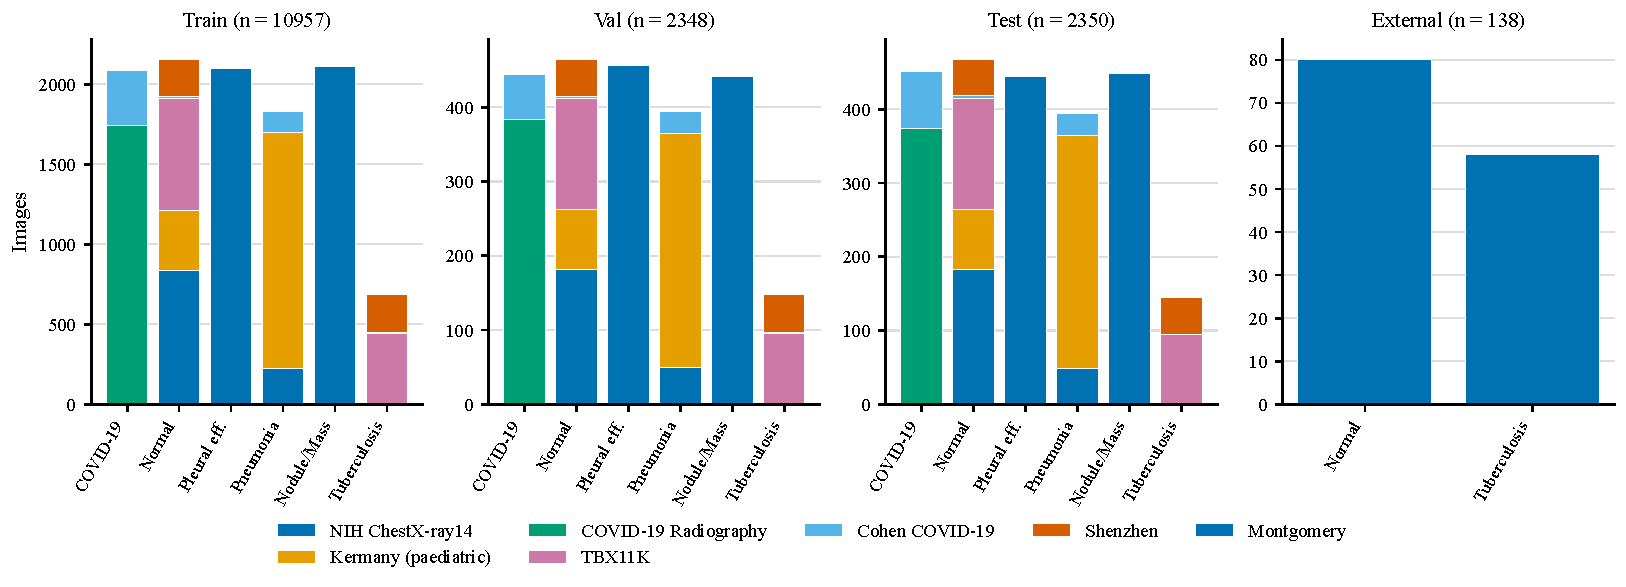
\includegraphics[width=\linewidth]{fig_dataset_composition.pdf}
\caption{Images per class and source in the training, validation and test splits of the dataset build used for the reported model (\RDatasetBuild). Generated from the build manifest.}
\label{fig:composition}
\end{figure}

\subsection{External cohort}
The Montgomery County set contains 138 frontal radiographs from a United States county TB control programme: 80 normal and 58 with TB manifestations~\cite{jaeger2014two,candemir2014lung}. It shares no source with the development data, was never used for training or checkpoint selection and was evaluated once per run; Section~\ref{sec:design} gives the caveat that run~2 was started after run~1's external results had been seen. It contains only normal and TB images, so it tests whether the classifier separates abnormal from normal radiographs from an unseen hospital, and whether it names TB correctly; it does not test six-class accuracy.

\section{Methods}
\label{sec:methods}

Fig.~\ref{fig:pipeline} summarises the pipeline. The same preprocessing functions are called by the dataset builder, the training and evaluation code and the web service, so that training and serving cannot drift apart.

\begin{figure}[t]
\centering
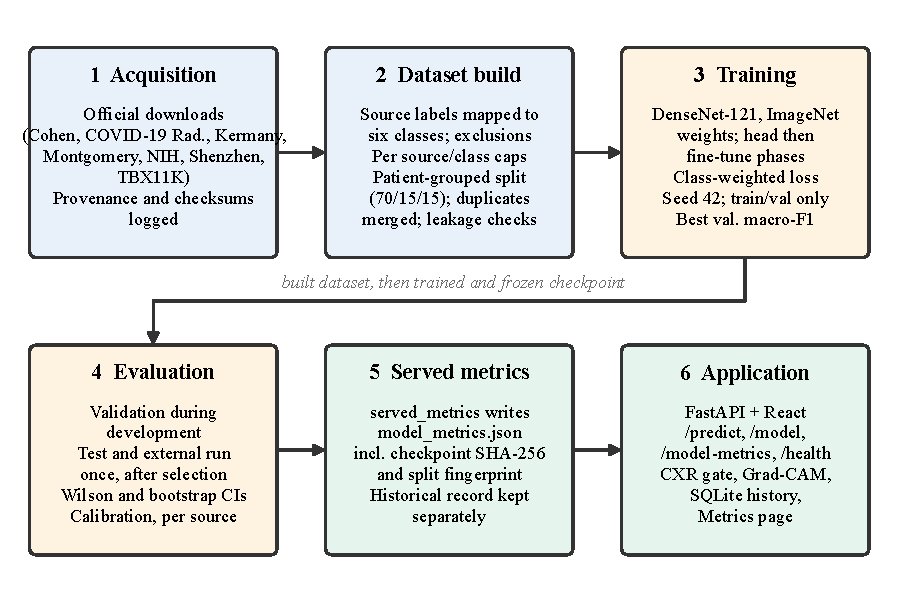
\includegraphics[width=\linewidth]{fig_pipeline.pdf}
\caption{End-to-end pipeline: acquisition with provenance, dataset build (labelling rules, caps, patient- and duplicate-grouped split, leakage checks), training with checkpoint selection on validation, once-only evaluation on the internal test split and the external cohort, and the metrics file served by the application.}
\label{fig:pipeline}
\end{figure}

\subsection{Preprocessing}
\label{sec:preproc}
Each image is decoded to an 8-bit, three-channel RGB array $I$ (grey-level images are replicated across channels and any alpha channel is dropped). Four deterministic steps follow, illustrated in Fig.~\ref{fig:preproc}.

\paragraph{Gaussian pre-blur} A $3\times3$ Gaussian kernel with $\sigma_1=0.8$ suppresses pixel-level noise and compression artefacts before contrast enhancement, which would otherwise amplify them:
\begin{equation}
I_1 = G_{\sigma_1} * I,\qquad
G_{\sigma}(x,y)=\frac{1}{Z_\sigma}\exp\!\left(-\frac{x^2+y^2}{2\sigma^2}\right),
\label{eq:blur}
\end{equation}
where $*$ denotes two-dimensional convolution applied per channel and $Z_\sigma$ normalises the discrete kernel to unit sum.

\paragraph{Contrast-limited adaptive histogram equalisation} $I_1$ is converted to the CIE $L^*a^*b^*$ colour space and CLAHE~\cite{pizer1987adaptive,zuiderveld1994contrast} is applied to the lightness channel $L$ only. The image is divided into an $8\times8$ grid of tiles. In tile $t$ with $M_t$ pixels and histogram $h_t(v)$ over $V=256$ grey levels, the histogram is clipped at
\begin{equation}
\beta_t = \max\!\left(1,\ \left\lfloor c\,\frac{M_t}{V}\right\rfloor\right),\qquad c=2.0,
\end{equation}
and the clipped excess $E_t=\sum_v \max(0,h_t(v)-\beta_t)$ is redistributed uniformly, $\tilde h_t(v)=\min(h_t(v),\beta_t)+E_t/V$. The tile mapping is the scaled cumulative distribution
\begin{equation}
T_t(v)=\frac{V-1}{M_t}\sum_{u=0}^{v}\tilde h_t(u),
\label{eq:clahe}
\end{equation}
and the output value of each pixel is the bilinear interpolation of the mappings of the four nearest tile centres, which avoids block artefacts. Clipping limits the slope of $T_t$ and therefore the amplification of noise in homogeneous regions. The enhanced $L$ channel is recombined with the unchanged $a^*,b^*$ channels and converted back to RGB, giving $I_2$.

\paragraph{Gaussian low-pass filter} A second Gaussian filter with $\sigma_2=1.0$ and kernel size $k=2\lceil 3\sigma_2\rceil+1=7$ is applied, $I_3=G_{\sigma_2}*I_2$. In the frequency domain the filter attenuates spatial frequency $(u,v)$ (in cycles per pixel) by
\begin{equation}
H(u,v)=\exp\!\left(-2\pi^2\sigma_2^2\,(u^2+v^2)\right),
\label{eq:lowpass}
\end{equation}
so that high-frequency texture enhanced by CLAHE, together with fine-grained acquisition artefacts, is damped. The value $\sigma_2=1.0$ was chosen in the earlier V5 work by comparing ten candidate filters (Gaussian $\sigma\in\{1,2,3\}$, ideal and Butterworth low-pass filters at three cut-offs each, and no filter) on the V5 validation split with a fixed baseline checkpoint and keeping the highest validation macro-F1. It was not re-tuned on V6; a run without the three filters is described in Section~\ref{sec:followup}.

\paragraph{Resizing and normalisation} $I_3$ is resized to $224\times224$ pixels with Lanczos interpolation (8$\times$8 support) and each channel $c$ is normalised with the ImageNet statistics,
\begin{equation}
x_c=\frac{I_{4,c}/255-\mu_c}{s_c},\qquad \boldsymbol\mu=(0.485,0.456,0.406),\ \ \mathbf{s}=(0.229,0.224,0.225).
\end{equation}
The three filters operate at the native resolution of each source image, before resizing. The same anatomy acquired at a different resolution therefore receives a different effective filter; this is a known limitation (Section~\ref{sec:limitations}). The builder caches the $224\times224$ result of the first four steps for each image, keyed by the SHA-256 of the raw file.

\begin{figure}[t]
\centering
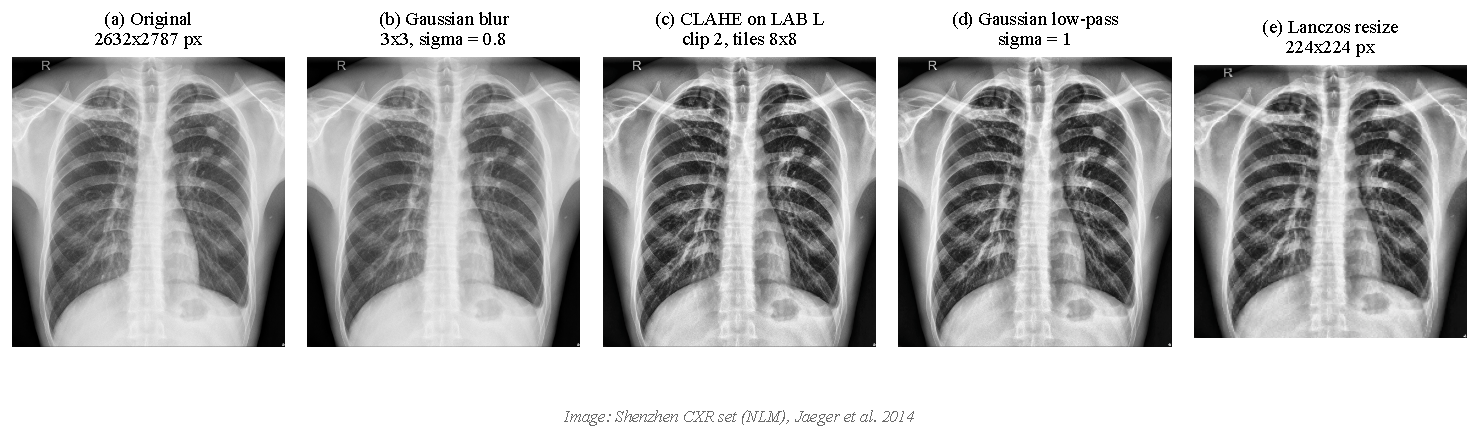
\includegraphics[width=\linewidth]{fig_preprocessing.pdf}
\caption{One radiograph through the preprocessing chain: input, Gaussian pre-blur ($\sigma_1=0.8$), CLAHE on the lightness channel (clip limit 2.0, $8\times8$ tiles), Gaussian low-pass ($\sigma_2=1.0$) and resizing to $224\times224$.}
\label{fig:preproc}
\end{figure}

\paragraph{Augmentation} During training only, each image is flipped horizontally with probability 0.5 and rotated by an angle drawn uniformly from $[-10^\circ,10^\circ]$ with reflected borders. Horizontal flipping reverses cardiac laterality; whether to keep it should be decided on validation in future work.

\subsection{Network}
The classifier (Fig.~\ref{fig:model}) is a DenseNet-121~\cite{huang2017densely} initialised with ImageNet weights~\cite{deng2009imagenet}, as in earlier chest radiograph work~\cite{rajpurkar2017chexnet}. Let $\phi(\mathbf{x})\in\mathbb{R}^{7\times7\times1024}$ be the final feature map of the backbone. The head computes
\begin{equation}
\mathbf{z}=\mathrm{GAP}(\phi(\mathbf{x})),\quad
\mathbf{a}=\mathrm{Dropout}_{0.3}\!\left(\mathrm{ReLU}\!\left(W_1\,\mathrm{BN}(\mathbf{z})+\mathbf{b}_1\right)\right),\quad
\mathbf{p}=\mathrm{softmax}(W_2\mathbf{a}+\mathbf{b}_2),
\label{eq:head}
\end{equation}
with global average pooling (GAP), batch normalisation (BN), $W_1\in\mathbb{R}^{256\times1024}$ and $W_2\in\mathbb{R}^{6\times256}$. The output $\mathbf{p}\in\Delta^5$ is the softmax score vector over the six classes, and the predicted class is $\hat y=\arg\max_k p_k$. The softmax scores are not calibrated probabilities of disease.

\begin{figure}[t]
\centering
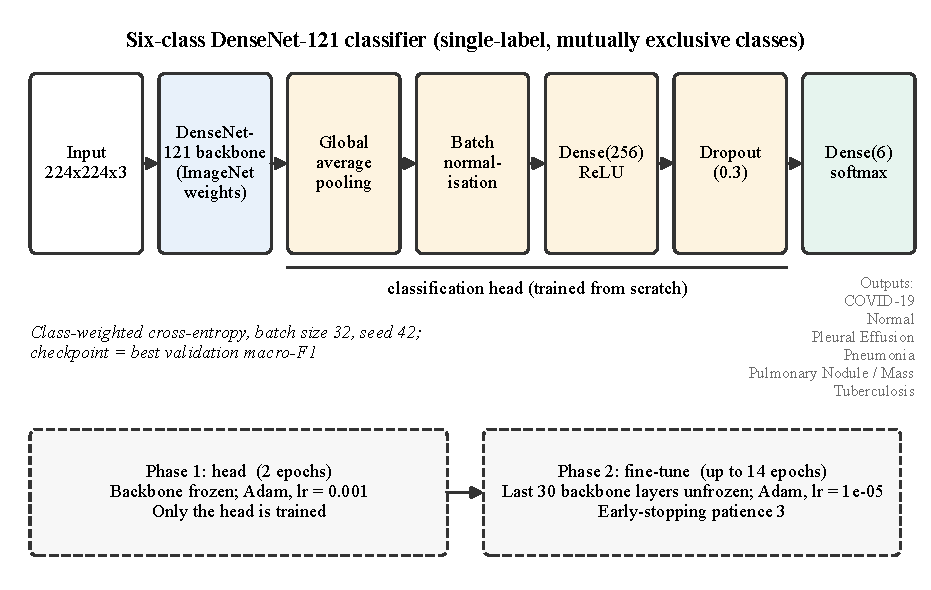
\includegraphics[width=\linewidth]{fig_model_architecture.pdf}
\caption{Model: DenseNet-121 backbone, global average pooling, batch normalisation, a 256-unit ReLU layer, dropout 0.3 and a six-way softmax. Phase~1 trains the head with the backbone frozen; phase~2 also unfreezes the last 30 backbone layers.}
\label{fig:model}
\end{figure}

\subsection{Loss with class weights}
The classes are imbalanced (Table~\ref{tab:builds}). With $n$ training images, $K=6$ classes and $n_k$ training images in class $k$, each training example receives the balanced weight
\begin{equation}
w_k=\frac{n}{K\,n_k},
\label{eq:weights}
\end{equation}
so that every class contributes the same total weight. The loss on a mini-batch $\mathcal{B}$ is the weighted categorical cross-entropy
\begin{equation}
\mathcal{L}(\theta)=\frac{1}{|\mathcal{B}|}\sum_{i\in\mathcal{B}} w_{y_i}\left(-\log p_{y_i}(\mathbf{x}_i;\theta)\right).
\label{eq:loss}
\end{equation}

\subsection{Two-phase optimisation}
Training uses Adam~\cite{kingma2015adam} with mini-batches of 32 and seed \RSeed{} for all random number generators. In phase~1 (two epochs) the backbone is frozen and only the head is trained with learning rate $10^{-3}$. In phase~2 the last 30 layers of the backbone are unfrozen and training continues with learning rate $10^{-5}$ until one of three conditions holds: three consecutive epochs without an improvement of validation macro-F1 (early stopping), the configured maximum number of phase-2 epochs, or a wall-clock budget. Batch-normalisation layers inside the unfrozen block are trained together with the convolutional layers. Each epoch is one pass over the training split.

\subsection{Checkpoint selection}
After every epoch the model is evaluated on the validation split and the checkpoint with the highest validation macro-F1 is kept, with validation macro ROC-AUC as tie-breaker:
\begin{equation}
e^\star=\arg\max_{e}\ \left(\mathrm{F1}^{\text{val}}_{\text{macro}}(e),\ \mathrm{AUC}^{\text{val}}_{\text{macro}}(e)\right)\quad\text{(lexicographic)}.
\end{equation}
Macro-F1 was chosen over accuracy because it weights the small COVID-19 and Tuberculosis classes equally with the large ones. Neither the internal test split nor the external cohort influences training or selection.

\subsection{Evaluation metrics}
\label{sec:metrics}
For class $k$ on a set of $N$ images, let $\mathrm{TP}_k$, $\mathrm{FP}_k$, $\mathrm{FN}_k$ and $\mathrm{TN}_k$ be the one-vs-rest counts derived from the $6\times6$ confusion matrix $C$ (rows true, columns predicted). Then
\begin{gather}
\mathrm{Prec}_k=\frac{\mathrm{TP}_k}{\mathrm{TP}_k+\mathrm{FP}_k},\quad
\mathrm{Rec}_k=\frac{\mathrm{TP}_k}{\mathrm{TP}_k+\mathrm{FN}_k},\quad
\mathrm{Spec}_k=\frac{\mathrm{TN}_k}{\mathrm{TN}_k+\mathrm{FP}_k},\quad
\mathrm{F1}_k=\frac{2\,\mathrm{Prec}_k\,\mathrm{Rec}_k}{\mathrm{Prec}_k+\mathrm{Rec}_k},\\
\mathrm{Acc}=\frac{1}{N}\sum_k C_{kk},\qquad
\mathrm{F1}_{\text{macro}}=\frac{1}{K}\sum_{k=1}^{K}\mathrm{F1}_k,\qquad
\mathrm{F1}_{\text{weighted}}=\sum_{k=1}^{K}\frac{N_k}{N}\,\mathrm{F1}_k ,
\end{gather}
where $N_k$ is the number of images of class $k$; macro precision and macro recall are defined analogously. A ratio with a zero denominator is reported as zero.

\paragraph{Ranking metrics} For class $k$, with positive set $P_k$ (images of class $k$) and negative set $Q_k$ (all others), the one-vs-rest ROC-AUC is the Mann--Whitney statistic on the score $p_k$,
\begin{equation}
\mathrm{AUC}_k=\frac{1}{|P_k||Q_k|}\sum_{i\in P_k}\sum_{j\in Q_k}\left(\mathbb{1}[p_{ik}>p_{jk}]+\tfrac12\,\mathbb{1}[p_{ik}=p_{jk}]\right),
\end{equation}
and macro ROC-AUC is the unweighted mean over the six classes. The precision--recall area (PR-AUC) is the average precision $\mathrm{AP}_k=\sum_n(R_n-R_{n-1})P_n$ over the thresholds $n$ of the ranked scores, with $P_n$ and $R_n$ the precision and recall at the $n$-th threshold; macro PR-AUC is the unweighted mean.

\paragraph{Calibration} The expected calibration error~\cite{naeini2015obtaining,guo2017calibration} is computed on the top-class score $\hat p_i=\max_k p_{ik}$ with $M=15$ equal-width bins $B_m$ on $[0,1]$:
\begin{equation}
\mathrm{ECE}=\sum_{m=1}^{M}\frac{|B_m|}{N}\left|\mathrm{acc}(B_m)-\mathrm{conf}(B_m)\right|,
\label{eq:ece}
\end{equation}
where $\mathrm{acc}(B_m)$ is the fraction of correct predictions and $\mathrm{conf}(B_m)$ the mean top-class score in bin $m$. No calibration map was fitted.

\paragraph{Confidence intervals} For a proportion $\hat\pi=x/n$ (accuracy, per-class recall, external sensitivity and specificity) we report the Wilson score interval~\cite{wilson1927probable} with $z=1.96$:
\begin{equation}
\frac{\hat\pi+\frac{z^2}{2n}\pm z\sqrt{\frac{\hat\pi(1-\hat\pi)}{n}+\frac{z^2}{4n^2}}}{1+\frac{z^2}{n}} .
\label{eq:wilson}
\end{equation}
For accuracy, macro-F1 and macro ROC-AUC we also compute a percentile bootstrap interval~\cite{efron1994introduction}: $B=2{,}000$ resamples of the $N$ test images drawn with replacement (seed 42), the metric $\hat\theta^{*}_b$ recomputed on each, and the interval $[\hat\theta^{*}_{(2.5)},\hat\theta^{*}_{(97.5)}]$ given by the 2.5th and 97.5th percentiles. For macro ROC-AUC only resamples that contain all six classes are used. These intervals describe sampling variation of the test set for a fixed model; they do not include variation due to training (seed, data order), which was not measured.

\subsection{External binary task}
\label{sec:exttask}
Montgomery contains only normal and TB radiographs, so the six-class metrics do not apply. We define a prediction as \emph{abnormal} if $\hat y\neq\text{Normal}$ and report
\begin{equation}
\mathrm{Sens}=\frac{\#\{\text{TB scans predicted abnormal}\}}{\#\{\text{TB scans}\}},\qquad
\mathrm{Spec}=\frac{\#\{\text{normal scans predicted Normal}\}}{\#\{\text{normal scans}\}},
\end{equation}
each with its Wilson interval, the exact Tuberculosis recall $\#\{\text{TB scans predicted Tuberculosis}\}/\#\{\text{TB scans}\}$, the ROC-AUC of the abnormality score $s=1-p_{\text{Normal}}$, and the full table of predicted classes for normal and TB scans. Sensitivity is never reported without specificity: a model that calls every image abnormal has a sensitivity of one. No threshold was tuned on the external cohort or on the internal test split.

\subsection{Grad-CAM}
Grad-CAM~\cite{selvaraju2017gradcam} maps are computed on the last ReLU activation of the backbone for the predicted class, upsampled to the input size and overlaid on the preprocessed image. They are used only for qualitative inspection; they show which regions influenced the class score, not radiological reasoning. Saliency methods including Grad-CAM have been found to fail localisation and sanity criteria on chest radiographs~\cite{arun2021assessing}, so we draw no conclusion from them about what the model has learned. The examples shown were selected by a rule fixed before any heatmap was viewed: for each class, the correctly classified test image whose top-class score is the median among the correctly classified test images of that class.
% Source of the rule: lungai/evaluation/make_figures.py::fig_gradcam_examples.

\subsection{Source-identifiability probe}
\label{sec:probe}
Per-source accuracy (Section~\ref{sec:res-source}) cannot separate a source effect from a difference in case mix. As a more direct control we asked whether the source collection of an image can be predicted from the features the classifier uses, both overall and among images of a single class. A classifier that recognises collections, as shown for hospital systems by Zech et~al.~\cite{zech2018variable}, could exploit any class--source association~\cite{degrave2021ai,geirhos2020shortcut}.

From build~2 we drew, separately for every (source, class) pair, at most 150 images of the training split and at most 100 images of the test split (fixed random seed), giving \RProbeNTrain{} probe-training and \RProbeNTest{} probe-test images; because the probe-training and probe-test images come from different splits, they are patient- and duplicate-separated as described in Section~\ref{sec:materials}. Each cached, preprocessed image (Section~\ref{sec:preproc}) was mapped to the 1024-dimensional GAP vector $\mathbf{z}$ of Eq.~\eqref{eq:head} by two frozen feature extractors: (i) DenseNet-121 with ImageNet weights only, which has learned nothing from this project, and (ii) the backbone of the selected model. Features were standardised with the mean and standard deviation of the probe-training set, and a multinomial logistic regression (L2 penalty with inverse strength $C=1$, class weights inversely proportional to source frequency) was fitted to predict the \emph{source}, not the disease. On the probe-test images we report the balanced accuracy, the mean over sources of the per-source recall, whose chance level is $1/S$ for $S$ sources; we report it over all images and within each class that has at least two sources in the probe-test set (Normal, Pneumonia, COVID-19 and Tuberculosis). Pleural Effusion and Nodule/Mass come from NIH only and cannot be probed within class. The probe does not influence any model or selection decision.
% Implementation: lungai/evaluation/source_probe.py (--per-group-train 150 --per-group-test 100 --seed 0); output artifacts/data_quality/source_probe_v6_build_002.json.

A high within-class balanced accuracy means that source information is linearly available in the features, so that a classifier \emph{could} separate classes by source style. It does not show that the trained classifier \emph{does} so; we therefore treat the probe as indirect evidence, to be read together with the per-source and external results.

\section{Experimental design}
\label{sec:design}

\subsection{Two dataset builds and two runs}
The experiment consists of two training runs with the identical model, preprocessing and optimisation settings (Section~\ref{sec:methods}), one per dataset build (Section~\ref{sec:builds}):
\begin{itemize}
\item \textbf{Run 1} trained on build~1 (five sources, every COVID-19 image from the COVID-19 image data collection, Tuberculosis almost entirely from Shenzhen), with at most eight phase-2 epochs.
\item \textbf{Run 2} trained on build~2, which adds TBX11K and the COVID-19 Radiography Database so that COVID-19 and Tuberculosis each come from two sources, with at most fourteen phase-2 epochs and a wall-clock budget.
\end{itemize}
Both added sources were part of the original data design, with labelling rules fixed before any training, but had not finished downloading when build~1 was made. Adding them is a data intervention, not a tuning step, and it does not use the internal test split or the external cohort for any parameter. However, run~2 was started after run~1's test and external results had been seen, and those results bear directly on the question that build~2 addresses (single-source classes). The external cohort therefore cannot be considered fully untouched by the overall research process. The timeline was as follows. Run~1's external results were produced at about 09:28 on 2026-11-03. Run~2 was started at about 10:07 the same day. The rule for choosing between the runs (Section~\ref{sec:selection}) was written after run~2 had started but before any of run~2's validation, test or external results existed. We state this explicitly; a new external cohort would be needed for a strictly prospective evaluation of the selected model (Section~\ref{sec:limitations}).

\subsection{Fair comparison of the two runs}
\label{sec:selection}
Each run selected its own epoch on its own build's validation split. Because the two validation splits differ in composition, their scores are not comparable, and the test and external results may not be used to choose between runs. A selection rule was therefore fixed in advance and recorded in the repository before run~2's results existed (it was not registered with any external body), and kept unchanged in the project record.
% Source: docs/data/run_selection_protocol.md (written 2026-11-03 ~12:00); implementation lungai/evaluation/compare_runs.py -> artifacts/evaluation_reports/run_comparison.json. An image belongs to the \emph{common selection set} if (i) it is in the validation split of build~1 or build~2; (ii) it does not occur in the training or test split of either build, checked both by exact file (MD5) and by patient key (source plus patient identifier where the identity is genuine or derived from the file name, otherwise the file's SHA-256); and (iii) its label is the same in both builds where it appears in both. Montgomery images are never included.

The primary criterion is macro-F1 over the six classes on this set; the run with the higher value is selected. If the difference is below 0.01, run~1 (the model already integrated and verified in the application) is kept unless run~2's macro ROC-AUC is higher by at least 0.01. Accuracy, macro ROC-AUC, per-class recall and the same metrics restricted to the four sources present in both builds are reported alongside, because run~2 has an in-distribution advantage on the TBX11K and COVID-19 Radiography images. An exact McNemar test on the paired predictions is reported as a descriptive statistic only: with one seed per run, no claim is made that one training recipe is better in general. The run not selected is reported as a secondary experiment, labelled as such.

\subsection{Follow-up runs: seed variability and preprocessing ablation}
\label{sec:followup}
Before run~2 had been evaluated and before the two runs were compared, three further runs on the build of the selected run were fixed in the project record (Table~\ref{tab:followup}). They are trained one after another, because parallel training does not fit in 8~GB of memory.
% Source: docs/data/run_selection_protocol.md, "Follow-up runs" (fixed 2026-11-03 ~15:00).

\begin{table}[t]
\centering
\caption{Follow-up runs, fixed before the run comparison. All use the build, architecture, class weights, optimiser schedule and early-stopping patience of the selected run.}
\label{tab:followup}
\small
\begin{tabular}{@{}llll@{}}
\toprule
Run & Seed & Change from the selected recipe & Purpose \\
\midrule
Run 3 & 43 & none & Seed-to-seed variability \\
Run 4 & 44 & none & Seed-to-seed variability \\
Run 5 & \RSeed{} (as run 2) & no Gaussian pre-blur, CLAHE or low-pass filter & Preprocessing ablation \\
\bottomrule
\end{tabular}
\end{table}

Runs 3 and 4 differ from the selected run only in the seed of all random number generators (which control, for example, the initialisation of the head, the data order, augmentation and dropout). Run 5 uses the seed of the selected run but a cache of images resized and normalised without the three filters of Section~\ref{sec:preproc}, with the same manifest and the same split, so that the only difference is the filtering. Because the selected run may in principle have been ended by its wall-clock budget rather than its epoch limit, each follow-up run gets a phase-2 epoch limit equal to the number of phase-2 epochs that the selected run actually completed and a wall-clock budget well above the expected duration, so that all runs receive the same schedule; early stopping (patience 3) still applies. Each run is evaluated once on validation, test and external data.
% Ablation cache: scripts/data/make_ablation_build.py --variant no_filters.

Seed variability is reported as the mean, sample standard deviation, minimum and maximum over the selected run and runs 3 and 4. The ablation is a single run (one seed) and is read against that spread. The served model remains the one chosen by the rule in Section~\ref{sec:selection}; the follow-up runs do not replace it, because choosing the best of several seeds on test or external results would be selection on the evaluation sets.
% Aggregation: lungai/evaluation/aggregate_seeds.py -> artifacts/evaluation_reports/multi_seed_summary.json -> \RMS... and \RAbl... macros.

\subsection{Once-only evaluation}
For each run, the internal test split and the external cohort were evaluated exactly once, after the checkpoint had been fixed on validation. No threshold, preprocessing parameter or training setting was changed after those evaluations for that run. Per-class and per-source results on the test split are reported but were not acted on, with the exception discussed in the previous paragraphs (the decision to add sources for build~2, which did not use test images for any parameter).

\subsection{Analyses}
The following analyses are reported for the selected model: (a) overall internal metrics with confidence intervals; (b) per-class precision, recall, specificity, F1 and ROC-AUC, and the confusion matrix; (c) accuracy and class recall within each source of the internal test split, because the overall figure depends on the source mix and a source that is the only provider of a class can be recognised by its image style; (d) calibration (reliability diagram and ECE); (e) the external binary task, including the full table of predicted classes for Montgomery's normal and TB scans; (f) the comparison of runs on the common selection set; (g) the source-identifiability probe (Section~\ref{sec:probe}); (h) seed variability and the preprocessing ablation (Section~\ref{sec:followup}); and (i) qualitative Grad-CAM maps.

\subsection{Compute environment and reproducibility}
Training and evaluation ran on a laptop CPU with 8~GB of memory under Windows, using Python~3.12, TensorFlow~2.16 and Keras~3; TensorFlow has no GPU support on native Windows, so no GPU was used. Because of this, runs 1 and 2 are single seeds (\RSeed), seed variability is limited to the three runs of Section~\ref{sec:followup}, and every run is bounded by an epoch limit or a wall-clock budget; the run reported in Section~\ref{sec:results} trained for \REpochsTrained{} epochs and its selected checkpoint is from epoch \RSelectedEpoch. Every training run writes a metadata record containing the code version, a full configuration snapshot, the manifest SHA-256 and split fingerprint, the seed, library versions and platform, per-epoch history, the class weights and the checkpoint SHA-256. Every evaluation report repeats the checkpoint SHA-256 (\texttt{\RCheckpointShort\ldots} for the reported model, version \RModelVersion), the manifest SHA-256 and the split fingerprint. All numbers in this paper are generated from those reports into a macro file; none was typed by hand. The images themselves cannot be redistributed under the source licences; the repository contains the rules, the builder, the provenance logs and the checksums needed to rebuild the identical dataset from the official sources.

\confirm{Describe here any use of AI-assisted tools in developing the software and analysis pipeline, as required by the Elsevier policy for use of AI in the research process; see the declaration at the end of the manuscript.}

\section{Results}
\label{sec:results}

Unless stated otherwise, all values in this section are from the selected model (version \RModelVersion, dataset build \RDatasetBuild, checkpoint \texttt{\RCheckpointShort\ldots}, seed \RSeed) and come from a single training run. Differences of a few percentage points between classes, sources or runs are within the range that seed-to-seed variation could produce and should not be read as established; the seed runs are reported in Section~\ref{sec:res-seeds}.

Run~2 was selected by the rule of Section~\ref{sec:selection}, because its macro-F1 on the common selection set was higher than that of run~1 (\RCmpRunTwoMacroFOne\% versus \RCmpRunOneMacroFOne\%); much of this advantage lies on sources that only run~2 trained on (Section~\ref{sec:res-runs}).

\subsection{Training}
Fig.~\ref{fig:curves} shows the training loss and the validation accuracy, macro-F1 and macro ROC-AUC per epoch. The run completed its full schedule of \REpochsTrained{} epochs (two head-only epochs followed by all configured phase-2 epochs); neither early stopping nor the wall-clock budget ended it. The checkpoint from epoch \RSelectedEpoch, the last epoch, had the highest validation macro-F1 and was selected, with validation accuracy \RValAcc\%, macro-F1 \RValMacroFOne\% and macro ROC-AUC \RValMacroAUC. The validation curve was still rising slightly at the end, so the run had not clearly plateaued; whether longer training would change the results was not tested.

\begin{figure}[t]
\centering
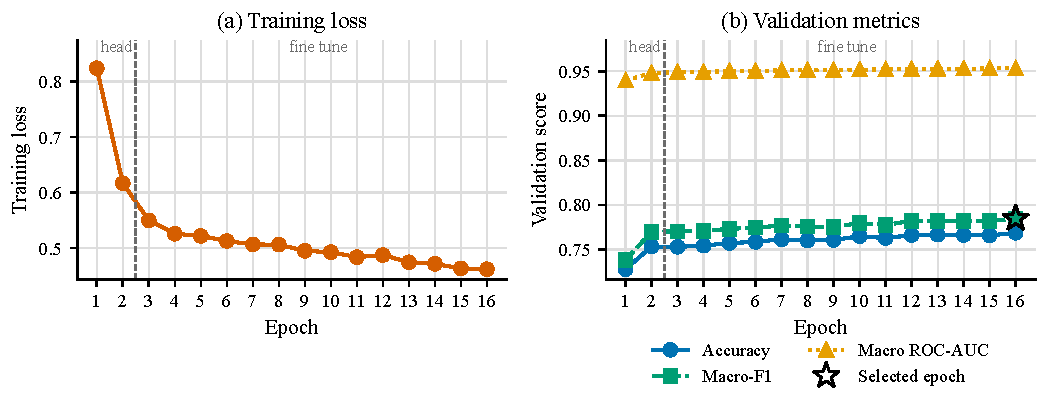
\includegraphics[width=\linewidth]{fig_training_curves.pdf}
\caption{Training loss and validation accuracy, macro-F1 and macro ROC-AUC per epoch for the selected run. Epochs 1--2: head only (backbone frozen); later epochs: last 30 backbone layers unfrozen.}
\label{fig:curves}
\end{figure}

\subsection{Overall internal performance}
Table~\ref{tab:overall} gives the validation and test results. On the internal test split ($N=\RNTest$), accuracy was \RTestAcc\% (Wilson 95\% CI \RTestAccLo--\RTestAccHi\%; percentile-bootstrap 95\% CI \RTestAccBootLo--\RTestAccBootHi\%), macro-F1 \RTestMacroFOne\%, weighted F1 \RTestWeightedFOne\%, macro precision \RTestMacroPrecision\%, macro recall \RTestMacroRecall\%, macro ROC-AUC \RTestMacroAUC{} and macro PR-AUC \RTestMacroPRAUC. Validation and test values are close (accuracy \RValAcc\% and \RTestAcc\%, macro ROC-AUC \RValMacroAUC{} and \RTestMacroAUC), so checkpoint selection on validation did not produce a visible optimistic bias for this split. The macro ROC-AUC is much higher than the threshold metrics: within the internal distribution the scores rank images of a class above images of other classes well, but the arg-max decision is wrong for about one test image in four, and most of these errors fall among a few classes (Section~\ref{sec:res-perclass}). A high ranking metric on internal data says nothing about whether the arg-max class is right on data from another hospital (Section~\ref{sec:res-ext}).

\begin{table}[t]
\centering
\caption{Overall results of the selected model. Validation was used for checkpoint selection; the test split was evaluated once. Accuracy CI: Wilson 95\%.}
\label{tab:overall}
\small
\begin{tabular}{@{}lrrrrr@{}}
\toprule
Split & $N$ & Accuracy (\%) & Macro-F1 (\%) & Macro ROC-AUC & Macro PR-AUC \\
\midrule
Validation & \RNVal & \RValAcc & \RValMacroFOne & \RValMacroAUC & -- \\
Test & \RNTest & \RTestAcc{} (\RTestAccLo--\RTestAccHi) & \RTestMacroFOne & \RTestMacroAUC & \RTestMacroPRAUC \\
\bottomrule
\end{tabular}
\end{table}

\subsection{Per-class performance}
\label{sec:res-perclass}
Table~\ref{tab:perclass} reports per-class metrics on the test split, Fig.~\ref{fig:cm} the confusion matrix, Fig.~\ref{fig:roc} the one-vs-rest ROC curves and Fig.~\ref{fig:perclass} precision, recall and F1 with recall confidence intervals.
The strongest classes by F1 were COVID-19 (\RFOneCovid\%), Tuberculosis (\RFOneTB\%) and Pneumonia (\RFOnePneumonia\%); COVID-19 and Tuberculosis also had the highest ROC-AUC (\RAUCCovid{} and \RAUCTB). The weakest were Pulmonary Nodule/Mass (F1 \RFOneNodule\%, ROC-AUC \RAUCNodule) and Normal (F1 \RFOneNormal\%). Most errors in the confusion matrix lie among Normal, Pleural Effusion and Nodule/Mass: Normal radiographs predicted as Nodule/Mass, and Nodule/Mass and Pleural Effusion confused with each other in both directions. Pleural Effusion and Nodule/Mass come only from NIH ChestX-ray14, whose labels were mined from radiology reports by natural language processing rather than read from the images; label noise and the subtlety of small nodules are both plausible contributors, which this study cannot separate. For the two small classes, high ROC-AUC did not come with low precision: COVID-19 and Tuberculosis had precision \RPrecisionCovid\% and \RPrecisionTB\%. The lowest precision was for Nodule/Mass (\RPrecisionNodule\%), the class into which most Normal errors fell.
% Confusion pattern: artifacts/evaluation_reports/model_metrics.json, internal_test.metrics.confusion_matrix (also fig_confusion_matrix).

\begin{table}[t]
\centering
\caption{Per-class results on the internal test split (one-vs-rest). Precision, recall, specificity and F1 in \%.}
\label{tab:perclass}
\small
\begin{tabular}{@{}lrrrrrr@{}}
\toprule
Class & Support & Precision & Recall & Specificity & F1 & ROC-AUC \\
\midrule
COVID-19              & \RSupportCovid     & \RPrecisionCovid     & \RRecallCovid     & \RSpecificityCovid     & \RFOneCovid     & \RAUCCovid \\
Normal                & \RSupportNormal    & \RPrecisionNormal    & \RRecallNormal    & \RSpecificityNormal    & \RFOneNormal    & \RAUCNormal \\
Pleural Effusion      & \RSupportEffusion  & \RPrecisionEffusion  & \RRecallEffusion  & \RSpecificityEffusion  & \RFOneEffusion  & \RAUCEffusion \\
Pneumonia             & \RSupportPneumonia & \RPrecisionPneumonia & \RRecallPneumonia & \RSpecificityPneumonia & \RFOnePneumonia & \RAUCPneumonia \\
Pulmonary Nodule/Mass & \RSupportNodule    & \RPrecisionNodule    & \RRecallNodule    & \RSpecificityNodule    & \RFOneNodule    & \RAUCNodule \\
Tuberculosis          & \RSupportTB        & \RPrecisionTB        & \RRecallTB        & \RSpecificityTB        & \RFOneTB        & \RAUCTB \\
\midrule
Macro average         & \RNTest            & \RTestMacroPrecision & \RTestMacroRecall & --                     & \RTestMacroFOne & \RTestMacroAUC \\
\bottomrule
\end{tabular}
\end{table}

\begin{figure}[t]
\centering
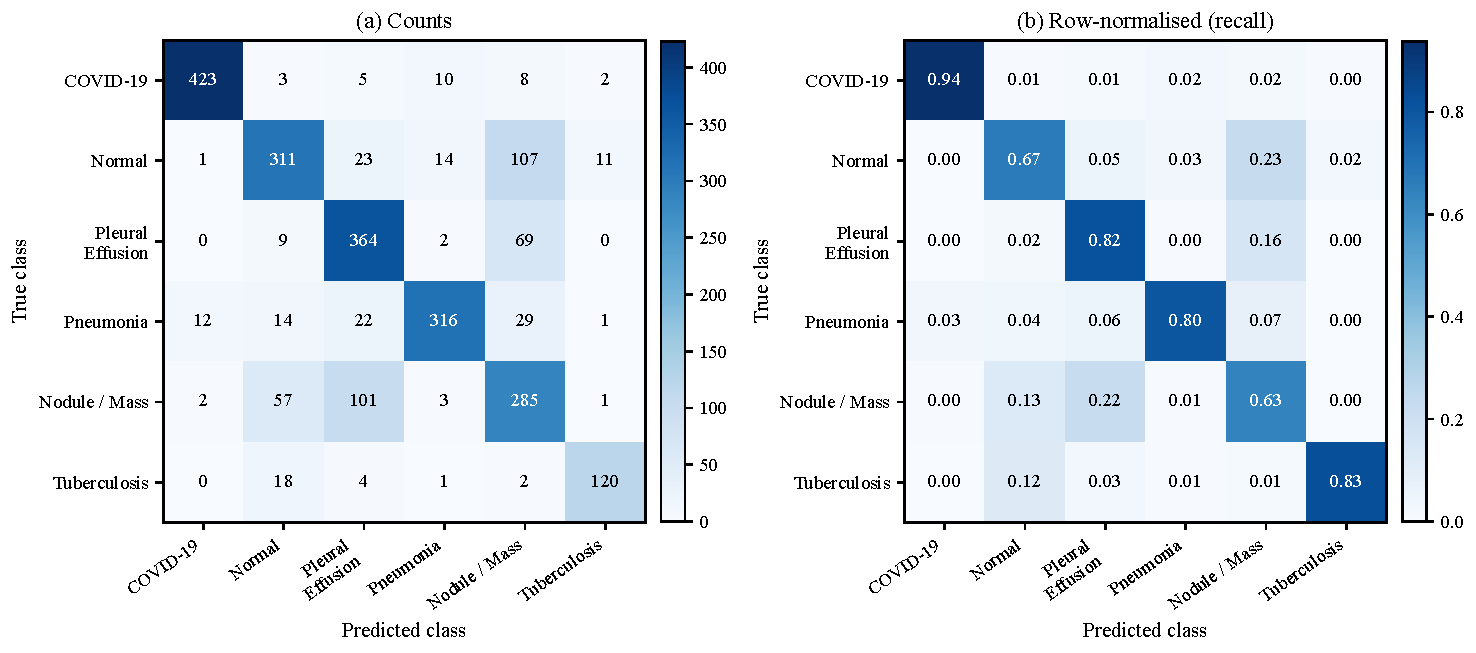
\includegraphics[width=\linewidth]{fig_confusion_matrix.pdf}
\caption{Confusion matrix on the internal test split: counts (left) and row-normalised (right). Rows: true class; columns: predicted class.}
\label{fig:cm}
\end{figure}

\begin{figure}[t]
\centering
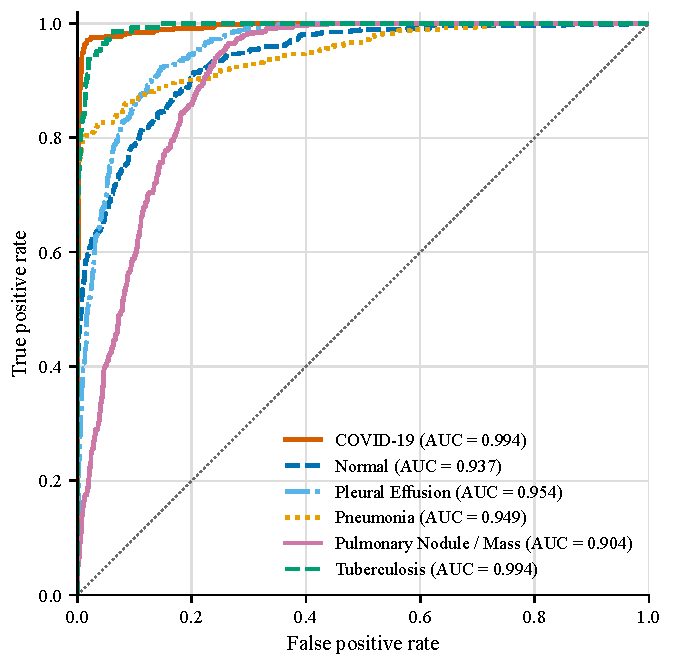
\includegraphics[width=0.8\linewidth]{fig_roc_curves.pdf}
\caption{One-vs-rest ROC curves per class on the internal test split, with per-class area under the curve.}
\label{fig:roc}
\end{figure}

\begin{figure}[t]
\centering
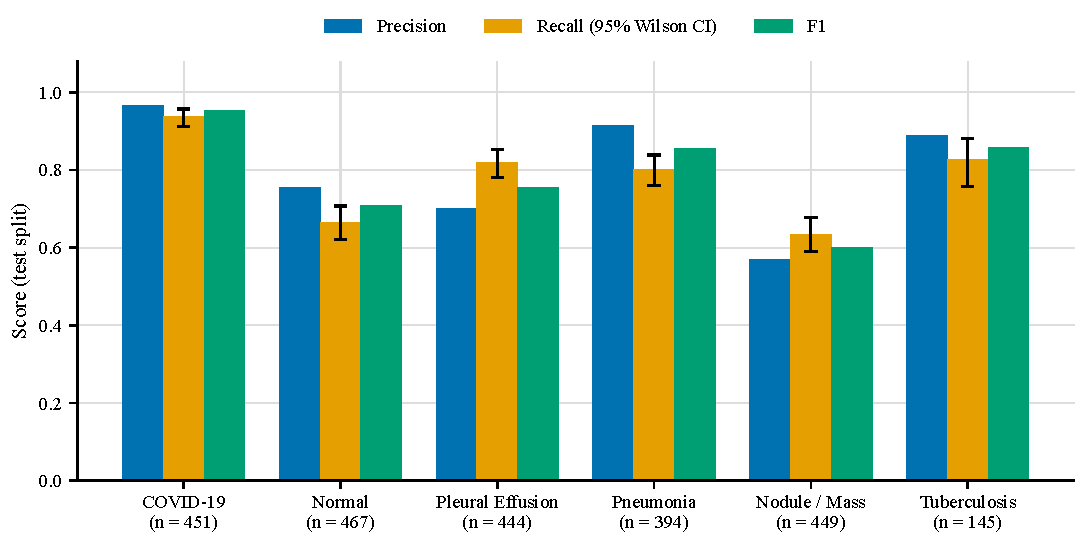
\includegraphics[width=\linewidth]{fig_per_class_metrics.pdf}
\caption{Precision, recall and F1 per class on the internal test split; error bars show Wilson 95\% confidence intervals for recall.}
\label{fig:perclass}
\end{figure}

\subsection{Performance by source}
\label{sec:res-source}
Table~\ref{tab:persource} and Fig.~\ref{fig:persource} give test accuracy within each source. Because several classes are supplied by one or two sources only, these values show how strongly the internal result depends on which collection an image came from; they are not measures of the quality of a source or of the diagnostic difficulty of its images.

\begin{table}[t]
\centering
\caption{Accuracy of the selected model within each source of the internal test split. ``Classes'' lists the classes that the source contributes to the test split.}
\label{tab:persource}
\small
\begin{tabular}{@{}llrr@{}}
\toprule
Source & Classes & $N$ & Accuracy (\%) \\
\midrule
NIH ChestX-ray14 & Normal, Effusion, Pneumonia, Nodule/Mass & \RSrcNNIH & \RSrcAccNIH \\
Kermany (paediatric) & Normal, Pneumonia & \RSrcNKermany & \RSrcAccKermany \\
COVID-19 Radiography Database & COVID-19 & \RSrcNCovidRad & \RSrcAccCovidRad \\
TBX11K & Normal, Tuberculosis & \RSrcNTBXk & \RSrcAccTBXk \\
Shenzhen & Normal, Tuberculosis & \RSrcNShenzhen & \RSrcAccShenzhen \\
COVID-19 image data collection & COVID-19, Normal, Pneumonia, TB & \RSrcNCohen & \RSrcAccCohen \\
\bottomrule
\end{tabular}
\end{table}

Accuracy ranged from \RSrcAccCohen\% (COVID-19 image data collection) to \RSrcAccCovidRad\% (COVID-19 Radiography Database), a source that contributes a single class. Kermany (paediatric Normal and Pneumonia) and TBX11K (Normal and Tuberculosis) reached \RSrcAccKermany\% and \RSrcAccTBXk\%, whereas NIH, which supplies four classes including the two NIH-only classes, reached \RSrcAccNIH\%. The overall test accuracy of \RTestAcc\% is a weighted mixture of these values and would change with the source mix. The same class was also recognised very differently depending on its source: Normal radiographs from NIH were called Normal far less often than Normal radiographs from Kermany, Shenzhen or TBX11K. This pattern is consistent with source-specific appearance contributing to the decisions, but per-source accuracy alone cannot separate a source effect from differences in case mix; Section~\ref{sec:res-probe} addresses this more directly.
% Within-source class recall: artifacts/evaluation_reports/model_metrics.json, internal_test.per_source.<source>.recall_by_class (not in the macro file).

\begin{figure}[t]
\centering
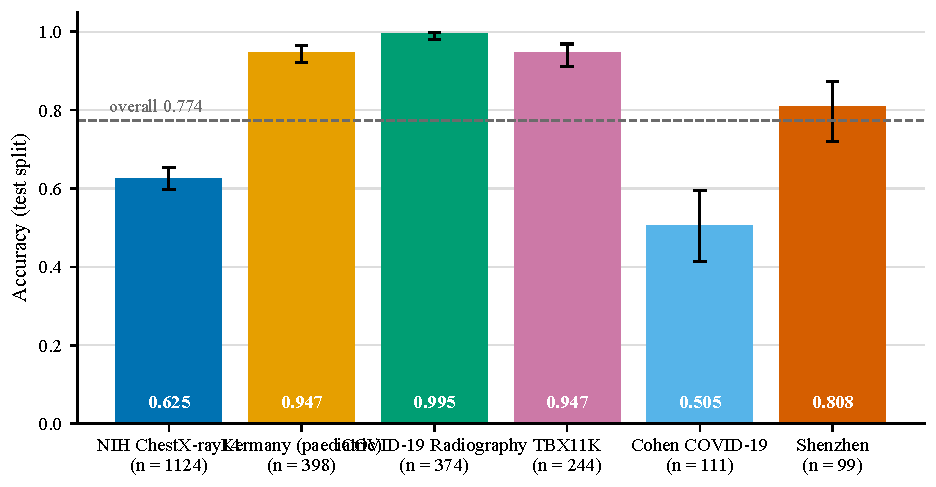
\includegraphics[width=0.85\linewidth]{fig_per_source.pdf}
\caption{Accuracy on the internal test split within each source. A source that is the only provider of a class can be recognised by its image style rather than by disease, so these values are not comparable with one another as measures of diagnostic difficulty.}
\label{fig:persource}
\end{figure}

\subsection{Source-identifiability probe}
\label{sec:res-probe}
Table~\ref{tab:probe} gives the balanced accuracy with which the linear probe of Section~\ref{sec:probe} predicted the source of the \RProbeNTest{} probe-test images. With ImageNet features, which contain nothing learned from this project, the source was identified with balanced accuracy \RProbeImgBalAcc\% across \RProbeImgNSources{} sources (chance \RProbeImgChance\%). The source remained identifiable within single classes: among Normal images \RProbeImgWithinNormal\% across \RProbeImgWithinNormalNSources{} sources (chance \RProbeImgWithinNormalChance\%), among Tuberculosis images \RProbeImgWithinTB\% (chance \RProbeImgWithinTBChance\%), among Pneumonia images \RProbeImgWithinPneumonia\% (chance \RProbeImgWithinPneumoniaChance\%) and among COVID-19 images \RProbeImgWithinCovid\% (chance \RProbeImgWithinCovidChance\%). Features from the trained model's backbone gave nearly identical values (\RProbeMdlBalAcc\% overall). This is expected: fine-tuning changed only the last 17 weighted layers of the backbone, so its features remain close to the ImageNet features (verified by comparing the weights).

\begin{table}[t]
\centering
\caption{Source-identifiability probe: balanced accuracy (\%) of a logistic regression predicting the source collection from frozen 1024-dimensional features, on \RProbeNTest{} probe-test images (\RProbeNTrain{} probe-training images). ``Within'' rows use only images of that class. Chance is $1/S$ for $S$ sources.}
\label{tab:probe}
\small
\begin{tabular}{@{}lrrrr@{}}
\toprule
Images & Sources & Chance & ImageNet features & Trained backbone \\
\midrule
All classes & \RProbeImgNSources & \RProbeImgChance & \RProbeImgBalAcc & \RProbeMdlBalAcc \\
Within Normal & \RProbeImgWithinNormalNSources & \RProbeImgWithinNormalChance & \RProbeImgWithinNormal & \RProbeMdlWithinNormal \\
Within Tuberculosis & \RProbeImgWithinTBNSources & \RProbeImgWithinTBChance & \RProbeImgWithinTB & \RProbeMdlWithinTB \\
Within Pneumonia & \RProbeImgWithinPneumoniaNSources & \RProbeImgWithinPneumoniaChance & \RProbeImgWithinPneumonia & \RProbeMdlWithinPneumonia \\
Within COVID-19 & \RProbeImgWithinCovidNSources & \RProbeImgWithinCovidChance & \RProbeImgWithinCovid & \RProbeMdlWithinCovid \\
\bottomrule
\end{tabular}
\end{table}

Because each source supplies a different subset of classes (Table~\ref{tab:persource}), source and class are confounded in this benchmark, and the probe shows that source information is linearly available in the very features on which the classifier's head operates. A source shortcut is therefore possible. The probe does not show that the classifier uses it; that conclusion would need an intervention such as leave-one-source-out training, which was not performed. We treat the probe as indirect evidence and interpret it only together with the per-source results above, the external breakdown (Section~\ref{sec:res-ext}) and the Grad-CAM examples (Section~\ref{sec:res-gradcam}).

\subsection{Calibration}
The expected calibration error on the test split was \RTestECE{} (15 equal-width bins; Eq.~\eqref{eq:ece}); Fig.~\ref{fig:calib} shows the reliability diagram. The highest-score bin holds the largest share of test images and lies close to the diagonal. In several bins of the middle score range accuracy is somewhat below the mean score, a mild over-confidence, and incorrect predictions have a clearly lower mean top-class score than correct ones. A low ECE on the internal test split does not imply calibrated scores on data from another hospital, where, as shown below, the arg-max class is often wrong. No calibration map was fitted, and the 0.5 ``inconclusive'' threshold used by the application has not been validated.
% Source: artifacts/evaluation_reports/model_metrics.json, internal_test.metrics.calibration (bins, mean_confidence_correct, mean_confidence_incorrect).

\begin{figure}[t]
\centering
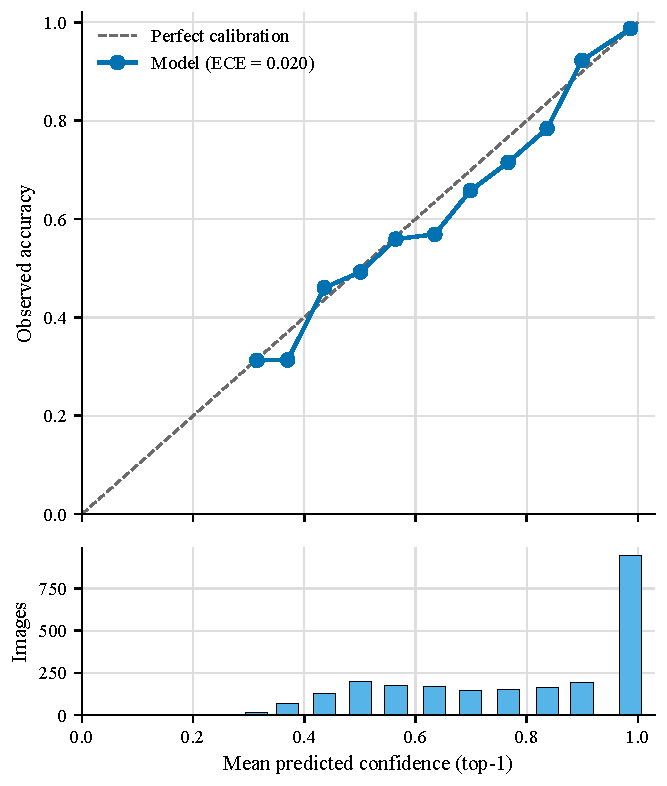
\includegraphics[width=0.6\linewidth]{fig_calibration.pdf}
\caption{Reliability diagram on the internal test split: accuracy versus mean top-class softmax score in 15 equal-width bins. The diagonal is perfect calibration.}
\label{fig:calib}
\end{figure}

\subsection{External cohort}
\label{sec:res-ext}
Table~\ref{tab:external} and Fig.~\ref{fig:external} give the results on the Montgomery cohort ($N=\RNExternal$). Of the \RExtSensN{} TB radiographs, \RExtSensK{} were predicted as some class other than Normal (sensitivity \RExtSens\%, 95\% CI \RExtSensLo--\RExtSensHi\%); of the \RExtSpecN{} normal radiographs, \RExtSpecK{} were predicted Normal (specificity \RExtSpec\%, 95\% CI \RExtSpecLo--\RExtSpecHi\%). The ROC-AUC of the abnormality score $1-p_{\text{Normal}}$ was \RExtAUC. Exactly \RExtTBK{} of \RExtTBN{} TB radiographs (\RExtTB\%) were assigned the Tuberculosis class. The model assigned COVID-19 to \RExtCovidCalls{} of the \RNExternal{} external radiographs, although the cohort contains no COVID-19 cases.

Fig.~\ref{fig:external} shows where the errors went. Most Montgomery radiographs, normal and TB alike, were assigned Pneumonia or Pulmonary Nodule/Mass, and some TB radiographs Pleural Effusion. The high sensitivity is therefore not TB detection: the TB scans were called abnormal, but with a disease the cohort does not contain, while the internal Tuberculosis recall was \RRecallTB\%. The low specificity means that the model would flag most healthy patients from this hospital as abnormal. That the ROC-AUC of $1-p_{\text{Normal}}$ (\RExtAUC) is well above chance while specificity is low indicates that the scores still order TB scans above normal scans to some degree, but the decision boundary learned on the development sources does not transfer.

Run~1, which had seen COVID-19 only from the COVID-19 image data collection, behaved differently on the same cohort, also evaluated once: it assigned COVID-19 to \RRunOneExtCovidCalls{} of the \RNExternal{} Montgomery radiographs, called \RRunOneExtSpecK{} of the \RExtSpecN{} normal radiographs Normal and named \RRunOneExtTBK{} of the \RExtTBN{} TB radiographs Tuberculosis.
With build~2, which added TBX11K, the COVID-19 Radiography Database and two further NIH archives at once, the COVID-19 calls on Montgomery fell from \RRunOneExtCovidCalls{} to \RExtCovidCalls. This is consistent with, but does not prove, run~1 having associated the appearance of its single COVID-19 source with the class; build~2 changed several sources together, so the change cannot be attributed to one of them. The external errors did not become correct, however: they moved to other abnormal classes, specificity was lower than run~1's, and Tuberculosis was still not recognised, although Tuberculosis in build~2 also comes from two sources. The internal gains of run~2 did not translate into better external specificity or any TB recognition. These are single-seed observations on one small cohort.

\begin{table}[t]
\centering
\caption{External cohort (Montgomery County; binary normal vs TB; evaluated once). ``Abnormal'' means any predicted class other than Normal. CIs: Wilson 95\%.}
\label{tab:external}
\small
\begin{tabular}{@{}lrr@{}}
\toprule
Quantity & Count & \% (95\% CI) \\
\midrule
TB scans predicted abnormal (sensitivity) & \RExtSensK/\RExtSensN & \RExtSens{} (\RExtSensLo--\RExtSensHi) \\
Normal scans predicted Normal (specificity) & \RExtSpecK/\RExtSpecN & \RExtSpec{} (\RExtSpecLo--\RExtSpecHi) \\
TB scans predicted Tuberculosis (exact TB recall) & \RExtTBK/\RExtTBN & \RExtTB \\
All scans predicted COVID-19 & \RExtCovidCalls/\RNExternal & -- \\
ROC-AUC of $1-p_{\text{Normal}}$ & \multicolumn{2}{r}{\RExtAUC} \\
\bottomrule
\end{tabular}
\end{table}

\begin{figure}[t]
\centering
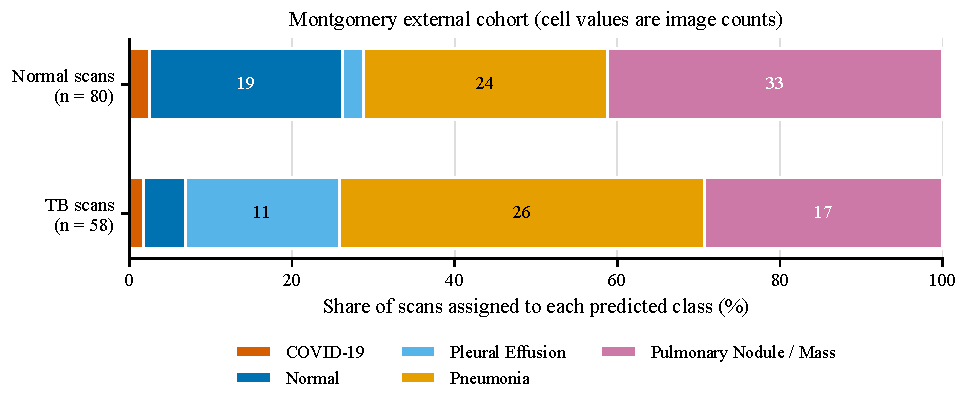
\includegraphics[width=\linewidth]{fig_external_breakdown.pdf}
\caption{Predicted class for the normal (left) and TB (right) radiographs of the external Montgomery cohort. The cohort contains no COVID-19, Pleural Effusion, Pneumonia or Nodule/Mass cases.}
\label{fig:external}
\end{figure}

\subsection{Comparison of run 1 and run 2}
\label{sec:res-runs}
Table~\ref{tab:runs} compares the two runs on the common selection set defined in Section~\ref{sec:selection} and reports each run's once-only test and external results for completeness. Test rows are not comparable between runs, because the two builds have different test splits, and neither test nor external rows were used for selection.

\begin{table}[t]
\centering
\caption{Comparison of run~1 (build~1) and run~2 (build~2). Selection used only the macro-F1 on the common selection set. Shared sources: NIH, Kermany, Shenzhen and the COVID-19 image data collection, on which both runs trained. Single seed per run; the McNemar test is descriptive. Percentages except ROC-AUC.}
\label{tab:runs}
\small
\begin{tabular}{@{}lll@{}}
\toprule
Quantity & Run 1 & Run 2 \\
\midrule
Common set: $N$ & \multicolumn{2}{c}{\RCmpN} \\
Common set: macro-F1 (selection criterion) & \RCmpRunOneMacroFOne & \RCmpRunTwoMacroFOne \\
Common set: macro ROC-AUC & \RCmpRunOneMacroAUC & \RCmpRunTwoMacroAUC \\
Common set: accuracy & \RCmpRunOneAcc & \RCmpRunTwoAcc \\
Shared sources only: $N$ & \multicolumn{2}{c}{\RCmpRunOneSharedN} \\
Shared sources only: macro-F1 & \RCmpRunOneSharedMacroFOne & \RCmpRunTwoSharedMacroFOne \\
Shared sources only: macro ROC-AUC & \RCmpRunOneSharedMacroAUC & \RCmpRunTwoSharedMacroAUC \\
Shared sources only: accuracy & \RCmpRunOneSharedAcc & \RCmpRunTwoSharedAcc \\
Exact McNemar test, all common images & \multicolumn{2}{c}{\RCmpMcNemarB{} vs \RCmpMcNemarC{} discordant; $p=\RCmpMcNemarP$} \\
\midrule
Own test split: $N$ & \RRunOneTestN & \RNTest \\
Own test split: accuracy / macro-F1 & \RRunOneTestAcc{} / \RRunOneTestMacroFOne & \RTestAcc{} / \RTestMacroFOne \\
Own test split: macro ROC-AUC & \RRunOneTestMacroAUC & \RTestMacroAUC \\
External: sensitivity / specificity & \RRunOneExtSensK/\RExtSensN{} / \RRunOneExtSpecK/\RExtSpecN & \RExtSensK/\RExtSensN{} / \RExtSpecK/\RExtSpecN \\
External: ROC-AUC of $1-p_{\text{Normal}}$ & \RRunOneExtAUC & \RExtAUC \\
External: exact TB recall; COVID-19 calls & \RRunOneExtTBK/\RExtTBN; \RRunOneExtCovidCalls & \RExtTBK/\RExtTBN; \RExtCovidCalls \\
\midrule
Selected & & \checkmark{} (\RCmpSelected) \\
\bottomrule
\end{tabular}
\end{table}
% McNemar: first count = run 1 right and run 2 wrong; second = run 1 wrong and run 2 right.

By the rule of Section~\ref{sec:selection}, which was fixed in advance and recorded in the repository before run~2's results existed (run~2 itself was started after run~1's external results had been seen), run~2 was selected: its macro-F1 on the \RCmpN{} common images was \RCmpRunTwoMacroFOne\% against \RCmpRunOneMacroFOne\% for run~1, with accuracy \RCmpRunTwoAcc\% against \RCmpRunOneAcc\% and macro ROC-AUC \RCmpRunTwoMacroAUC{} against \RCmpRunOneMacroAUC. Of the paired predictions that differed in correctness, \RCmpMcNemarB{} were right for run~1 only and \RCmpMcNemarC{} for run~2 only (exact McNemar $p=\RCmpMcNemarP$), a statistic we report as descriptive.

\textbf{This comparison favours run~2 by construction, and the size of the gap should not be read as the effect of a better training recipe.} The common set includes TBX11K and COVID-19 Radiography images, which are in-distribution for run~2 and unseen for run~1. Restricted to the \RCmpRunOneSharedN{} common images from the four sources both runs trained on, the two runs had almost the same accuracy (\RCmpRunOneSharedAcc\% and \RCmpRunTwoSharedAcc\%) and the same macro ROC-AUC (\RCmpRunOneSharedMacroAUC{} and \RCmpRunTwoSharedMacroAUC), and the macro-F1 gap was much smaller (\RCmpRunOneSharedMacroFOne\% and \RCmpRunTwoSharedMacroFOne\%). Much of run~2's advantage therefore lies on the sources that only run~2 trained on. The selection rule was fixed before run~2's results were known, but run~2 itself was started after run~1's external results had been seen (Section~\ref{sec:design}). On the external cohort, the one data set that neither run trained on, run~2 removed run~1's COVID-19 calls but did not improve specificity (Section~\ref{sec:res-ext}). With one seed per run, none of these differences is evidence that one recipe is better in general.

\subsection{Seed variability}
\label{sec:res-seeds}
Table~\ref{tab:seeds} reports the selected run and the two follow-up seeds of Section~\ref{sec:followup}, each evaluated once on the test split and the external cohort. \pending{seed variability: size of the seed-to-seed spread of test accuracy, macro-F1, macro ROC-AUC, external specificity and exact TB recall; whether the selected run lies inside the spread; which earlier statements (class, source and run differences) are smaller than the spread. Use \texttt{\textbackslash RMS...} macros only}.

\begin{table}[t]
\centering
\caption{Seed variability of the selected configuration (build \RDatasetBuild). Test values in \%, except ROC-AUC; external specificity and exact Tuberculosis recall in \%. Mean $\pm$ sample SD over the three runs. The served model is run~2 regardless of these results.}
\label{tab:seeds}
\small
\begin{tabular}{@{}llrrrrr@{}}
\toprule
Run & Seed & Test acc. & Macro-F1 & Macro ROC-AUC & Ext. specificity & Ext. TB recall \\
\midrule
Run 2 (selected) & \RSeed & \RTestAcc & \RTestMacroFOne & \RTestMacroAUC & \RExtSpec & \RExtTB \\
% Run 2 row = \RMSRunOne... (Seed, TestAcc, TestMacroFOne, TestMacroAUC, ExtSens, ExtSpec, ExtTB); values identical to the macros used here.
Run 3 & 43 % \RMSRunTwoSeed
  & \pending{} % \RMSRunTwoTestAcc
  & \pending{} % \RMSRunTwoTestMacroFOne
  & \pending{} % \RMSRunTwoTestMacroAUC
  & \pending{} % \RMSRunTwoExtSpec
  & \pending{} % \RMSRunTwoExtTB
  \\
Run 4 & 44 % \RMSRunThreeSeed
  & \pending{} % \RMSRunThreeTestAcc
  & \pending{} % \RMSRunThreeTestMacroFOne
  & \pending{} % \RMSRunThreeTestMacroAUC
  & \pending{} % \RMSRunThreeExtSpec
  & \pending{} % \RMSRunThreeExtTB
  \\
\midrule
Mean $\pm$ SD & --
  & \pending{} % \RMSTestAccMean $\pm$ \RMSTestAccSD
  & \pending{} % \RMSTestMacroFOneMean $\pm$ \RMSTestMacroFOneSD
  & \pending{} % \RMSTestMacroAUCMean $\pm$ \RMSTestMacroAUCSD
  & \pending{} % \RMSExtSpecMean $\pm$ \RMSExtSpecSD
  & \pending{} % \RMSExtTBMean $\pm$ \RMSExtTBSD
  \\
\bottomrule
\end{tabular}
\end{table}
% Fill the Mean +/- SD row with \RMSTestAccMean $\pm$ \RMSTestAccSD, \RMSTestMacroFOneMean $\pm$ \RMSTestMacroFOneSD,
% \RMSTestMacroAUCMean $\pm$ \RMSTestMacroAUCSD, \RMSExtSpecMean $\pm$ \RMSExtSpecSD, \RMSExtTBMean $\pm$ \RMSExtTBSD
% (also available: \RMS<metric>Min/Max, \RMSExtSensMean/SD, \RMSExtAUCMean/SD, \RMSNRuns, \RMSSeeds).
% Per-run macros (after aggregation): \RMSRun<One|Two|Three><Seed|TestAcc|TestMacroFOne|TestMacroAUC|ExtSens|ExtSpec|ExtTB>, One = run 2, Two = run 3, Three = run 4.

\subsection{Preprocessing ablation}
\label{sec:res-ablation}
Table~\ref{tab:ablation} compares the selected run, trained with the full filtering chain, with run~5, trained with the same seed, data and schedule but without the Gaussian pre-blur, CLAHE and low-pass filter. \pending{ablation: direction and size of the differences on test and external data, read against the seed spread of Table~\ref{tab:seeds}; no claim that the filtering helps or harms unless the difference clearly exceeds that spread. Use \texttt{\textbackslash RAbl...} macros only}.

\begin{table}[t]
\centering
\caption{Preprocessing ablation: full chain (run~2) versus no filtering (run~5), same seed (\RSeed), build, split and schedule. One run each; compare differences with the seed spread in Table~\ref{tab:seeds}. Percentages except ROC-AUC.}
\label{tab:ablation}
\small
\begin{tabular}{@{}lrr@{}}
\toprule
Quantity & Run 2 (full chain) & Run 5 (no filters) \\
\midrule
Test accuracy & \RTestAcc & \pending{} \\
Test macro-F1 & \RTestMacroFOne & \pending{} \\
Test macro ROC-AUC & \RTestMacroAUC & \pending{} \\
External sensitivity & \RExtSens & \pending{} \\
External specificity & \RExtSpec & \pending{} \\
External exact TB recall & \RExtTB & \pending{} \\
\bottomrule
\end{tabular}
\end{table}
% Fill run-5 cells with \RAblTestAcc, \RAblTestMacroFOne, \RAblTestMacroAUC, \RAblExtSens, \RAblExtSpec, \RAblExtTB.

\subsection{Grad-CAM examples}
\label{sec:res-gradcam}
Fig.~\ref{fig:gradcam} shows Grad-CAM maps for one test image per class, chosen by the rule fixed before any heatmap was viewed (Section~\ref{sec:methods}): the correctly classified image with the median top-class score of its class. In these examples the COVID-19 and Normal heatmaps concentrate on the neck and trachea, the shoulders and the image borders rather than the lung fields; the Nodule/Mass and Tuberculosis heatmaps fall inside the lung fields; and the Pneumonia example, a paediatric image from the Kermany collection, is diffuse. With one image per class these maps are illustrative only. Attention outside the lungs for COVID-19 and Normal is consistent with acquisition or source cues contributing to those decisions, but it does not establish it, and saliency maps on chest radiographs are themselves unreliable~\cite{arun2021assessing}.

\begin{figure}[t]
\centering
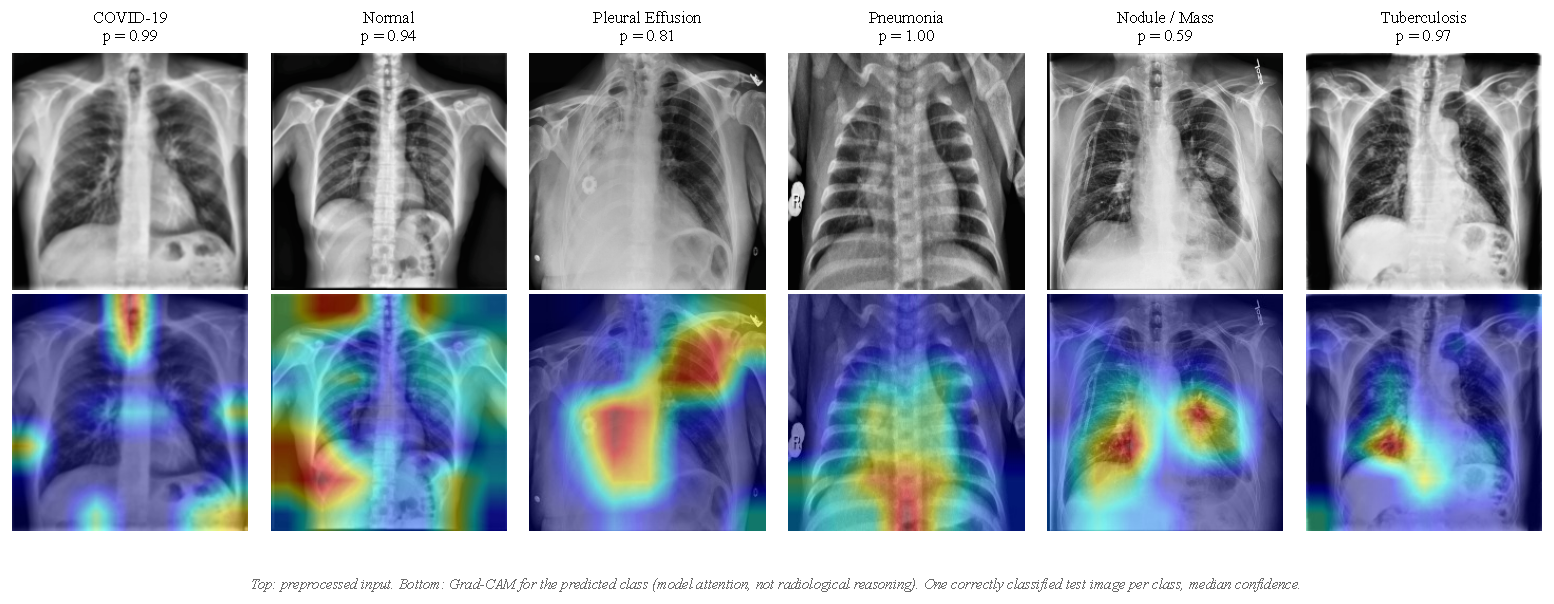
\includegraphics[width=\linewidth]{fig_gradcam_examples.pdf}
\caption{Grad-CAM maps for the predicted class on one correctly classified test radiograph per class, each the image with the median top-class score among the correct predictions of its class (rule fixed before viewing). The maps show which regions influenced the class score; they do not show radiological reasoning.}
\label{fig:gradcam}
\end{figure}

\section{Discussion}
\label{sec:discussion}

\subsection{Internal versus external behaviour}
With patient- and duplicate-grouped splits and no proxy labels, a standard DenseNet-121 reached an internal test accuracy of \RTestAcc\% and a macro ROC-AUC of \RTestMacroAUC. On radiographs from a hospital it had never seen, the same model flagged \RExtSensK/\RExtSensN{} TB scans as abnormal but called only \RExtSpecK/\RExtSpecN{} normal scans Normal, and it named \RExtTBK/\RExtTBN{} TB scans Tuberculosis, although its internal Tuberculosis recall was \RRecallTB\%. Its external predictions were dominated by Pneumonia and Nodule/Mass, classes the cohort does not contain. The internal results therefore overstate the behaviour of this model on an unseen hospital by a wide margin, and they do so even though the usual leakage paths were closed: leakage control is necessary for a credible internal estimate, but it does not make that estimate a measure of generalisation.

Four observations point to source confounding as one reason, and we stress that each is indirect. First, the benchmark is confounded by design: classes come from different subsets of sources, and the source of an image can be predicted from frozen ImageNet features with \RProbeImgBalAcc\% balanced accuracy (chance \RProbeImgChance\%), and still within a single class, for example \RProbeImgWithinNormal\% among Normal images (chance \RProbeImgWithinNormalChance\%). Source information is thus linearly available in the features on which the classifier's head operates. Second, internal accuracy varies widely between sources (Table~\ref{tab:persource}), and Normal images were recognised much less often when they came from NIH than from other sources. Third, run~1, whose only COVID-19 source was the COVID-19 image data collection, called about half of the Montgomery radiographs COVID-19 (\RRunOneExtCovidCalls{} of \RNExternal);
 when build~2 added a large second COVID-19 source, run~2 almost stopped doing so, which is what one would expect if run~1 had linked the appearance of that single source with the class. Fourth, the pre-specified Grad-CAM examples for COVID-19 and Normal highlight the neck, shoulders and image borders rather than the lungs. None of these shows that the classifier relies on source cues; together they make that explanation plausible, and a causal test (leave-one-source-out training, masking of regions outside the lungs) remains to be done.

Adding sources did not close the external gap. Run~2's errors on Montgomery moved from COVID-19 to Pneumonia and Nodule/Mass instead of becoming correct, its external specificity was lower than run~1's, and Tuberculosis was still not recognised although it now comes from two sources (Shenzhen and TBX11K). Adding a second source per class changed where the external errors went rather than removing the external gap. On the common selection set run~2 was clearly better, but most of that advantage lies on the sources only run~2 trained on: on the four shared sources the two runs had nearly the same accuracy (Section~\ref{sec:res-runs}). These are single-seed observations; Section~\ref{sec:res-seeds} reports how much seeds alone change the results.

Finally, the external ROC-AUC of the abnormality score (\RExtAUC) is well above chance while specificity is low, just as the internal macro ROC-AUC is much higher than internal accuracy. Ranking metrics reward scores that order positives above negatives, whatever the absolute level; on a new hospital, a shift of the scores towards ``abnormal'' can leave the ranking partly intact and still move most normal images across the arg-max boundary. A model that is to be deployed at a new site would at least need its operating point re-established there, and a high ranking metric on internal data is not evidence that this is unnecessary. We do not compare these numbers with those of other studies, which used different data and splits.

Independently of the final numbers, the design of the evaluation determines what can be concluded. Internal test images share sources, acquisition devices, post-processing and, for some sources, populations with the training images. For a class that is supplied by one collection, the internal test set cannot distinguish a model that recognises the disease from one that recognises the collection~\cite{zech2018variable,degrave2021ai,maguolo2020critic}. The external cohort breaks this link for two classes only (Normal and Tuberculosis), and it does so in a deliberately weak way: it asks whether normal radiographs from an unseen hospital are called Normal and whether TB radiographs are called abnormal and, more strictly, Tuberculosis. Reporting the full table of predicted classes on this cohort, rather than a single sensitivity, is what makes a shortcut visible: an abnormal prediction counts towards sensitivity even if the predicted disease is one the cohort does not contain.

\subsection{What the audit of the earlier pipeline showed}
\label{sec:disc-audit}
The V5 pipeline that preceded this work is the clearest illustration of why these controls matter. V5 pooled eight public sources, several of them obtained from third-party redistributions, into 10,547 images, and its partitions were built incrementally across dataset versions. Its canonical model recorded an internal test accuracy of \RVFiveAcc\% on $N=\RVFiveN$ images. A retrospective audit of the manifests, ingestion code and recorded results found the following.
\begin{itemize}
\item \textbf{Patient leakage.} Patient tokens recoverable from Kermany file names showed that 154 of the 1,570 internal test images (9.8\%) belonged to patients who also had images in the training split. A further 8,478 images had no real patient identity, so their separation could not be checked at all.
\item \textbf{Proxy and latent labels.} 1,395 Pneumonia labels (about half of the class) were TBX11K images labelled ``sick but non-TB'', whose cause is not specified; 124 Tuberculosis labels were latent TB; and 1,440 of 1,467 VinDr-CXR images used as single-label examples carried two or more findings.
\item \textbf{Degenerate external behaviour.} On the Montgomery cohort, every recorded V5 variant (five training paradigms, including two domain-adaptation methods) flagged essentially every TB radiograph as abnormal but called none of the normal radiographs Normal (specificity \RVFiveExtSpecK/\RVFiveExtSpecN). A sensitivity quoted alone would have suggested a perfect screening tool; with specificity it describes a model that never outputs Normal on that hospital.
\item \textbf{Possible contamination of the external cohort.} One V5 TB source is described as containing Montgomery images. A content check (MD5 and perceptual hash) found no match, but it also found no match for Shenzhen images that the archive is described as containing, so the check cannot rule the overlap out. V6 does not use that archive.
\item \textbf{Reporting errors.} A comparison table in earlier drafts differed from the result files in 13 of 35 cells, all in the direction of making comparator runs look worse, and three figures captioned as the canonical model showed a baseline run. The canonical checkpoint itself was lost, so ROC-AUC and calibration could not be re-verified.
\end{itemize}
None of these defects is unusual in isolation; together they produced an internal accuracy that said little about the model. V6 was designed so that each defect is either removed (proxy labels, aggregated archives, per-image splitting of patients with known identity) or explicitly measured and reported (unknown identity, near-duplicates, external specificity, per-source performance). The V5 numbers are not comparable with V6: the data, the splits and the label definitions differ.

\subsection{Implications for multi-source benchmark design}
From the audit and the rebuild we draw the following recommendations, which do not depend on the final V6 numbers.
\begin{enumerate}
\item \textbf{Acquire from official sources and log provenance.} Third-party redistributions rename files, drop patient identifiers and silently merge collections; the overlap between a redistributed TB archive and our external cohort could not be resolved for this reason. A per-file record of URL, size and SHA-256 makes a dataset rebuildable without redistributing images.
\item \textbf{Fix labelling rules before training, and label from the source's own labels only.} Rules that map ``abnormal, not TB'' to ``pneumonia'' or latent TB to TB change the meaning of a class; they should be excluded, and the exclusion counted.
\item \textbf{Split by patient and by content.} Grouping by the genuine patient identifier where one exists, by a file-name-derived identifier where possible, and merging exact and near-duplicate images with a two-stage test (perceptual hash and thumbnail correlation) closes the most common leakage paths. Where identity is unknown, say so and report how many images are affected; zero groups spanning splits is not proof of patient separation for those images.
\item \textbf{Report per source.} Overall accuracy is a weighted mixture of per-source accuracies and changes with the source mix; a class supplied by one source should be flagged as confounded.
\item \textbf{Evaluate on an unseen hospital and always report specificity with sensitivity}, together with the exact-class recall and the full prediction breakdown.
\item \textbf{Pre-register selection rules.} Choosing between runs or builds on a set that neither has trained on, with the rule written before results exist, prevents test-set selection.
\end{enumerate}

\subsection{From benchmark to deployment: the input gate}
\label{sec:disc-gate}
The classifier is served by a web application that refuses images judged not to be chest radiographs. The intended gate was a trained model; because its weights were not available, the application fell back to a heuristic score built from image size, aspect ratio, contrast, colour, brightness and an anatomical intensity profile, with the decision threshold (0.83) inherited from the trained gate. We measured this gate on the development data. At that threshold it rejected 1,096 of 1,724 genuine radiographs of the build-1 test split (63.6\%; from about 34\% of Shenzhen images to 83\% of COVID-19 images from the COVID-19 image data collection) and 83 of the 138 Montgomery radiographs (60.1\%).
% Source: artifacts/app_checks/cxr_gate_rejection_v6_build_001.json (application check, not a model result).
In practice, the application refused most of the radiographs it was built for, while the model metrics, which are computed without the gate, gave no hint of this. We recalibrated the heuristic threshold on the build-2 validation radiographs only, as the larger of the threshold that passes 98\% of them and the highest score of any synthetic non-radiograph that passed the first-stage checks plus 0.01, giving 0.703. At this threshold 91.0\% of the validation radiographs pass (38.7\% at 0.83), and all seven synthetic non-radiograph test images (standing in for a colour and a grey-level photograph of a car, a dog, a selfie, a landscape, a screenshot and a computed tomography slice) are rejected.
% Source: artifacts/app_checks/cxr_gate_calibration_v6_build_002.json.
Re-measured with the recalibrated threshold, the gate rejected 218 of the 2,350 radiographs of the build-2 test split (9.3\%) and 18 of the 138 Montgomery radiographs (13.0\%), against 63.6\% and 60.1\% before.
% Source: artifacts/app_checks/cxr_gate_rejection_v6_build_002_heuristic0703.json (application check, not a model result).
% Note: the two "before" figures were measured on the build-1 test split, the "after" figure on the build-2 test split.
The before and after test figures refer to different test splits (build~1 and build~2), and the threshold was set on validation radiographs only, so the test measurement is a check, not a tuning target. The negatives used for calibration are synthetic and few, so the gate's ability to reject real non-radiographs is not established; about one genuine radiograph in ten is still refused. The general point is that a component outside the classifier can dominate the behaviour of a deployed system, and it must be evaluated on the same data as the model.

\subsection{Limitations}
\label{sec:limitations}
\begin{itemize}
\item \textbf{Few runs, CPU, time-boxed.} Runs 1 and 2 are single training runs (seed \RSeed) on a laptop CPU, bounded by an epoch limit or a wall-clock budget. Seed variability is estimated from three runs of the selected configuration only (Section~\ref{sec:res-seeds}), which gives a rough spread, not a reliable variance; the run comparison has one seed per run. The bootstrap and Wilson intervals describe test-set sampling only.
\item \textbf{Limited ablations.} The preprocessing chain was taken from the earlier V5 work, where the low-pass filter was chosen on V5 validation data; on V6 only the full chain and no filtering are compared, in one run each (Section~\ref{sec:res-ablation}). Single filters, the filter order relative to resizing, source composition and alternative backbones were not studied.
\item \textbf{Shortcut evidence is indirect.} The source-identifiability probe shows that source information is available in the features, not that the classifier uses it; together with the per-source, external and Grad-CAM results it supports a source shortcut as a plausible explanation, not a demonstrated one. No leave-one-source-out training or masking experiment was carried out.
\item \textbf{One small, binary external cohort.} Montgomery has 138 images and two classes. It cannot test four of the six classes, and its confidence intervals are wide.
\item \textbf{External cohort not strictly untouched.} Run~2 was trained after run~1's external results had been seen (Section~\ref{sec:design}); a fresh external cohort is needed for a strictly prospective evaluation.
\item \textbf{Unknown patient identity} for TBX11K and the COVID-19 Radiography Database (build~2): these images are grouped per image plus merged near-duplicates, so the same patient could appear in two splits.
\item \textbf{Label quality and the single-label assumption.} NIH labels are mined from reports, not read from images. Images with several findings were excluded, so the test set contains only clear single-label cases, unlike routine practice.
\item \textbf{Population and source confounding.} Kermany images are paediatric, all other sources adult; no demographic data were available, so subgroup performance~\cite{seyyedkalantari2021underdiagnosis} could not be assessed. COVID-19 and Tuberculosis come from one source each in build~1 and two in build~2. Pleural Effusion and Nodule/Mass come from NIH only because VinDr-CXR and JSRT were not accessible.
\item \textbf{Resolution-dependent preprocessing.} Filters run at native resolution before resizing, so images of different resolution receive different effective filtering. Training and serving use the same code, so they are consistent with each other.
\item \textbf{Uncalibrated scores and unvalidated thresholds.} Softmax outputs are not probabilities of disease; no calibration was fitted, and the application's 0.5 ``inconclusive'' threshold is not validated.
\item \textbf{Grad-CAM} is qualitative and does not validate predictions.
\item \textbf{No clinical validation.} The system has not been evaluated prospectively, by radiologists or in any clinical workflow, and must not be used for diagnosis.
\end{itemize}

\subsection{Future work}
The most important extensions are, in order: a causal test of the source shortcut (leave-one-source-out training for multi-source classes, and inference with regions outside the lungs masked); more seeds per configuration, so that runs can be compared as distributions, with paired tests for ROC-AUC differences beyond the descriptive McNemar test; a finer ablation of the preprocessing chain (single filters, filtering after resizing); at least one further backbone under the identical protocol; access to VinDr-CXR and JSRT so that Pleural Effusion and Nodule/Mass have more than one source; a second external cohort covering more classes, ideally a local hospital set collected with ethics approval; post-hoc calibration fitted on validation; and evaluation of the input gate on real non-radiograph images.

\section{Conclusion}
\label{sec:conclusion}

We rebuilt a multi-source, six-class chest radiograph benchmark from official sources, with labelling rules fixed before training, per-file provenance, patient- and near-duplicate-grouped splits, recorded leakage checks (separation proven only where patient identity is known) and a held-out external hospital cohort, and trained a standard DenseNet-121 on it. The selected model reached an internal test accuracy of \RTestAcc\% (Wilson 95\% CI \RTestAccLo--\RTestAccHi\%) and macro ROC-AUC \RTestMacroAUC; on the external cohort it flagged \RExtSensK/\RExtSensN{} TB radiographs as abnormal, called \RExtSpecK/\RExtSpecN{} normal radiographs Normal, and named \RExtTBK/\RExtTBN{} TB radiographs Tuberculosis. Leakage control was necessary but not sufficient: the internal results substantially overstated the model's behaviour on an unseen hospital. Class and source are strongly confounded in these public collections, and the source of an image is linearly recoverable from the features the classifier uses, which makes a source shortcut plausible, although our evidence for it is indirect. With build~2, which added several sources at once, the external COVID-19 calls fell from \RRunOneExtCovidCalls{} to \RExtCovidCalls, consistent with (but not proof of) a source cue, while the external errors moved to other abnormal classes instead of closing the gap. These are observations from one dataset build with a few training runs. Two further seeds of the selected configuration gave internal accuracy of \RMSTestAccMin--\RMSTestAccMax\% and external specificity of \RMSExtSpecMin--\RMSExtSpecMax\% with no Montgomery TB scan named Tuberculosis in any seed, so the internal-external gap is not an artefact of one seed (the SD from three runs is only a rough estimate). A single no-filter run was lower internally (accuracy \RAblTestAcc\%) and no better on external specificity; we report this without a causal interpretation.

An audit of the earlier pipeline showed how patient leakage, proxy labels and reporting sensitivity without specificity can turn a weak model into an apparently strong one, and a measurement of the deployed input gate showed that a component outside the classifier can silently reject most genuine inputs. Multi-source chest radiograph benchmarks should at minimum document provenance, fix label rules in advance, group splits by patient and content, report results per source, and evaluate on an unseen hospital with sensitivity and specificity together. The main results come from one training run per build, supported by a three-seed check of the selected configuration and a single ablation seed, and carry no claim of clinical validity.


%% Declarations for the BSPC submission. Included at the end of main.tex and
%% also to be pasted into the submission system where Elsevier asks for them.
%% Everything marked [AUTHORS TO CONFIRM] must be checked and edited by the
%% authors. Nothing here has been signed or approved.

\section*{CRediT authorship contribution statement}
\confirm{roles below are a proposal based on the project record; each author must confirm or edit their own roles, and all authors must approve the manuscript before submission. The author order is confirmed by the project owner; the corresponding author is [TO BE CONFIRMED]}

\textbf{Katkam Sathwik:} Conceptualization, Methodology, Software, Data curation, Formal analysis, Investigation, Validation, Visualization, Writing -- original draft, Writing -- review \& editing.
\textbf{Nagavelli Ramana:} Supervision, Conceptualization, Project administration, Writing -- review \& editing.
\textbf{P. Tirupathi:} Methodology, Writing -- review \& editing.
\textbf{K. Srinivas:} Methodology, Writing -- review \& editing.

\section*{Declaration of competing interest}
The authors declare that they have no known competing financial interests or personal relationships that could have appeared to influence the work reported in this paper. \confirm{each author confirms}

\section*{Funding}
This research did not receive any specific grant from funding agencies in the public, commercial, or not-for-profit sectors. \confirm{no funding}

\section*{Ethics statement}
This study used only publicly available, de-identified chest radiograph collections released by their publishers for research use. No new images were acquired, no patients were contacted, and no attempt was made to re-identify any individual. The study therefore did not involve human participants in the sense requiring informed consent. \confirm{whether the institution requires a formal ethics exemption or waiver for secondary analysis of public de-identified data; if one was obtained, give the committee name and reference number here; otherwise state that none was sought}

\section*{Data availability}
The images cannot be redistributed under the terms of several sources, and are not included in any repository. All sources are publicly available from their publishers:
\begin{itemize}
\item NIH ChestX-ray14: \url{https://nihcc.app.box.com/v/ChestXray-NIHCC}
\item Kermany et al., Mendeley Data v2 (DOI 10.17632/rscbjbr9sj.2): \url{https://data.mendeley.com/datasets/rscbjbr9sj/2}
\item Shenzhen Hospital CXR set (NLM): \url{https://data.lhncbc.nlm.nih.gov/public/Tuberculosis-Chest-X-ray-Datasets/Shenzhen-Hospital-CXR-Set/index.html}
\item Montgomery County CXR set (NLM): \url{https://data.lhncbc.nlm.nih.gov/public/Tuberculosis-Chest-X-ray-Datasets/Montgomery-County-CXR-Set/MontgomerySet/index.html}
\item COVID-19 image data collection (Git commit \texttt{78543292f8b0}): \url{https://github.com/ieee8023/covid-chestxray-dataset}
\item TBX11K: \url{https://mmcheng.net/tb/}
\item COVID-19 Radiography Database: \url{https://www.kaggle.com/datasets/tawsifurrahman/covid19-radiography-database}
\end{itemize}
The labelling rules, the dataset builder, the per-file provenance logs (URL, size, SHA-256), the build reports with split fingerprints and the manifests listing every image identifier and its split are available with the code, so that the identical partition can be rebuilt from the official sources.

\section*{Code availability}
The source code for acquisition, dataset construction, training, evaluation and the application, together with the configuration files and evaluation reports, will be made available at \confirm{repository URL; public release on acceptance or at submission} under \confirm{licence}. The trained checkpoint is identified by its SHA-256 digest in the configuration and can be shared on request \confirm{availability of model weights}.

\section*{Declaration of generative AI and AI-assisted technologies in the writing process}
\confirm{this statement must be reviewed and edited by the authors so that it accurately describes how AI tools were used; it is a draft}

During the preparation of this work the authors used Claude (Anthropic), an AI assistant operated through the Claude Code environment, to draft and edit sections of the manuscript text and documentation from the project's records, to assist with writing and reviewing parts of the software for data acquisition, dataset construction, training, evaluation and the application, and to generate tables of results from the evaluation reports. All numerical results in the manuscript are produced by the project's code from saved model predictions and inserted automatically, not written by the AI tool. After using this tool, the authors reviewed and edited the content as needed and take full responsibility for the content of the published article.


\bibliographystyle{elsarticle-num}
\bibliography{../shared/references}

\end{document}
